\documentclass[lettersize,journal]{IEEEtran}
\usepackage{amsmath,amsfonts}

\usepackage{array}
% \usepackage[caption=false,font=normalsize,labelfont=sf,textfont=sf]{subfig}
\usepackage{textcomp}
\usepackage{stfloats}
\usepackage{url}
\usepackage{tikz}
\usepackage{amsmath}
\usepackage{amssymb}

% inlined bib file
\usepackage{filecontents}

\usepackage{graphicx}
\usepackage{multirow}
\usepackage{subfigure}

\usepackage[normalem]{ulem}
\usepackage{algorithmicx}
\usepackage[ruled]{algorithm}
%\usepackage[noend]{algpseudocode}
\usepackage{algpseudocode}
\usepackage[normalem]{ulem}  

% \usepackage{url}
% \def\UrlBreaks{\do\/\do-}
\usepackage{breakurl}
%\usepackage[breaklinks]{hyperref}

% to be able to draw some self-contained figs
% inlined bib file
\usepackage{epstopdf}
\epstopdfsetup{update}
\usepackage{rotating}
\usepackage{cleveref}
\usepackage{adjustbox}
\usepackage{comment}
\usepackage{pifont}
\usepackage{caption}
\usepackage{framed}
\usepackage{authblk}
\usepackage{verbatim}
\usepackage{graphicx}
\usepackage{cite}
\hyphenation{op-tical net-works semi-conduc-tor IEEE-Xplore}
% updated with editorial comments 8/9/2021

\newcommand{\pname}[1]{SPEC{#1}}

% three method names
\newcommand{\techa}{similarity-guided important token identification}
%\newcommand{\techaa}{similarity threshold decay}
%\newcommand{\techb}{hybrid granularity KV management}
%\newcommand{\techba}{chunk-based KV storage and reordering}
%\newcommand{\techbb}{token-based cache management}
\newcommand{\techb}{importance-informed KV management}
\newcommand{\techba}{KV reordering}
\newcommand{\techbb}{score-based cache management}

\newcommand{\techA}{Similarity-Guided Important Token Identification}
%\newcommand{\techAa}{Similarity Threshold Decay}
%\newcommand{\techB}{Hybrid Granularity KV Management}
%\newcommand{\techBa}{Chunk-Based KV Storage and Reordering}
%\newcommand{\techBb}{Token-Based Cache Management}
\newcommand{\techB}{Importance-Informed KV Management}
\newcommand{\techBa}{KV Reordering}
\newcommand{\techBb}{Score-Based Cache Management}
%\newcommand{\technew}{similarity-guided layer-ahead speculative prefetching}
\newcommand{\techNew}{Layer-Aware Speculative Prefetching}
\newcommand{\technew}{layer-aware speculative prefetching}

\newcommand{\wj}[1]{\textcolor{black}{#1}}
\newcommand{\xz}[1]{\textcolor{red}{#1}}
\newcommand{\he}[1]{\textcolor{blue}{#1}}
\newcommand{\ysl}[1]{\textcolor{black}{#1}}
\newcommand{\fv}[1]{\textcolor{black}{#1}}
\newcommand{\fvc}[1]{\textcolor{black}{#1}}
\newcommand{\zrd}[1]{\textcolor{blue}{#1}}
\newcommand{\zrdnew}[1]{\textcolor{red}{#1}}

\graphicspath{{./fig/}}
\begin{document}
        % <-this % stops a space


% The paper headers
\markboth{Journal of \LaTeX\ Class Files,~Vol.~14, No.~8, August~2021}%
{Shell \MakeLowercase{\textit{et al.}}: A Sample Article Using IEEEtran.cls for IEEE Journals}

% \IEEEpubid{0000--0000/00\$00.00~\copyright~2021 IEEE}
% Remember, if you use this you must call \IEEEpubidadjcol in the second
% column for its text to clear the IEEEpubid mark.


%-------------------------------------------------------------------------------

%don't want date printed
\date{}

% make title bold and 14 pt font (Latex default is non-bold, 16 pt)
%\title{\pname{}: Exploring Data Locality in Micrographs for Accelerating \\ Distributed GNN Training}
%\title{\pname{}: Feature-Centered Micrograph-Based Framework for Accelerating Distributed GNN Training}
\title{\Large \bf \pname{}: Importance-Informed Prefix-KV Caching and Speculative Prefetching for Large Language Model Inference}

% %for single author (just remove % characters)
% \author{
	% {\rm Your N.\ Here}\\
	% Your Institution
	% \and
	% {\rm Second Name}\\
	% Second Institution
	% % copy the following lines to add more authors
	% % \and
	% % {\rm Name}\\
	% %Name Institution
	% } % end author


\maketitle
\pagestyle{empty}

\begin{abstract}

Modern advanced large language model (LLM) applications often prepend long
contexts before user queries to improve model output quality.
% , utilizing techniques like RAG and system prompts. 
These contexts frequently repeat, either partially or fully, across multiple queries. Existing systems typically store and reuse the keys and values of these contexts (referred to as prefix KVs) to reduce redundant computation and time to first token (TTFT). 
When prefix KVs need to be stored on disks due to insufficient CPU memory,
reusing them does not always reduce TTFT, as disk I/O latency is high.
% We propose loading only important prefix KVs to reduce I/O latency. 
% However, simply applying existing important KV identification algorithms is suboptimal, as the reduction in I/O overhead is limited and storage and cache management remain inefficient.
%In this paper, we propose \pname{}, an importance-informed multi-tier prefix KV
%storage \zrd{and prefetching} system to reduce I/O delay for LLM inference by only loading important prefix KVs. 
% To make it truly effective,
% \pname{} first leverages the insight that there is significant similarity in important
%token index sets across attention heads and 
%\zrd{First, \pname{}}
%introduces an I/O-efficient important KV identification algorithm. It then
%optimizes prefix KV storage and caching through \techb{}, reducing TTFT during
%model inference. 
\zrd{In this paper, we present \pname{}, an importance-informed multi-tier prefix KV caching and speculative prefetching system designed to reduce TTFT in LLM inference. \pname{} first employs an I/O-efficient algorithm to identify and load only the most important KVs, thereby minimizing I/O overhead. Leveraging the observed similarity of important token index sets across adjacent transformer layers, it further introduces a speculative prefetching mechanism to hide I/O latency along the critical inference path. Finally, Spec optimizes prefix KV storage and cache utilization through importance-informed KV management, achieving additional reductions in TTFT for end-to-end inference.}
Our experimental results show that \pname{} can reduce TTFT by
up to \zrd{?}$\times$ compared to state-of-the-art systems, while maintaining
comparable inference accuracy.
	
\end{abstract}

\section{Introduction}
\label{intro}

\IEEEPARstart{G}{enerative} large language models (LLMs), such as ChatGPT and GPT-4, are increasingly utilized in applications like chatbots~\cite{chatgpt-23, chatbotmed-23}, document summarization~\cite{summarization-23, summarization2-22}, and translation~\cite{gpt4trans-23, goodgpttrans-23} due to their powerful understanding and generation capabilities. To generate more relevant and high-quality responses, these applications often prepend context-rich prefixes to user queries before sending the entire request to the model for inference. These prefixes may include the latest news retrieved from web searches relevant to the queries~\cite{rag-nips20}, historical conversation with the user~\cite{attentionstore-atc24}, and examples of question-answer pairs~\cite{chameleon-nips23} to guide the model's output format.

While longer requests enhance the quality of the model's output, they also
significantly increase response-generation latency, particularly the time to
first token (TTFT). This occurs because the computational complexity of
processing a request grows superlinearly with its length~\cite{alluneed-nips17}.
% This poses challenges to user experience, especially in applications like
% chatbots, where TTFT is critical. 
Such an increase can negatively impact user experience, particularly in real-time applications like chatbots where a quick TTFT is essential.
%Additionally, prolonged TTFT can increase the time per output token (TPOT) for other requests in modern systems that employ continuous batching.

% Fortunately, existing systems have shown that different requests often share a
% significant number of identical prefixes (i.e., consecutive tokens that are the
% same from the beginning of the requests). By storing and reusing the keys (K)
% and values (V) of these redundant prefixes (referred to as prefix KVs), TTFT can
% be reduced, avoiding the need for recomputation. However, most existing systems
% store prefix KV only in GPU and/or CPU memory~\cite{promptcache-mlsys24,
% sglang-arxiv23, ragcache-arxiv24, chunkattention-arxiv24}, which quickly becomes
% exhausted for long sequence lengths or large batch sizes, limiting the reduction of TTFT. The latest work,
% AttentionStore~\cite{attentionstore-atc24}, extends prefix KV storage to local
% disks and preloads it from disk to CPU memory for upcoming requests, as informed
% by the scheduler. However, the limited I/O bandwidth of disks can become a
% bottleneck, particularly under heavy request loads or in preemptive scheduling
% scenarios where predicting the sequence of future requests is challenging.

Existing systems have observed that many requests share identical initial
tokens, known as prefixes. Storing and reusing keys (K) and values (V) of these common prefixes can decrease TTFT by eliminating redundant
computations. However, conventional systems only cache these prefix KVs in GPU
or CPU memory~\cite{promptcache-mlsys24,
sglang-arxiv23, ragcache-arxiv24, chunkattention-arxiv24}, which can become
insufficient for lengthy sequences or large batches, thus restricting TTFT
reduction. AttentionStore~\cite{attentionstore-atc24} expands KV storage to
local disks and pre-loads them into CPU memory based on the scheduler's
predictions for future requests. Yet, disk I/O bandwidth limitations can pose a
bottleneck, especially under high request volumes or in preemptive scheduling
environments where anticipating future requests is difficult.
Our study shows that the I/O latency from SSD to GPU can be rarely hidden by
query computation and accounts for 51\%-98\% of the total TTFT, as shown in
\cref{sec:iobottleneck}.

% Consequently, prefix KV loading has become a new bottleneck in model inference, particularly for longer prefixes.

Meanwhile, recent research indicates that some tokens' KVs are more critical to
the quality of model output than others, and discarding less important KVs can
still result in comparable LLM output quality~\cite{h2o-nips23,
infinigen-osdi24, flexgen-icml23, scissorhands-nips23}. Based on this insight,
we propose an importance-aware, multi-tier prefix KV \zrd{caching and speculative prefetching system}, \pname{},
which leverages GPU memory, CPU memory, and disks to reduce LLM inference latency
while maintaining comparable output quality. 
GPU and CPU memory serve as caches for data stored on disks.
\zrd{The core idea is to load only the KVs of important prefix tokens, minimizing I/O from slower disks, while prefetching future potentially critical KVs to overlap I/O with computation, further reducing latency.}
%The core idea is to load only the  原文
%important prefix tokens' KVs, thereby minimizing the I/O data accessed from
%slower disks. 
% However, achieving this is not trivial, as it involves two main challenges.
However, building such an efficient system involves three significant challenges.

First, the important tokens in a shared prefix can vary among multiple queries,
incurring substantial I/O overhead to identify important prefix KV for each
query. Existing systems need to load all prefix keys into GPU
memory to calculate attention scores with the
query, which determines the importance of each token's KVs.
% This comprehensive key loading incurs considerable I/O overhead, especially from disk-based storage, hindering TTFT reduction. Hence, there is a need for a smart approach to identify key tokens while reducing I/O overhead.
Loading all keys from disk storage significantly impacts I/O efficiency, impeding TTFT reduction. A smarter method to identify key tokens with minimal I/O overhead is essential.

\zrdnew{Second, since the important tokens of each layer are only revealed after computing that layer’s attention scores, they cannot be prefetched during the computation of the previous layer. Existing systems either ignore token importance and randomly prefetch some tokens’ KVs, which leads to low accuracy and wastes I/O bandwidth, or they require changes to model parameters, which introduces extra overhead. Hence, a more effective method is required to identify which tokens’ KVs to prefetch in order to reduce I/O on the critical path.}
% Second, existing systems tend to group together the KVs of tens of 
% consecutive tokens into a single large object (e.g., a chunk) and manage 
% them using caches, aiming to enhance disk I/O and PCIe transfer efficiency. However, since our system selectively reads only the important KVs, directly applying these existing storage and cache management methods is suboptimal for two main reasons. 
% (1) When accessing important KVs, unimportant KVs within the same chunk are also loaded, which reduces effective disk read bandwidth and occupies additional cache space with unimportant data. (2) Current systems manage caches based on the recency and frequency of chunk access~\cite{sglang-arxiv23, cacheblend-arxiv24,ragcache-arxiv24}, without considering the importance of prefix KVs within each chunk. This can lead to chunks with a higher ratio of important KVs being stored on slower media, thereby lowering cache hit ratios.

Third, existing systems often consolidate consecutive KVs into large objects
(e.g., chunks), to optimize disk I/O and PCIe transfer bandwidths.
However, our system's selective retrieval of important KVs makes these methods
less efficient for two key reasons. (1) Accessing important KVs also loads irrelevant KVs from the same chunk, diminishing disk read performance and filling cache with unnecessary data.
(2) Cache management, typically based on chunk access
patterns~\cite{sglang-arxiv23, cacheblend-arxiv24, ragcache-arxiv24}, overlooks
the significance of individual prefix KVs within each chunk. This can result in crucial KV-rich
chunks being stored on slower storage, reducing cache hit ratios.

% To address the first challenge, we empirically found that important token indices are highly similar across different heads within the same layer. Building on this insight, we propose a \techa{} method that involves loading only a subset of keys to identify crucial KVs within the entire prefix. 
% To tackle the second issue, we propose \techb{} methods. 
% We employ a \techba{} technique to reorder and repack the prefix KVs stored on disk, thereby increasing the density of important KVs in the chunks and improving the effective disk read bandwidth. Additionally, we introduce a new \techbb{} policy considering token's importance to further enhance cache hit ratios.

To address the first challenge, we study the important token distributions among multiple
heads of each layer in the LLM. We find that important token
indices are highly similar across heads within the same layer.
Based on this insight, we propose a \techa{} method that only loads the keys from a subset of heads
%\he{a subset of keys} 
to identify crucial KVs within the entire prefix. 

\zrdnew{To adress the second challenge, we leverage the observation that important token distributions also exhibit inter-layer similarity across adjacent transformer layers. Building on this property, we design a \technew{} mechanism that uses the important tokens identified at layer i as a prior to predict those of layer i+1. This enables the system to prefetch the next layer’s KVs during the current layer’s computation, overlapping I/O with computation and further reducing first-token latency.}

To adress the third challenge, we propose \techb{} methods. 
We employ a \techba{} technique to reorder and repack the prefix KVs stored on
disk, thereby increasing the density of important KVs in the chunks and
improving the effective disk read bandwidth. Additionally, we introduce a new
\techbb{} policy considering token's importance to further enhance cache hit
%rates.
ratios.
We implement \pname{} and evaluate its performance on three LLM models with various sizes (from 6.7B to 30B) across four datasets. Our experimental results show that \pname{} achieves up to a 3.8$\times$ reduction in I/O time and a 2.8$\times$ reduction in TTFT, while maintaining an inference accuracy drop of less than 0.2\%.

The main contributions of this paper are as follows:
\begin{itemize}
\item We present \pname{}, the first importance-informed prefix KV \zrd{caching and speculative prefetching}
system that integrates three storage tiers: GPU memory, CPU memory, and disk. 

\item We propose a similarity-guided important token identification method to
identify important KVs, significantly reducing I/O overhead.
\zrdnew{\item We propose \technew{} mechanism to prefetch important KVs, effectively overlapping I/O with computation.}

\item We devise \techb{} methods including \techba{} and a new \techbb{} policy to further minimize I/O data volume from slower storage media.

\item We implement \pname{} and our evaluation demonstrates that it reduces TTFT by up to \zrd{?}$\times$ compared to the state-of-the-art prefix KV storage systems while maintaining comparable inference accuracy.
\end{itemize}

\section{Background and Motivation}
\label{background}

\begin{figure}
	\centering
	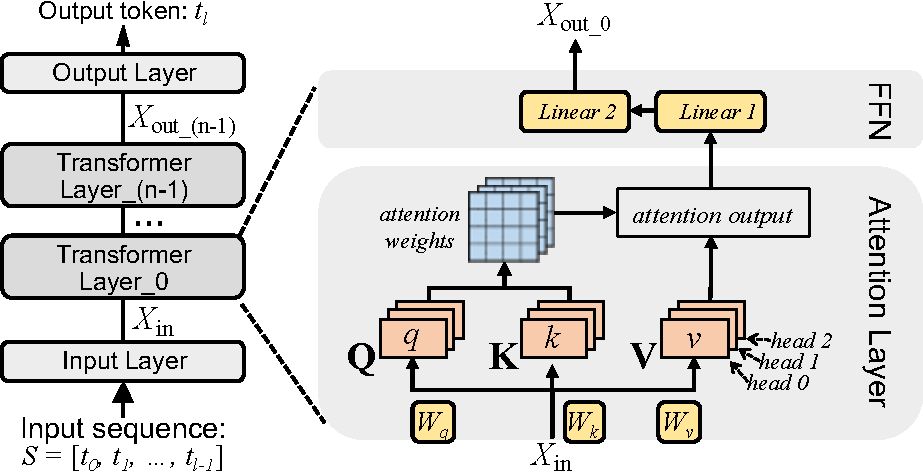
\includegraphics[width=3.4in, height=1.6in]{transformer.pdf}
	\vspace{-0.05in}
	\caption{The LLM model structure.}
	\label{fig:llm}
	\vspace{-0.1in}
\end{figure}

\subsection{Architecture and Workflow of Large Language Models}
\label{sec:llm-basic}


%A generative LLM typically consists of an input layer, tens of consecutive transformer layers, and an output layer, as shown in Figure~\ref{fig:llm}. Assume an input sequence with \( l \) tokens denoted as \( S = [t_0, t_1, \dots, t_{l-1}] \) and an LLM with \( n \) transformer layers. This sequence is first transformed into a tensor \( X_{\text{in}} \) with shape \( l \times d \) by the input layer, where \( d \) is the model’s hidden dimension. \( X_{\text{in}} \) then passes through the first transformer layer, resulting in an intermediate output tensor \( X_{\text{out\_0}} \) that maintains the shape \( l \times d \). This \( X_{\text{out\_0}} \) becomes the input for the subsequent transformer layer. The final block's output, \( X_{\text{out\_(n-1)}} \), is passed to the output layer, generating the first new token \( t_l \). 
%Then, the newly generated token is fed back into the input layer to generate the next token. This process repeats until either the maximum token limit is reached or a special end-of-sequence (EOS) token is generated, signaling the end of the LLM inference process. The generation of each token is referred to as an \textit{iteration}. The process of generating the first token is called the \textit{prefill} phase, while the subsequent token generation is known as the \textit{decoding} phase.

\noindent \textbf{Model inference.}
\cp{A generative large language model (LLM) consists of an input layer, a stack of transformer layers, and an output layer, as illustrated in Figure~\ref{fig:llm}. Given an input sequence \( S = [t_0, t_1, \dots, t_{l-1}] \) of \( l \) tokens, the input layer maps it to a tensor \( X_{\text{in}} \in \mathbb{R}^{l \times d} \), where \( d \) is the hidden dimension. This tensor is then processed sequentially through \( n \) transformer layers. Each layer must complete its computation before passing its output \( X_{\text{out}_i} \in \mathbb{R}^{l \times d} \) to the next layer, forming a strictly layer-by-layer dependency. The final layer output \( X_{\text{out}_{n-1}} \) is then fed into the output layer to generate the next token \( t_l \). The new token is appended to the input sequence and reprocessed to generate subsequent tokens.This iterative process continues until reaching the maximum token limit or a special end-of-sequence (EOS) token. The generation of the first token is referred to as the \textit{prefill} phase, while the generation of subsequent tokens is termed the \textit{decoding} phase.}


%\textbf{KV Cache Used in Decoding Phase. }
%Since each iteration’s input sequence shares many tokens with the previous iteration, some identical intermediate data (i.e., key and value tensors) are redundantly recalculated, leading to wasted computational resources across iterations.
%To reduce computational overhead, the key and value tensors generated by each transformer layer during an iteration are stored (referred to as the \textit{KV cache}) for reuse in the subsequent iteration. Specifically, in the 0th iteration, the keys and values of all tokens in the input sequence \( S \) must be generated. In subsequent iterations, only the single newly generated token from the last iteration is passed into the LLM, so only that token’s KV needs to be calculated. Due to this difference in computation patterns, researchers often refer to the 0th iteration as the \textit{prefill} phase, with all subsequent iterations collectively known as the \textit{decoding} phase.


%Each transformer layer consists of an attention layer and a feed-forward network (FFN) (we omit the description of layer normalization and residual connections for simplicity in Figure~\ref{fig:llm}). 
%During the prefill phase, the input tensor \( X_{\text{in}} \) is passed through three weight matrices, \( W_q \), \( W_k \), and \( W_v \), to generate three 3D transient tensors: query (Q), key (K), and value (V). Each of these tensors consists of multiple heads (e.g., 3 in Figure~\ref{fig:llm}), with each head containing a 2D tensor referred to as \( q \), \( k \), or \( v \). 
%The Q and K tensors are then used to produce attention weights, where each head has one corresponding 2D attention weight matrix. 
%Each value in the attention weights indicates the relevance of one token to another. 
%The attention weights are then multiplied by the V tensor to form the attention output. 
%This output is passed through a feedforward network (FFN), which consists of two linear layers, ultimately producing the output tensor \( X_{\text{out}} \), with the same shape as \( X_{\text{in}} \).
\noindent \textbf{Transformer layer computation.}
\cp{Each transformer layer mainly consists of an attention layer and a feed-forward network (FFN), as shown in Figure~\ref{fig:llm}. During the prefill phase, the input tensor \( X_{\text{in}} \) is projected by the weight matrices \( W_q \), \( W_k \), and \( W_v \) to produce the query (\( Q \)), key (\( K \)), and value (\( V \)) tensors. Each tensor consists of multiple attention heads (e.g., three in Figure~\ref{fig:llm}), where each head corresponds to a 2D tensor denoted as \( q \), \( k \), and \( v \), respectively.
The attention weights, computed from \( Q \) and \( K \), represent token relevance and are applied to \( V \) to obtain the attention output. This output then passes through a two-layer FFN to produce \( X_{\text{out}} \), which has the same shape as \( X_{\text{in}} \).}



\begin{figure}
	\centering
	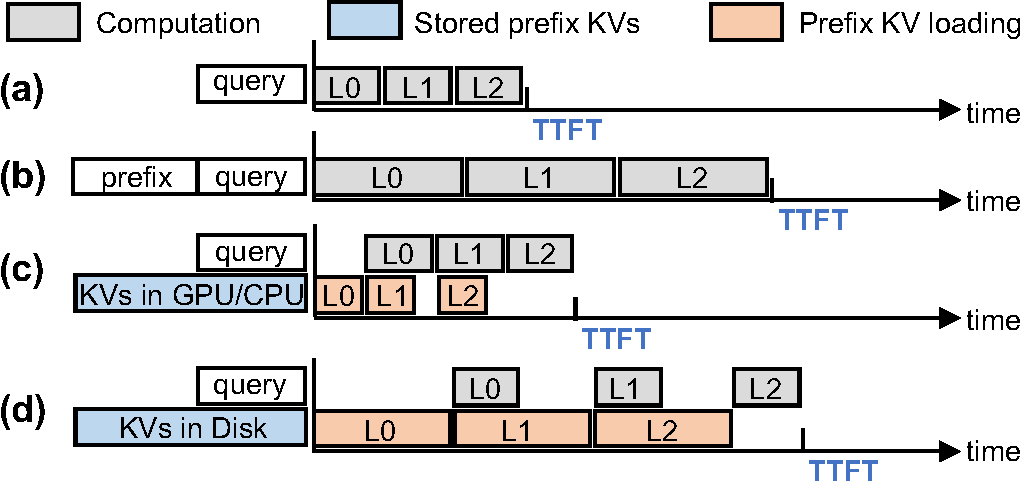
\includegraphics[width=3.4in, height=1.6in]{pkvloading.pdf}
	\caption{The TTFTs of various cases. Assume the LLM model consists of three transformer layers, denoted as `Lx'.}
	\label{fig:pkvloading}
\end{figure}

\subsection{Shared Prefixes and Storage System}
\label{sec:iobottleneck}
\noindent \textbf{Long TTFT due to the use of context-rich prefixes.}
\cp{Directly using large models for inference may yield suboptimal results. Specifically, when asked about recent events absent from the training data, the model can produce incorrect or misleading responses due to issues~\cite{siren-arxiv23}. To enhance response quality, applications often augment user \textit{queries} with context-rich \textit{prefixes}, forming complete \textit{requests} that are fed into the LLM as input sequences.
For example, Retrieval-Augmented Generation (RAG)~\cite{rag-nips20} retrieves external documents relevant to the user query. Advanced GPT plugins, such as Chameleon~\cite{chameleon-nips23}, embed tool definitions in the system prompt and use few-shot examples to guide complex reasoning. Multi-turn dialogue systems~\cite{attentionstore-atc24} incorporate previous question–answer pairs to better capture user intent, while self-consistency~\cite{selfcons-ase23} improves accuracy by generating multiple responses and aggregating them through voting.}
%Directly using large models for inference can lead to suboptimal results. For instance, when queried about a recent event not included in the model's training data, the model might provide incorrect answers. Additionally, due to issues such as hallucinations, the model's responses might contain inaccurate or misleading information~\cite{siren-arxiv23}. To improve response quality, applications often prepend user \textit{queries} with additional context-rich \textit{prefixes} to form complete \textit{requests}, which are then fed into the LLM as input sequences.
%For example, Retrieval-Augmented Generation (RAG)~\cite{rag-nips20} searches external knowledge bases for documents relevant to the user's query. Advanced GPT plugins, such as Chameleon~\cite{chameleon-nips23}, include tool definitions in the system prompt and use few-shot examples to guide the LLM in performing complex reasoning tasks. Multi-turn dialogue applications~\cite{attentionstore-atc24} add previous question-answer pairs to the user's latest query for better intent understanding, while the self-consistency technique~\cite{selfcons-ase23} generates multiple responses to the same query and uses voting to improve accuracy.

\cp{Figures \ref{fig:pkvloading}(a) and \ref{fig:pkvloading}(b) show that although context-rich prefixes enhance response quality, they substantially increase the delay before the first token is produced, known as the time to first token (TTFT). For example, Chameleon adds more than 2,600 tokens before each user query \cite{chameleon-prompt}. Given that an average real-world query contains approximately 750 tokens \cite{sharegpt}, this quadruples the input length and increases TTFT by up to nine times for the OPT-30B model. Such latency severely affects user experience in TTFT-sensitive applications such as real-time chatbots and also reduces system throughput, leading to higher operational costs.}


%Figure~\ref{fig:pkvloading}(a) and Figure~\ref{fig:pkvloading}(b) show that while these context-rich prefixes improve the quality of responses, they also significantly increase the time-to-first-token (TTFT), which is the delay before the model generates the first token. For instance, the Chameleon system adds over 2,600 tokens of context before the user's query~\cite{chameleon-prompt}. Given that the average real-world user query is about 750 tokens~\cite{sharegpt}, this increases the request token count by more than 4$\times$, extending the TTFT by 9$\times$ for the OPT-30B model due to the additional computation. This can negatively impact user experience, especially in TTFT-sensitive applications like real-time chatbots. 
%Besides, it also degrades the system's overall throughput and increases the enterprise costs.	
%This paper focuses on reducing TTFT during the prefill phase without altering the decoding phase. Note that shortening TTFT also reduces decoding latency for other requests, as modern systems use continuous batching, where the decoding of existing and newly-arrived requests are processed together after the completion of the prefill of the new requests~\cite{orca-osdi22}.

\noindent \textbf{Prefix KV storage systems and I/O bottleneck.}
Researchers have observed that these prefixes are often partially or completely shared across different requests~\cite{sglang-arxiv23, chunkattention-arxiv24, cachegen-sigcomm24, ragcache-arxiv24, promptcache-mlsys24, attentionstore-atc24}. For example, similar queries might retrieve partially or entirely the same related documents using RAG; the same GPT plugin can be used multiple times, resulting in identical system prompts across requests. 
Recomputing the K and V tensors in Figure~\ref{fig:llm} for the same prefix leads to wasted computational resources and increased TTFT. To optimize TTFT, existing systems store and reuse the K and V tensors of these shared prefixes (referred to as \textit{prefix KV cache} or simply \textit{prefix KV}). Note that the Q tensor of the prefix is not stored, as it is not needed for subsequent computations~\cite{attentionstore-atc24}. When a new request with a repeated prefix arrives, the system asynchronously preloads its prefix KVs into GPU memory, thereby reducing TTFT during the prefill phase of the new request.


\begin{figure}
	\centering
	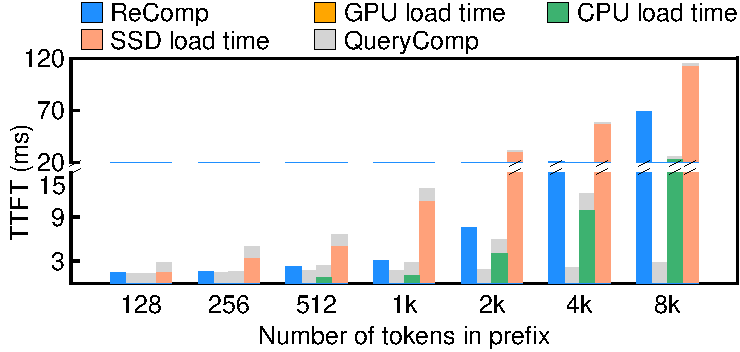
\includegraphics[width=3.3in, height=1.55in]{pload_bottleneck.pdf}
	\vspace{-0.1in}
	\caption{TTFT breakdown.
				`ReComp' refers to not reusing the prefix KV. `QueryComp' denotes the remaining computation after loading the prefix KV. }
%	\vspace{-0.1in}
	\label{fig:pload-bottleneck}
	\vspace{-0.15in}
\end{figure}

\cp{\subsection{Limitations of Existing Prefix KV Storage Systems}}



\begin{table}[t]
	\centering
	\caption{\cp{Comparison of prefix KV storage designs.}}
	\label{tab:pkv_comparison}
	\setlength{\tabcolsep}{3pt}  
	\renewcommand{\arraystretch}{1.15}
		\begin{tabular}{lccccc}
			\specialrule{1.2pt}{0pt}{2pt}
			\textbf{System} & \makecell{\textbf{CPU}\\\textbf{Memory}} & \textbf{Disk} & \makecell{\textbf{Import.}\\\textbf{Aware}} & \textbf{Caching} & \textbf{Prefetching} \\
			\specialrule{1.2pt}{0pt}{2pt}
			\textit{PromptCache}~\cite{promptcache-mlsys24} & \cmark & \xmark & \xmark & \cmark & \cmark \\
			\textit{SGLang}~\cite{sglang-arxiv23}           & \cmark & \xmark & \xmark & \cmark & \cmark \\
			\textit{RAGCache}~\cite{ragcache-arxiv24}       & \cmark & \xmark & \xmark & \cmark & \cmark \\
			\textit{ChunkAttention}~\cite{chunkattention-arxiv24} & \cmark & \xmark & \xmark & \xmark & \cmark \\
			\textit{AttentionStore}~\cite{attentionstore-atc24}   & \cmark & \cmark & \xmark & \cmark & \cmark \\
			\textit{IMPRESS}~\cite{impress-fast25}          & \cmark & \cmark & \cmark & \cmark & \xmark \\
			\textit{\pname{} (Ours)}          & \cmark & \cmark & \cmark & \cmark & \cmark \\
			\specialrule{1.2pt}{0pt}{2pt}
		\end{tabular}
\end{table}


\cp{An effective prefix KV storage system must satisfy two key requirements. First, it must provide sufficient storage capacity to hold a large number of prefix KVs. Second, it must ensure low latency for prefetching prefix KVs, as excessive loading delay can become a bottleneck in LLM inference and limit the reduction of time-to-first-token (TTFT).
To achieve these goals, techniques such as caching, prefetching, and importance-aware loading  
are often employed to reduce I/O overhead and improve end-to-end efficiency. 
However, as summarized in Table~\ref{tab:pkv_comparison}, 
existing systems optimize only a subset of these dimensions, 
and none achieves a comprehensive solution across all aspects.}

\cp{\paragraph{GPU/CPU-Memory-Only Storage}  
Systems such as PromptCache~\cite{promptcache-mlsys24}, 
SGLang~\cite{sglang-arxiv23}, 
RAGCache~\cite{ragcache-arxiv24}, 
and ChunkAttention~\cite{chunkattention-arxiv24} 
store prefix KVs solely in GPU and/or CPU memory to minimize prefetch latency, 
as illustrated in Figure~\ref{fig:pkvloading}(c). 
This design achieves low TTFT by avoiding I/O operations and typically employs caching and prefetching 
to further reduce latency. 
However, GPU and CPU memory are inherently capacity-limited, 
causing these systems to quickly exhaust available storage under long-context or multi-session workloads. 
\zrdnew{For example, even with two A100 nodes (each equipped with 40 GB of GPU memory) and a total of 120 GB of CPU memory, a large model such as Llama-2-70B-Chat can only store around 300 K tokens of KV caches—roughly equivalent to the chat histories of 15–20 users. In more demanding multi-agent applications, where several agents continuously exchange information within a single session, the accumulated context can easily expand to millions of tokens, leading to a KV cache size of over 1 TB.}
As a result, while they excel in latency reduction, they fail to scale to large-context scenarios.}

\cp{\paragraph{Hybrid CPU-and-Disk Storage}  
To overcome the capacity constraint, 
AttentionStore~\cite{attentionstore-atc24} stores prefix KVs across both CPU memory and disk, 
providing sufficient capacity for large-context inference. 
Nevertheless, this design introduces new latency bottlenecks: 
disk-to-GPU data transfer cannot always be overlapped with computation, 
especially under heavy or preemptive workloads. 
As shown in Figure~\ref{fig:pkvloading}(d) and Figure~\ref{fig:pload-bottleneck},
loading prefix KVs from SSD significantly increases TTFT,
as the I/O latency, which accounts for 51\% to 98\% of the total, rarely overlaps with query computation.
Therefore, while hybrid storage improves capacity, 
it does so at the cost of prefetch efficiency, failing to balance both latency and scalability.}


\cp{\paragraph{Importance-Aware KV Loading}  
To mitigate the I/O bottleneck caused by loading prefix KVs from storage, IMPRESS~\cite{impress-fast25} introduces a novel approach that loads only the most important KVs to reduce I/O latency while maintaining comparable model accuracy. However, these selected KVs still lie on the critical path of model inference.
Although prior works employ prefetching to overlap data loading with model computation and thereby reduce I/O latency, this strategy fails in IMPRESS. The selection and loading of important KVs for the next layer depend on the computation results of the current layer, making it impossible to determine which KVs to prefetch in advance. Consequently, the I/O latency of these KVs remains exposed on the critical path, limiting end-to-end inference efficiency.}










%An effective prefix KV storage system must meet two requirements. First, it needs sufficient storage capacity to hold enough prefix KVs. Second, the latency for prefetching the prefix KV must be low. Otherwise, it will become a bottleneck of the LLM inference, limiting the reduction of TTFT. 
%Currently, no system can simultaneously meet these two requirements across various scenarios.
%Most existing systems store prefix KVs only in GPU and/or CPU
%memory~\cite{promptcache-mlsys24, sglang-arxiv23, ragcache-arxiv24,
%chunkattention-arxiv24}, as shown in Figure~\ref{fig:pkvloading}(c), to reduce
%TTFT. However, the limited space in GPU and CPU memory quickly becomes
%exhausted. Although the latest prefix KV storage system,
%AttentionStore~\cite{attentionstore-atc24}, stores the prefix KV on both CPU
%memory and disk to provide sufficient storage space, it doesn’t fundamentally
%reduce the load time, as the latency from disk cannot be fully hidden by
%computation in some cases as shown in Figure~\ref{fig:pkvloading}(d).  
%Thus, this approach may fail under heavy request loads or in preemptive scheduling scenarios, due to the bottleneck of disk I/O.
%\zrdnew{IMPRESS~\cite{impress-fast25} proposes that loading only important KVs to reduce I/O latency while maintaining comparable accuracy. However, the identification and loading of important KVs for the next layer depend on the computation results of the current layer, which makes it impossible to prefetch them during the current layer's computation. As xxx shows, although this approach reduces the I/O volume, it fails to leverage the opportunity to parallelize I/O with computation, resulting in the I/O bandwidth being underutilized during computation.}
%Figure~\ref{fig:pload-bottleneck} shows the TTFT breakdown for recalculating
%shared prefixes versus loading and reusing prefix KVs from different storage
%media (i.e., GPU memory, CPU memory, and SSD). We vary the number of input prefix tokens from
%128 to 8k. The ``load''  time represents the I/O latency that cannot be hidden by
%query computation. 
%It shows that loading prefix KVs from GPU or CPU results in shorter TTFT compared to recomputation, but loading from SSD leads to longer TTFT. This is due to the I/O latency from SSD to GPU, which is rarely hidden by query computation and accounts for 51\%-98\% of the total TTFT.
%Consequently, prefix KV loading has become a new bottleneck in model inference, particularly for longer prefixes.



\subsection{Not All KVs Are Equally Important}
Recent research~\cite{h2o-nips23, infinigen-osdi24, flexgen-icml23, scissorhands-nips23} indicates that not all tokens' KVs are equally important for maintaining LLM inference accuracy. These methods generate and store the full set of KVs during the prefill phase, then  identify and discard the less important tokens' KVs during decoding by analyzing the attention weights. This approach reduces the computational load during the decoding phase while maintaining comparable LLM inference accuracy.

Inspired by this, we propose an importance-informed three-tiered prefix KV
\zrd{caching and speculative prefetching system} that encompasses GPU memory, CPU memory, and disk storage. \zrd{Our system addresses the disk I/O bottleneck through a two-pronged approach: selective loading and speculative prefetching. When reusing prefix KVs, we selectively load only important KVs for prefill and decoding computations, while unimportant tokens' KVs are discarded. To further optimize I/O efficiency, we propose a \technew{} mechanism that uses the current layer's important token indices to predict and prefetch the next layer's important KVs during computation, effectively overlapping I/O operations with computation. This integrated approach of selective loading combined with cross-layer speculative prefetching fundamentally alleviates the disk bottleneck by both reducing the total I/O volume and moving critical I/O operations off the inference critical path, thereby significantly reducing TTFT.} 
%When
%reusing prefix KVs, we aim to load only important KVs
%%  rather than fetching them
%% all. 
%% \wj{Only important prefix tokens' KVs participate in prefill and decoding
	%% computations, while unimportant tokens' KVs are discarded.}
%for prefill and decoding computations, while unimportant tokens' KVs are discarded.
%Selectively loading the important KVs can
%fundamentally alleviate the disk
%bottleneck, thereby reducing TTFT.

% when reusing prefix KVs 


\cp{\section{Design Challenges of \pname{}}}
\label{motiv}

\begin{figure}
	\centering
	\subfigure[Recall Ratio]{
		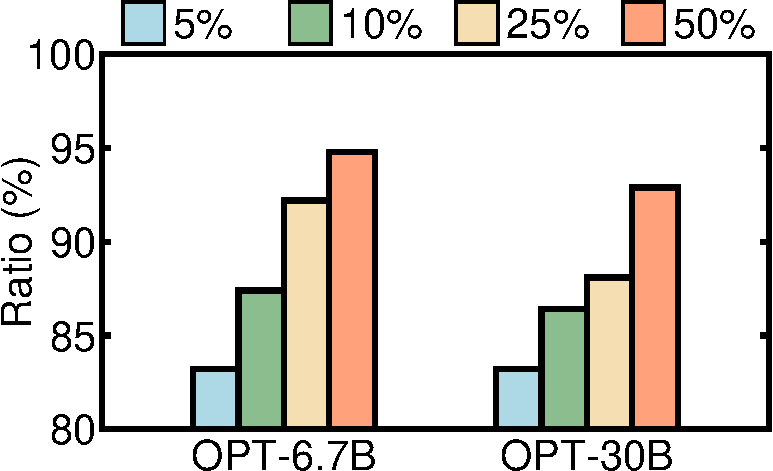
\includegraphics[width=1.5in, height=1in]{static_recall.pdf}
		\label{fig:static-recall}
	}
	\hspace{0.06in}
	\subfigure[Generation Quality]{
		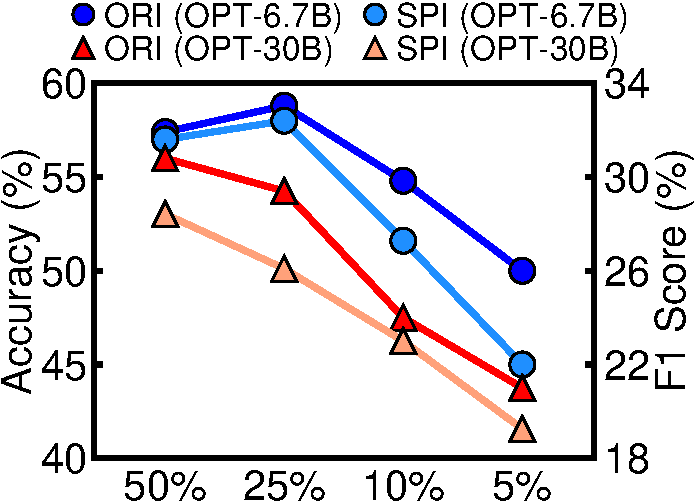
\includegraphics[width=1.5in, height=1in]{static_acc.pdf}
		\label{fig:static-acc}
	}
	\caption{The recall ratios and the impacts on model generation quality of the static pre-identification method (SPI) under various important token retention percentages. `ORI' denotes the baseline where the SPI method is not applied.}
	\label{fig:static_methods}
\end{figure}


\noindent \textbf{Challenge 1: Importance identification introduces high I/O overhead for prefix KV loading.}
\cp{Existing methods identify important KVs by loading all prefix keys (K) into GPU memory~\cite{h2o-nips23, infinigen-osdi24, flexgen-icml23, scissorhands-nips23}, 
so reducing only the loading time of values (V) yields limited TTFT gains. 
A static alternative records important tokens for each prefix and loads only their KVs when reused, 
reducing I/O but ignoring that token importance is query-dependent. 
In RAG, for example, different queries sharing the same document prefix may attend to different segments, 
causing static selection to miss critical tokens and degrade accuracy. 
We evaluate this limitation using OPT-6.7B on RTE~\cite{lmeval} and OPT-30B on SQuAD~\cite{squad-arxiv18}, 
measuring accuracy and F1 score~\cite{cachegen-sigcomm24}, respectively. 
As shown in Figure~\ref{fig:static_methods}, even with recall ratios above 80\%, 
missing key KVs reduces accuracy by up to 5\% on RTE and 3.3\% on SQuAD. 
These results motivate a dynamic approach that identifies important tokens per query while minimizing I/O overhead.}





%Existing methods must load all prefix keys into GPU
%memory to compute attention weights and then identify important
%KVs~\cite{h2o-nips23, infinigen-osdi24, flexgen-icml23,
%	scissorhands-nips23}. 
%Reducing only the loading time of prefix values limits TTFT reduction.
%
%A straightforward approach to avoid loading all prefix keys is to statically record the identified important tokens for queries. Then, when another query with the same prefix arrives, only the KVs of pre-identified important tokens would be loaded, reducing the I/O time.
%However, this approach has a significant flaw. We observed that the importance
%of tokens within the same prefix can vary depending on the specific query. We
%intuitively explain the observation here. For example, in a RAG scenario,
%different queries might use the same document as the prefix, but the relevant
%answers could be found in different text segments of the prefix. 
%Thus, the method that pre-identifies important tokens could miss critical ones, substantially degrading the accuracy of LLM inference.

% To validate this flaw, we test the important token recall ratio and its impact on model generation quality using two models and two datasets: OPT-6.7B on the RTE~\cite{lmeval} dataset and OPT-30B on the SQuAD~\cite{squad-arxiv18} dataset. We measure model generation quality using accuracy and F1 score, on these two datasets respectively. Figure~\ref{fig:static_methods} shows that although the recall rate exceeds 80\%, missing important KVs led to a drop in accuracy and F1 score of up to 5\% on the RTE dataset and 3.3\% on the SQuAD dataset.
% Hence, an intelligent method is required that can dynamically identify important tokens within a prefix for different queries while introducing minimal I/O overhead.




\begin{figure}
	\centering
	\subfigure[]{
		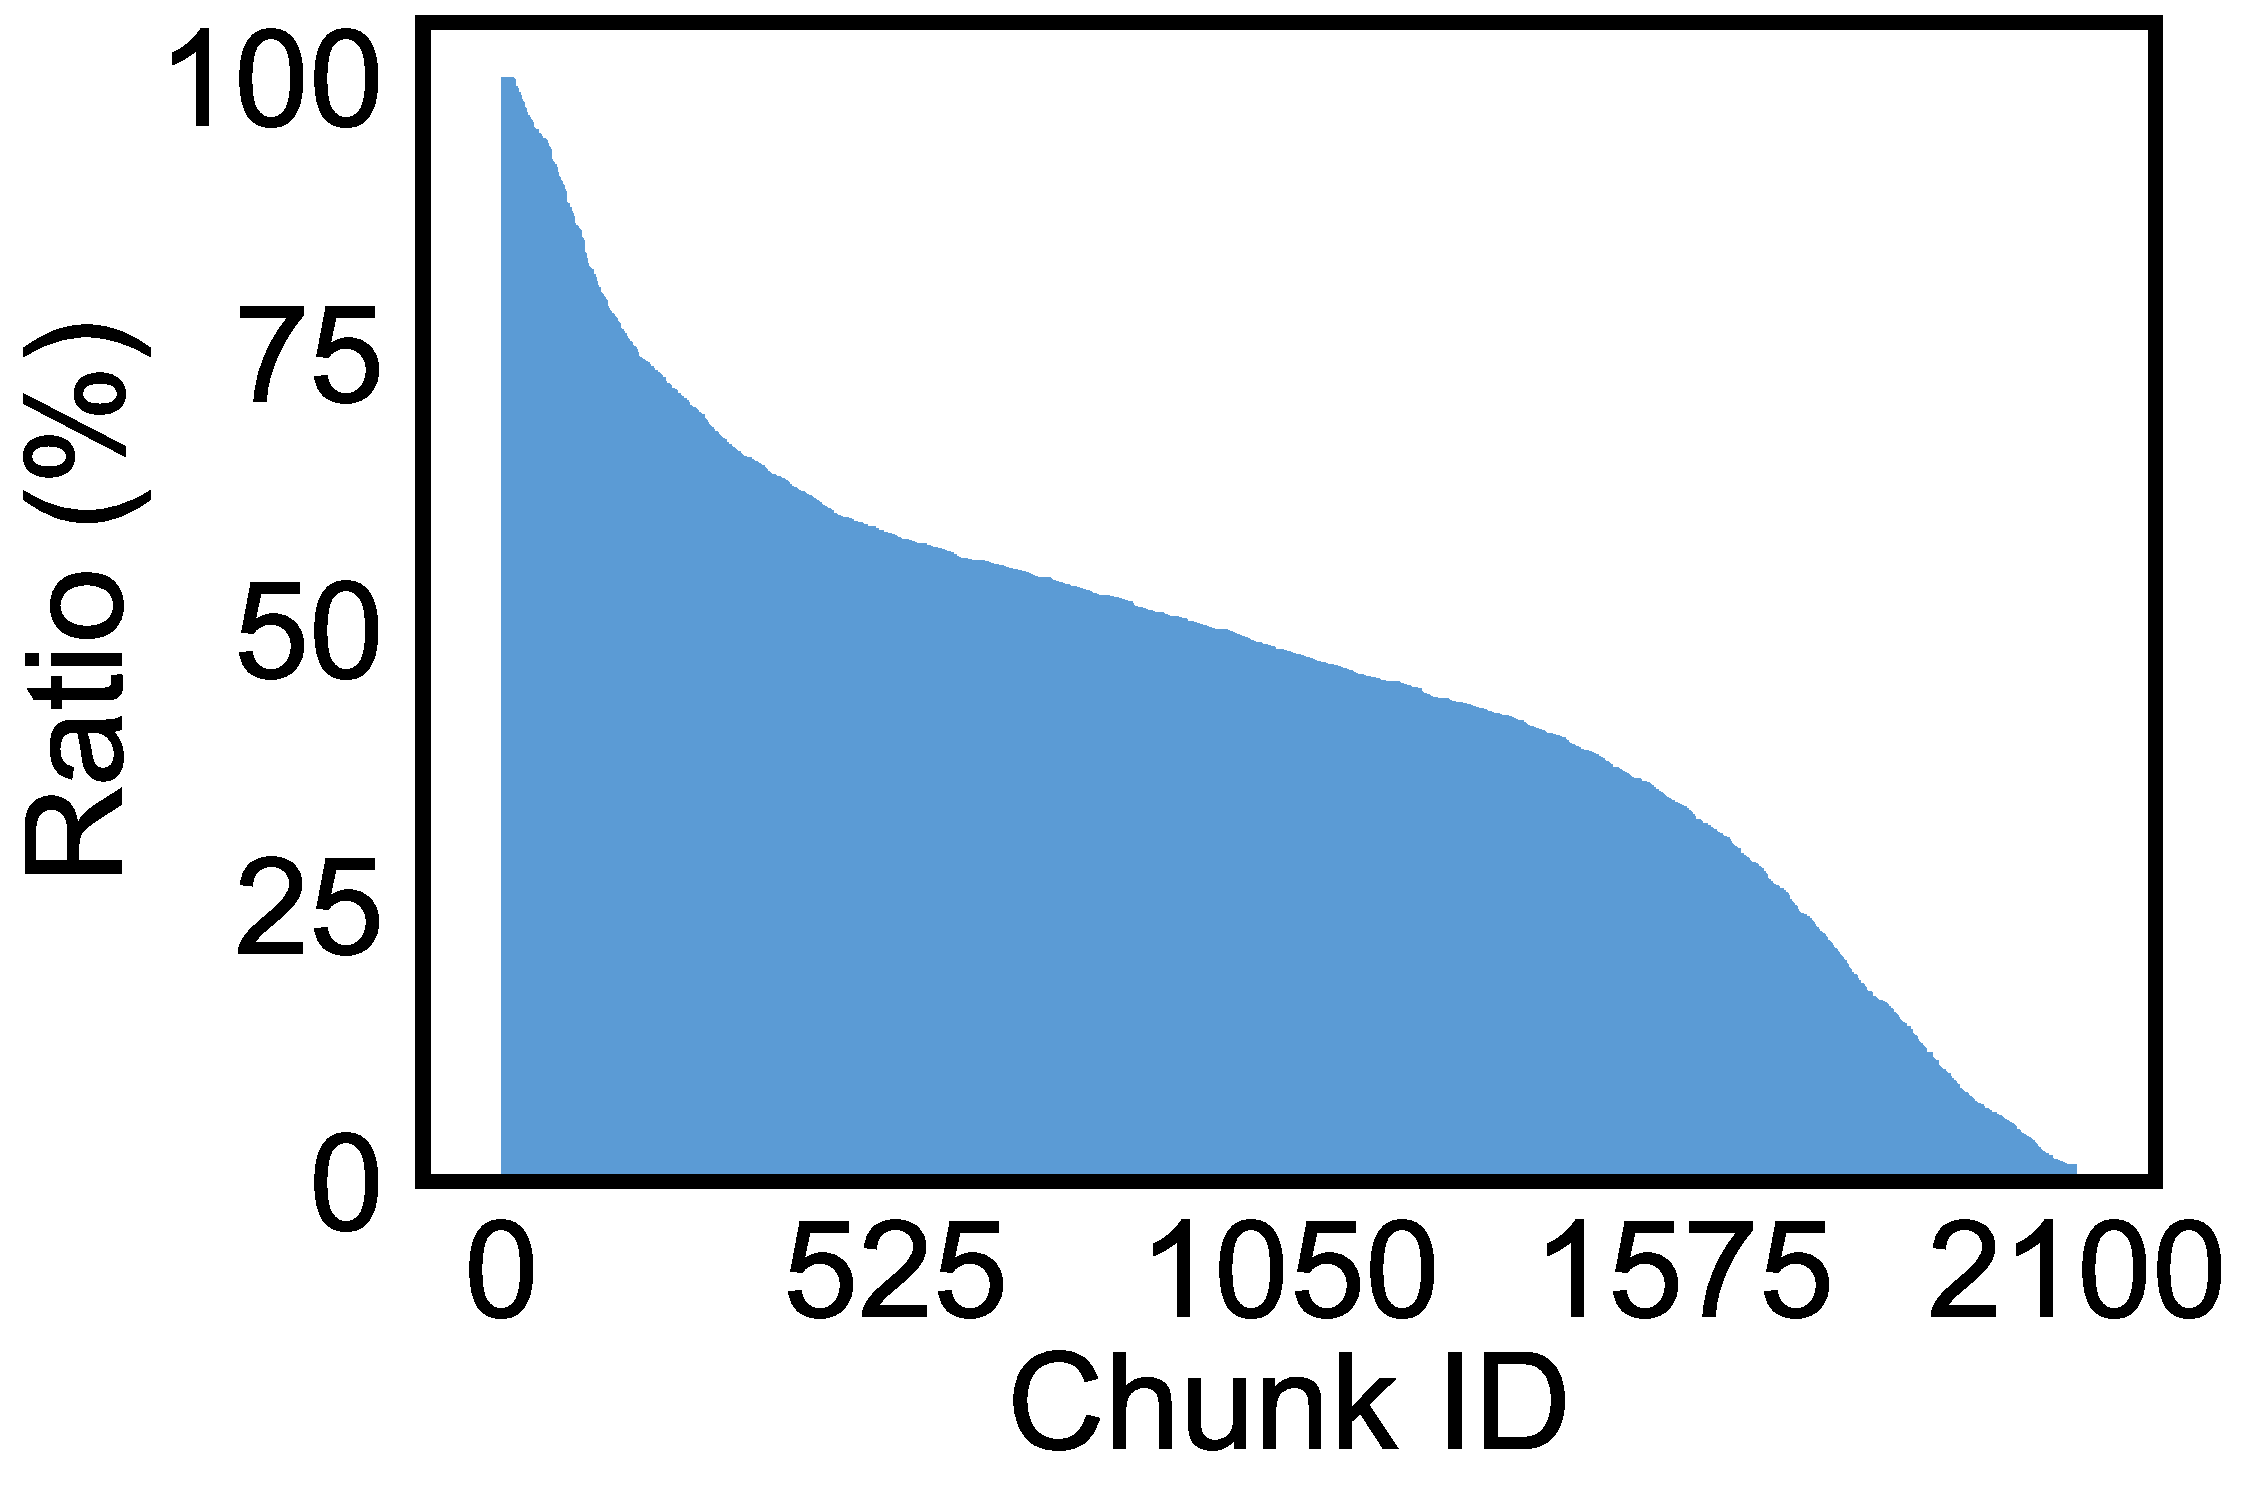
\includegraphics[width=1.5in, height=1in]{impratio_per_chunk.pdf}
		\label{fig:read_amplify}
	}
	\hspace{0.03in}
	\subfigure[]{
		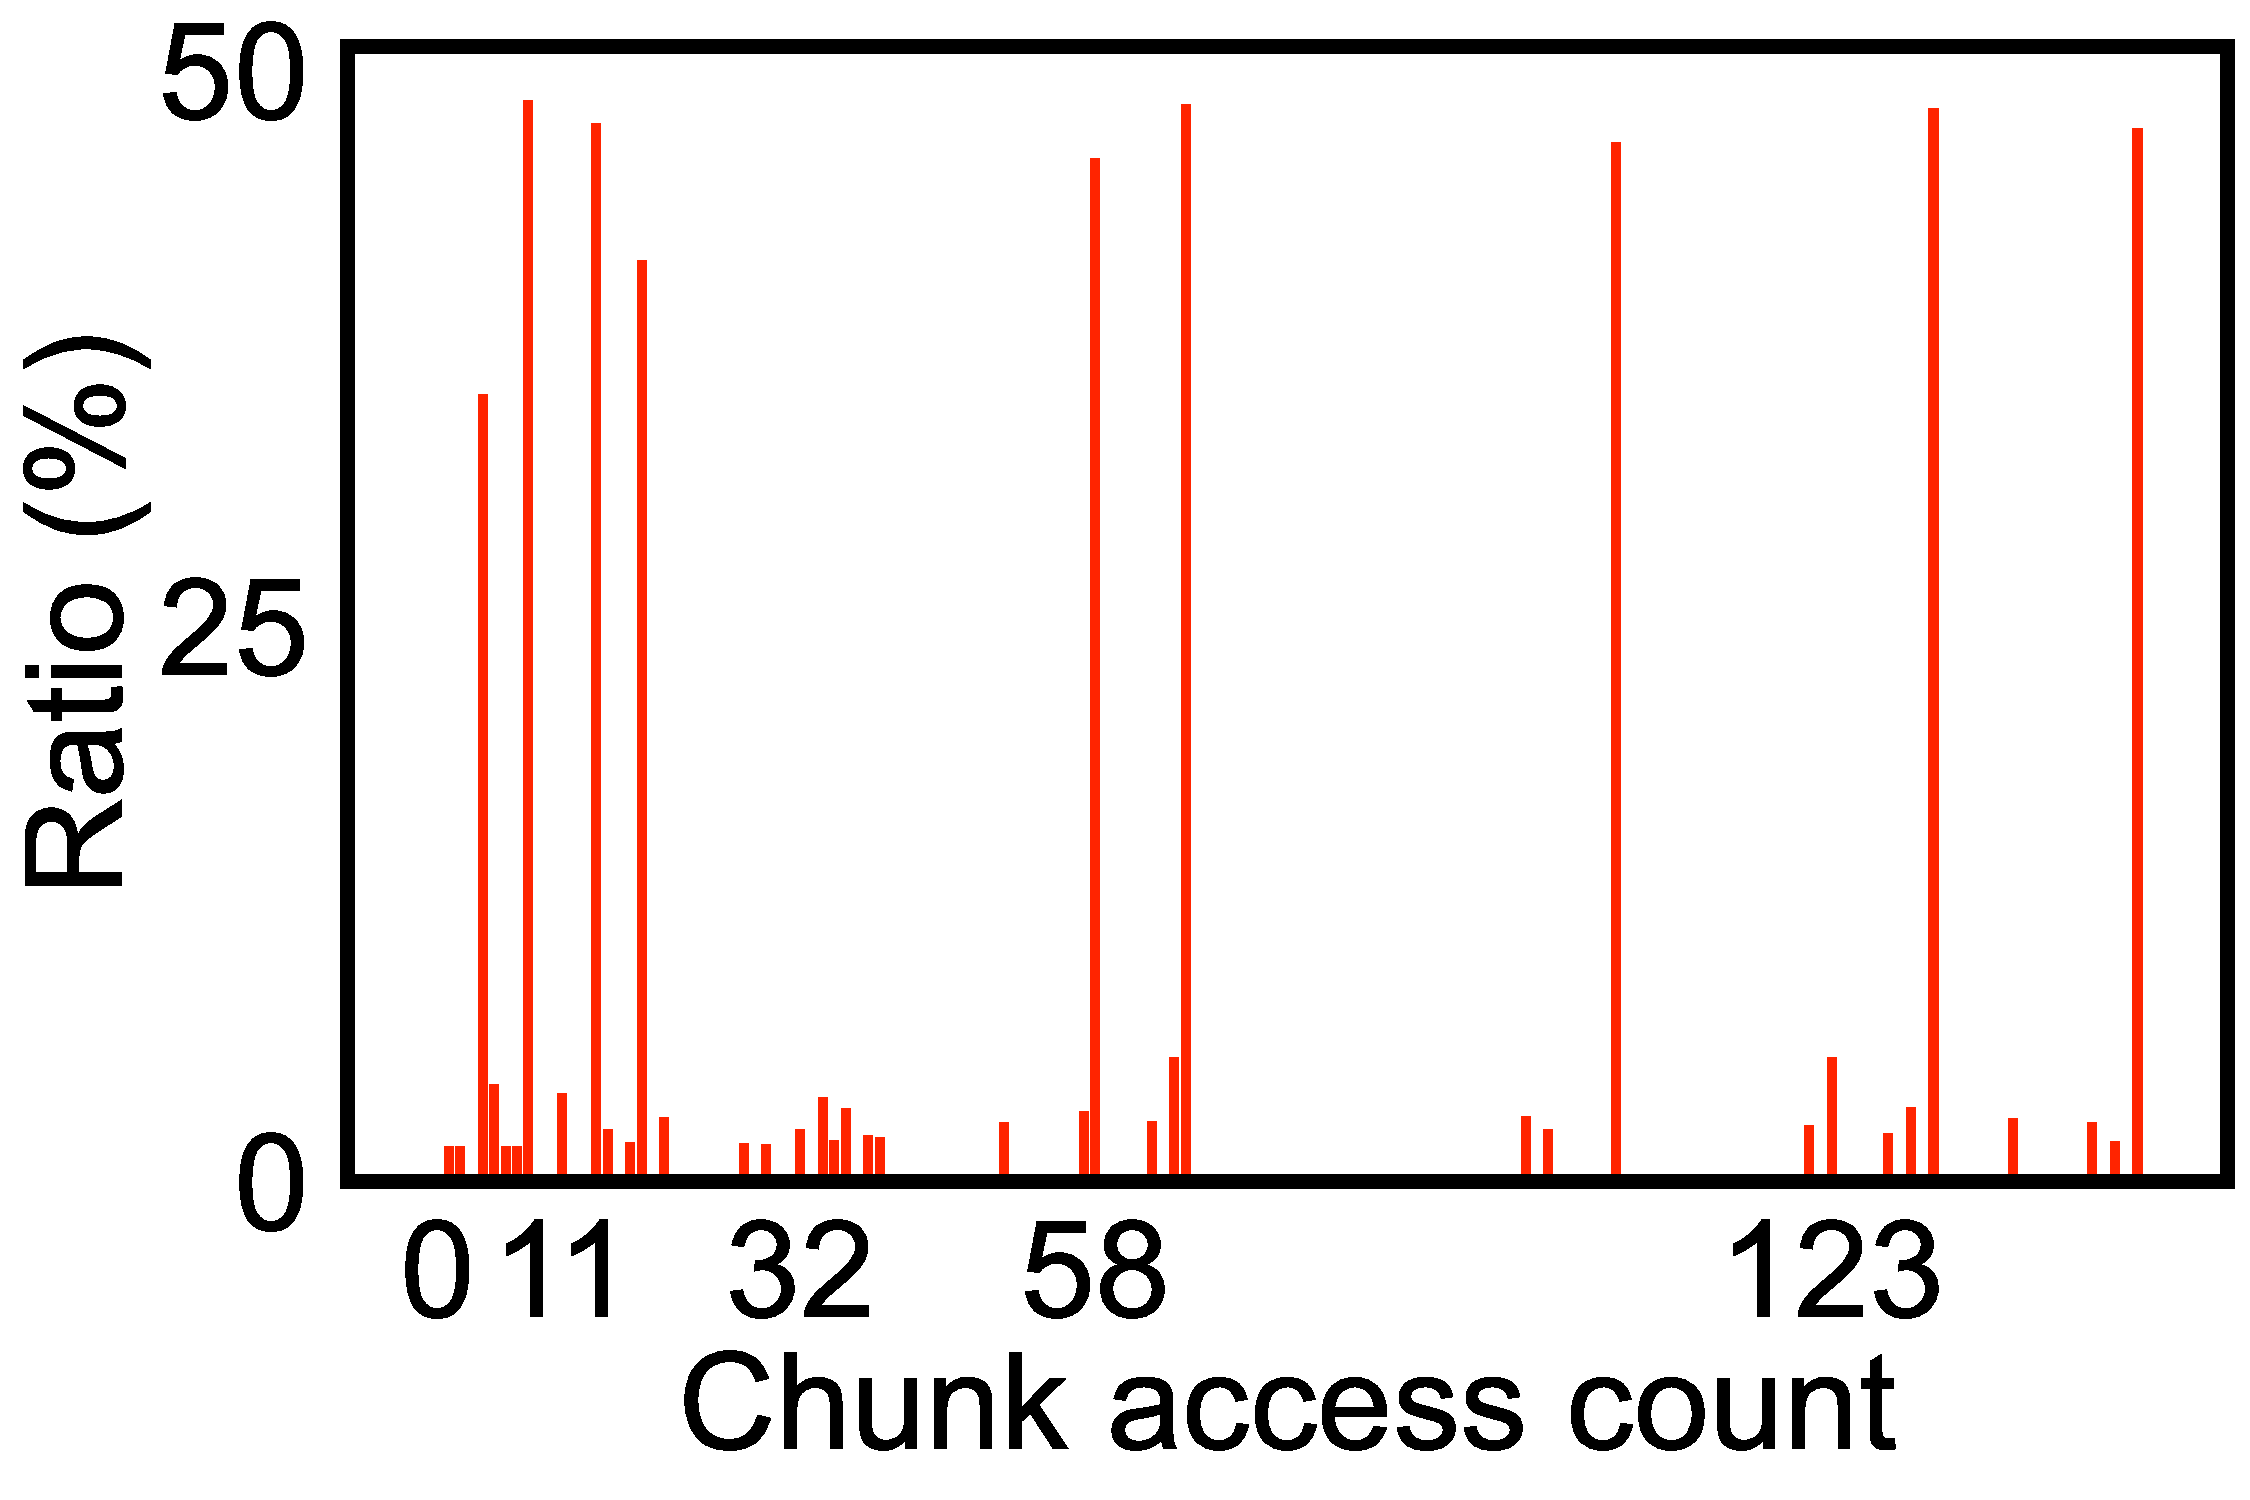
\includegraphics[width=1.5in, height=1in]{impratio_accesscount.pdf}
		\label{fig:imp_token_num}
	}
	\vspace{-0.2in}
	\caption{
		(a) The ratio of important KVs within each chunk. 
		(b) Average ratio of important tokens in all chunks for a given chunk access frequency.}
	\label{fig:cha2}
	\vspace{-0.2in}
\end{figure}

\noindent 
\zrdnew{
\textbf{Challenge 2: The distribution of important tokens is unknown before prefetching.}
Existing methods determine the important KVs of each layer by computing the attention weights of the current layer. As a result, the distribution of important tokens for the next layer is not available during the current layer’s computation. This prevents prefetching of the next layer’s important KVs while the current layer is being processed, leaving I/O bandwidth underutilized. }

\zrdnew{A straightforward alternative is to randomly prefetch KVs for the next layer without considering their importance, but this approach suffers from low accuracy and brings many unimportant tokens’ KVs into GPU memory, thereby wasting I/O bandwidth.}

\zrdnew{To verify this, we measured the recall rate of randomly prefetching KVs across two models and datasets, xxx and xxx. As shown in Figure xxx, when KVs were pre-fetched randomly, the recall rate was only xxx. This approach leads to a large number of unimportant KVs being loaded into CPU memory, which are not used during inference, resulting in wasted I/O bandwidth and GPU memory.}



\noindent 
%\textbf{Challenge 2: New approaches to store prefix KV and manage caches are required considering token's importance.}
\fvc{
\textbf{Challenge 3: The existing prefix KV storage and caching systems are suboptimal considering token's importance.}
}
Existing systems typically store and manage cache by grouping KV pairs from
several consecutive or all prefix tokens into
chunks~\cite{chunkattention-arxiv24, sglang-arxiv23, attentionstore-atc24,
hydragen-arxiv24}, which enhances the efficiency of disk reads and PCIe
transfers. 
% Each chuck contains multiple important and unimportant KVs. 
% When fetching important tokens' KVs, each request loads entire chunks into memory, including unimportant KVs. This leads to read 
% amplification and reduces effective read bandwidth. These unimportant KVs occupy additional cache space and decrease cache hit ratios.
% Moreover, directly managing chunks across both CPU and GPU cache spaces based on the traditional metrics like recency or frequency can degrade GPU cache hit ratios and increase the amount of data transferred over PCIe. 
% This is because they are oblivious of KV importance and do not consider the ratio of important KVs 
% in each chunk. Thus, they can place cold chunks with more important KVs in the CPU, while placing hot chunks with 
% fewer important KVs in the GPU. This misplacement reduces the hit ratio of important KVs in the GPU and requires 
% more important KVs to be transferred from the CPU to the GPU.
Each chunk contains a mix of important and unimportant KVs. When retrieving KVs for important tokens, entire chunks are loaded into memory, including the unimportant ones. This practice causes read amplification, diminishing effective bandwidth and filling cache with unnecessary data, which lowers cache hit ratios.

Furthermore, managing chunks in CPU and GPU caches based solely on traditional
metrics like recency or frequency can further reduce GPU cache hit ratios and
increase PCIe data transfers. This is because these metrics ignore the
importance of KVs and the proportion of important KVs in each chunk. As a
result, less critical chunks may occupy valuable GPU memory, while more critical
ones are relegated to the CPU memory. This misallocation decreases the GPU hit ratio
for important KVs and necessitates more data transfers between CPU and GPU memory.


We experimentally illustrate this challenge using OPT-6.7B on RTE. 
%We select the top 50\% most important KVs from each prefix for inference. 
% \wj{
We designate half of the prefix tokens as important and the remaining half as unimportant.
% }
Figure~\ref{fig:read_amplify} shows 
% the ratio of important KVs within each prefix KV chunk 
% that are selected for model inference. It shows 
that only 46\% of the KVs in the 
loaded chunks are important on average, leading to 2.2$\times$ read amplification. 
Figure~\ref{fig:imp_token_num} shows the ratio of important KVs for chunks with different access 
frequency. The hotness or coldness of a chunk is not related to the 
ratio of important KVs it contains. These observations 
% confirm the challenges mentioned above and 
underscore the need for new KV storage and cache management methods to reduce 
the loading of unimportant KVs from disk and improve cache hit ratios.

\section{\pname{} Design}
\label{design_mainpart}

\zrdnew{In this section, we present \pname{}, an importance-informed three-tier prefix KV \zrd{caching and prefetching }system. }
%We first introduce the system overview of SPEC and then elaborate on its three key components.}
First, we describe the overall architecture of \pname{} (\cref{sec:overview}). 
\zrdnew{Then, we introduce an I/O-efficient technique to identify important tokens (\cref{sec:techa}). 
Furthermore, we propose a prefetching technique to mitigate I/O bottlenecks by overlapping computation and I/O ({\cref{sec:technew}})}.
Finally, we explain how prefix KVs are managed across three storage tiers 
to further reduce the latency when loading them into GPU memory (\cref{sec:techb}).

\subsection{Overview}
\label{sec:overview}




We propose \pname{} to provide large storage capacity for prefix KVs while
ensuring efficient I/O accesses to reduce TTFT. The system is designed based on
three principles: (1) Using a minimal number of I/Os to identify the
important KVs within a prefix, allowing only the essential KVs to be loaded
during the prefill phase; 
\cp{(2) Since the I/Os for loading essential KVs lie on the critical path, we introduce data prefetching during model computation to mitigate the I/O overhead.}
(3) Since loading only important KVs could degrade
the efficiency of existing storage and caching systems, we optimize the
three-tier prefix KV management to improve cache hit
ratios and I/O efficiency.

\cp{Figure~\ref{fig:overview} illustrates the overall architecture of \pname{}, which consists of a data plane responsible for KV storage and a control plane that governs runtime data movement and computation scheduling.
In the data plane, all prefix key–value (KV) pairs are stored on disks in chunked form, while selected KVs are cached in either CPU or GPU memory. The two cache spaces are mutually exclusive to prevent redundancy. To mitigate I/O latency, essential KVs are prefetched during model computation to overlap data transfer with inference execution.}

\cp{The control plane manages GPU inference and includes three core modules: important token filtering (\cref{sec:techa}), data prefetching (\cref{sec:techc}), and prefix KV placement (\cref{sec:techb}). The token filtering module loads only a subset of key vectors to identify important tokens, reducing disk I/O. The prefetching module proactively loads critical KVs during computation to hide I/O overhead. The KV placement module manages KV distribution across disks, CPU memory, and GPU memory to maximize cache efficiency and eliminate redundancy.}

\begin{figure}
	\centering
	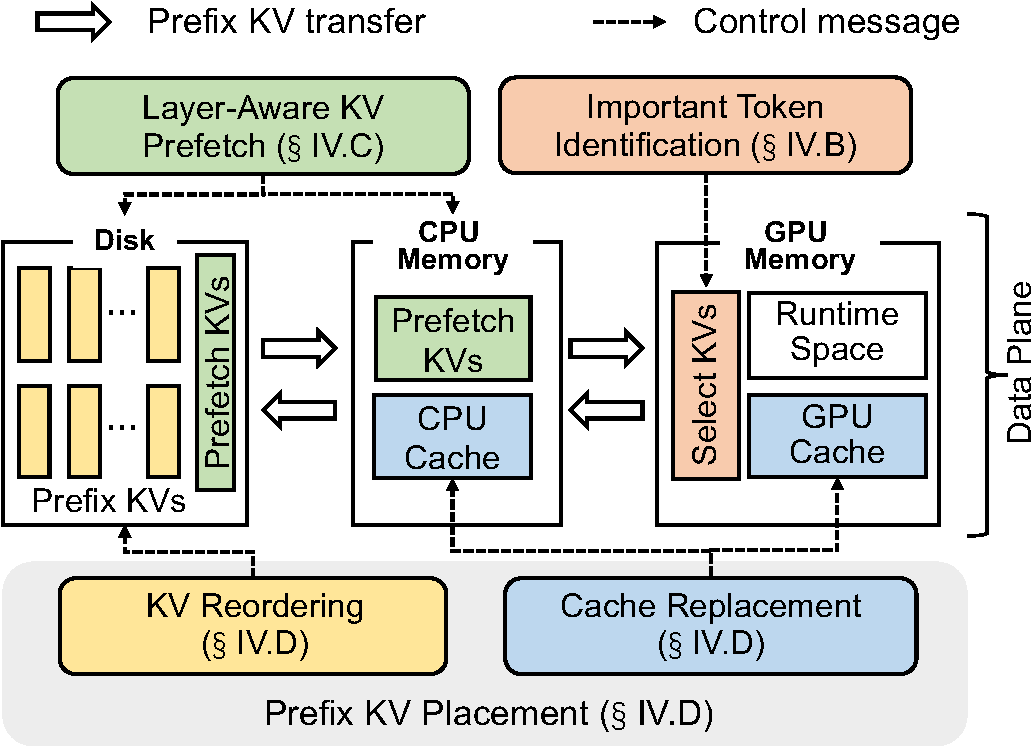
\includegraphics[width=3.3in]{overview.pdf}
	\caption{Overview of the \pname{} system.}
	\label{fig:overview}
	\vspace{-0.2in}
\end{figure}


\noindent \textbf{Dataflow of \pname{}.} 
Assume that a request $S=[t^p_0, t^p_1,...,t^p_{m-1}, t^q_0, t^q_1,...,t^q_{n-1}]$ arrives.
$m$ is the number of tokens in prefix and $n$ is the number of tokens in the query.
$t^p$ and $t^q$ denote the prefix and non-prefix tokens respectively. 
First, given the request, \pname{} searches the radix tree to find the longest common 
prefix subsequence from all previous requests~\cite{sglang-arxiv23, chunkattention-arxiv24}. 
Let's assume the result is  
%$R=[t^p_{i}, t^p_{i+1}, ..., t^p_j]$, whose KVs are 
$R=[t^p_0, t^p_1, ..., t^p_j]$, whose KVs are
stored in GPU memory, CPU memory, or disk.
There may also be some prefix tokens \( NR = [t^p_{j+1}, ..., t^p_{m-1}] \) that are not in the radix tree, and therefore their KVs do not exist in the system.
Next, \pname{} employs the I/O-efficient ITF method to identify 
the important tokens within $R$ , assuming $R_{important}=[t^p_{t}, t^p_{t+1}, ..., t^p_s]$ 
%($ i \leq t \leq s \leq j$) is identified. 
($ 0 \leq t \leq s \leq j$) is identified.
If KVs in $R_{important}$ are not in GPU memory, they are loaded from disk or CPU memory. 
The KVs of unimportant tokens in $R$ are not reused and do not participate in further inference.
Then, the loaded $R_{important}$, the tokens $NR$, and the tokens $[t^q_0, t^q_1,...,t^q_{n-1}]$   
are sent into LLM model, completing the remaining computations in the prefill phase.
Essentially, $R_{important}$ plus $NR$ becomes the defacto prefix used in the LLM inference,
replacing the set of \{$t^p$\} in $S$.
%Finally, the newly generated KVs for the prefix token in $R_{important}$ are stored on disk, 
%and the prefix tokens in $R_{important}$ are inserted into the radix tree for future reuse by other requests. 
Finally, the newly generated KVs for the prefix token in $NR$ are stored on disk, 
and the prefix tokens in $NR$ are inserted into the radix tree for future reuse by other requests. 
The decoding phase remains unchanged, following existing systems~\cite{alluneed-nips17}.

% \wj{
\noindent \textbf{Importance metric.} 
In this paper, we use the sum of values
in each column of the attention weight matrix as the token's importance,
following the same method in H2O~\cite{h2o-nips23}. A higher sum indicates greater
token importance. Our system is also compatible with other metrics for measuring
token importance~\cite{scissorhands-nips23, flexgen-icml23, infinigen-osdi24}.
% }

%\pname{} uses a radix-tree~\cite{sglang-arxiv23} 
%to manage the mapping from a token ID to its location.
%When a user request arrives, it searches the radix tree
%to identify its prefixes shared with previous requests. 
%For each token in the prefix, we design different
%dataflows depending on whether the token
%is an important token. 
%(1) If a token is an important token and exists
%in the radix-tree, its prefix KV will be moved
%to GPU if it does not exist in GPU.
%(2) If a token is an important token but does not
%exist in the radix-tree, its prefix KV will be
%generated through the prefill computation and decoding
%(illustrated in Section 2.1). After that, it is moved to GPU.
%(3) If a token is not an important token, \pname{}
%will substitue its KV with the KV of one important token 
%identified by ITF in the subsequent inference to
%reduce the amount of data for loading/generating 
%prefix KVs.

%\wj{
%When a user request arrives, it searches the radix tree 
%to identify its shared prefixes with previous requests. 
%For each token in the prefix, we design different 
%dataflows depending on whether the token is shared.
%(1) If a token is not shared, its prefix KV will be 
%generated through the prefill computation (illustrated in \cref{sec:llm-basic}). 
%Afterward, the token is inserted into the radix tree, 
%and its prefix KV is stored on disk for future reuse by other requests.
%(2) If a token is shared, it will be evaluated by the ITF 
%to determine if it is an important token. 
%If it is important and its prefix KV is not in GPU memory, 
%the prefix KV will be fetched to the GPU for subsequent inference computation. 
%If it is not important, its prefix KV will be not used for current request's computations.
%}


%(1) If the token ID does not exist in the radix-tree,
%indicating no shared prefix is found, \pname{} will
%insert the token into the radix-tree, perform a complete 
%prefill computation, split the computed prefix KVs into fixed chunks, 
%and stores them on disks. The stored prefix KVs are periodically 
%reordered and the relevant metadata are updated. 
%(2) If the token is found in the radix-tree,
%\pname{} will identify the location of important prefix KVs 
%in the multi-tier storage and move them to GPUs for
%further inference.
%(3) If a subset of tokens are found in radix-tree, indicating
%the current request has a partially shared prefix with
%previous requests, the system will first identify important
%KVs shared among the heads for the current query through ITF.
%Then, for the important KVs exist in the storage, they
%will be moved to GPU. For the remaining, they will be generated
%through prefill computation, along with all subsequent decoding phases 
%in GPUs. The prefix KVs including the newly generated KVs will be either 
%cached in GPU or CPU memory, or discarded (with a copy always retained on 
%disks). Their corresponding metadata are updated accordingly.


%\subsection{Insights of Important Tokens}
%\label{sec:insight}
% Empirical 
%\begin{figure}
%	\centering
%	\subfigure[Two Heads of K Tensors]{
%		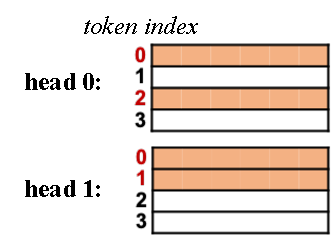
\includegraphics[width=1.5in, height=1in]{jcd-example.pdf}
%		\label{fig:jcd-example}
%	}
%	\hspace{0.06in}
%	\subfigure[Jaccard Scores Between Heads]{
%		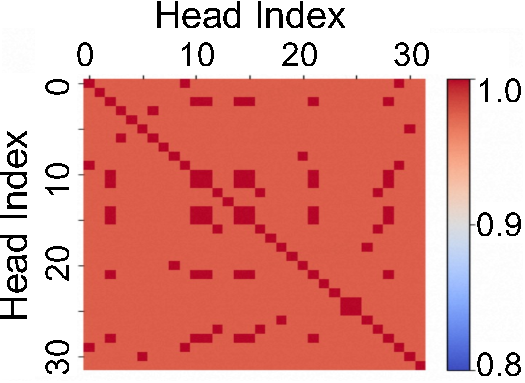
\includegraphics[width=1.5in, height=1in]{real-jcd-example.pdf}
%		\label{fig:real-jcd-example}
%	}
%	\vspace{-0.1in}
%	\caption{Examples of similarities. (a) The orange rows represent the important keys whose token indices are marked in red. (b) Darker squares indicate a higher similarity between the important token index sets of two heads.}
%	\vspace{-0.1in}
%\end{figure}
%
%
%
%%We highlight two key observations regarding the characteristics of important tokens.
%%Although we cannot strictly prove these observations mathematically for all LLMs and scenarios, we demonstrate the generality and practicality of these findings by showing the impact on accuracy when designs based on these observations are applied, across x datasets and x models.
%%, we will demonstrate the generality and practicality of these observations through accuracy evaluations after applying the corresponding techniques on x datasets and x models.
%
%%\vspace{-1.0ex}
%%\begin{framed}
%%\vspace{-1.4ex}
%%\noindent
%%\textbf{Observation I:}{
%%There is a high similarity in the set of important token indices 
%%across different heads within the same layer of an LLM.
%%}
%%\vspace{-1.4ex}
%%\end{framed}
%\noindent
%\textbf{Observation I:}{
%	There is a high similarity in the set of important token indices 
%	across different heads within the same layer of an LLM.
%}
%
%%\textbf{Observation 1.} \textit{There is a high similarity in the set of important token indices across different heads within the same layer.}
%
%As described in \cref{sec:llm-basic}, each token has K and V tensors for every head. We found that the set of important token indices is highly similar across different heads within the same layer. This is intuitive because the \( k\) or \( v \) tensors in different heads are derived from the same large K or V tensors~\cite{alluneed-nips17, opt-arxiv22}. Therefore, if a token is significantly more important than another in one head, it is highly likely that this importance relationship holds in other heads as well. Note that although we cannot strictly prove these observations mathematically for all LLMs and scenarios, we will demonstrate the generality and practicality of these observations through accuracy evaluations (\cref{exp:overall}) after applying the corresponding techniques on four datasets across three models.
%
%To quantitatively measure the similarity between these index sets, we use the Jaccard index~\cite{jaccard-18}. Assume the sets of the most important token indices selected from two heads are A and B. The jaccard index is defined as the size of the intersection divided by the size of the union of the two sets: \( J(A, B) = \frac{|A \cap B|}{|A \cup B|} \). The Jaccard value is 0 when the two important token index sets are completely different and 1 when they are identical.
%Figure~\ref{fig:jcd-example} shows an example where an input sequence contains four tokens, of which 50\%  are considered as important tokens. The index set of important tokens for the keys of head 0 is  \( h_0 = \{0, 2\} \), and for head 1 it is \( h_1 = \{0, 1\} \). The similarity between the important token indices in these two heads is \( J(h_0, h_1) = \frac{|h_0 \cap h_1|}{|h_0 \cup h_1|} = \frac{1}{3} \).
%Figure~\ref{fig:real-jcd-example} shows a real similarity heatmap of the important token sets in the keys produced by the middle transformer layer of the OPT-6.7B model. It demonstrates that these similarities are quite high, with average values exceeding 0.95. 
%
%\begin{figure}
%	\centering
%	\subfigure[select the top 10\% most important tokens]{
%		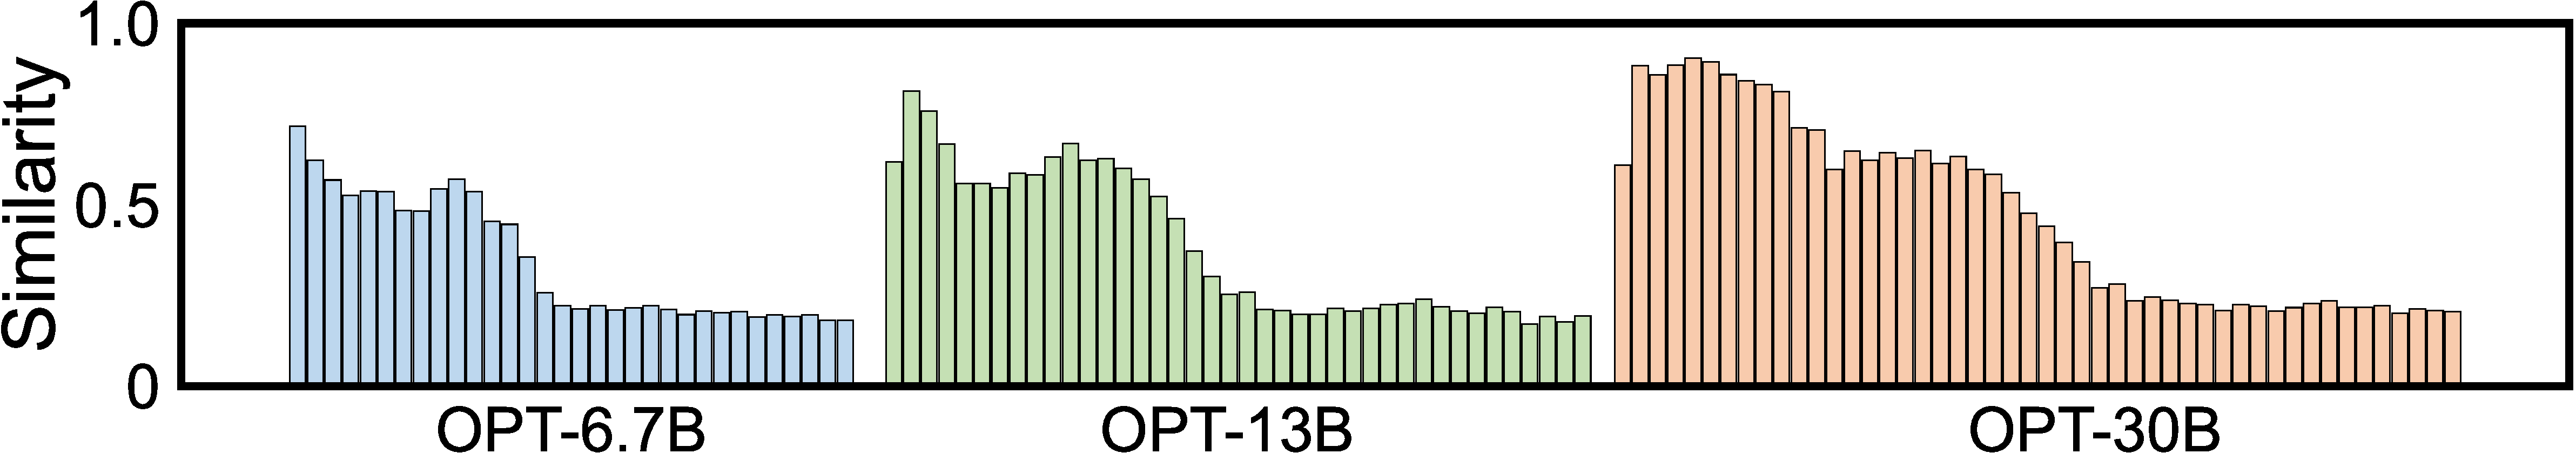
\includegraphics[width=3.2in, height=0.6in]{sim-ten.pdf}
%	}
%	\subfigure[select the top 40\% most important tokens]{
%		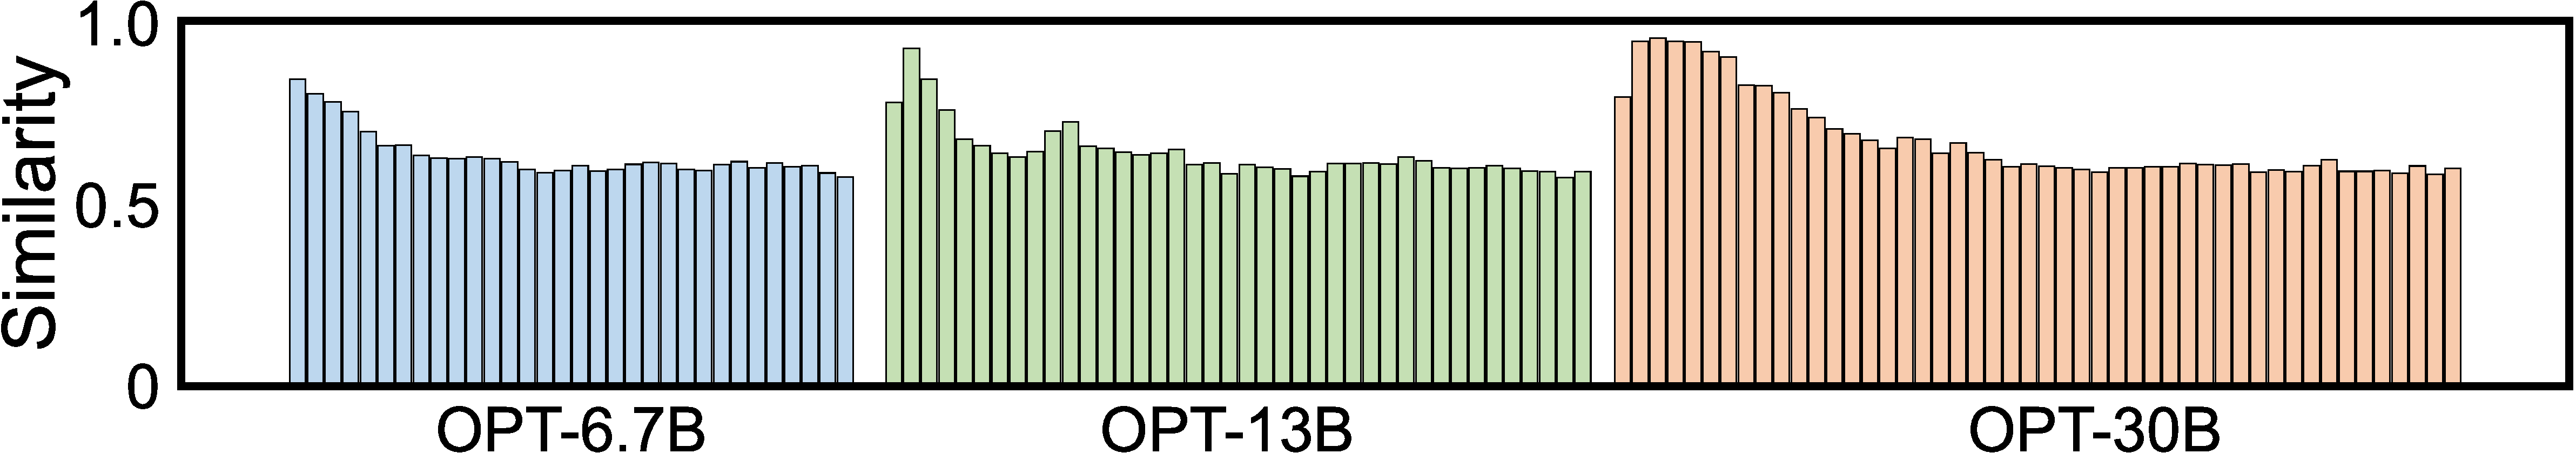
\includegraphics[width=3.2in, height=0.6in]{sim-forty.pdf}
%	}
%	\vspace{-0.1in}
%	\caption{Similarities of important token index sets across all transformer layers.}
%	\label{fig:simi-values}
%	\vspace{-0.1in}
%\end{figure}
%
%%This observation holds across different sampling ratios and LLM scales.
%%For example, Figure~\ref{} shows that as the proportion of important tokens selected varies from 10\% to 100\%, the average similarity across all layers of the OPT-30B model exceeds xx for a randomly selected request from the xx dataset. Figure~\ref{} shows that the average similarity across all layers of the OPT models, ranging from 1.3B to 30B, is consistently greater than x.
%%when the proportion of important tokens is set to xx, 
%
%%\vspace{-1.0ex}
%%\begin{framed}
%%\vspace{-1.2ex}
%%\noindent
%%\textbf{Observation II:}{
%%The similarity of important tokens (represented as important token index sets) exists across different sampling ratios and LLM scales.
%%}
%%\end{framed}
%\noindent
%\textbf{Observation II:}{
%	The similarity of important tokens (represented as important token index sets) exists across different sampling ratios and LLM scales.
%}
%
%To gain further insights, we study the average similarity of token index sets across different heads for the OPT-6.7B, OPT-13B, and OPT-30B models,
%%\ysl{This analysis focuses on scenarios where the top 10\% and 40\% of the most critical tokens were selected, as illustrated in Figure~\ref{fig:simi-values}.}
%when selecting the top 10\% and 40\%  most important tokens (Figure~\ref{fig:simi-values}). 
%Each bar in the figure represents the average value for a single transformer
%layer. These three models contain a total of 32, 40, and 48 transformer layers,
%respectively. We have two findings.
%(1) The higher ratio of important tokens selected, the greater the similarity. For instance, when selecting 40\% and 10\% of the tokens, the average similarity across all layers of OPT-30B is 0.68 and 0.48, respectively. This aligns with intuition, as the similarity reaches 1 when all the tokens (100\%) are selected. 
%(2) Although smaller models and deeper transformer layers tend to exhibit lower similarities, they are still significantly higher than the expected value from random selection in most cases. 
%%For example, while the last layer of OPT-6.7B has a similarity value of only 0.18 when selecting the top 10\% important tokens, the expected similarity from randomly selecting 10\% of tokens is merely \( 10\% / (2 - 10\%) \approx 0.053 \). 
%%This indicates that the observation does indeed hold across different models and layers, even if it is sometimes less pronounced.
%%(2) Larger models tend to exhibit higher similarity. For example, when selecting 50\% of the tokens, the average similarity across all layers of OPT-30B and OPT-6.7B is xx and yy, respectively. This could be attributed to the stronger inference capabilities of larger models, which result in more distinct differences between the vector representations of important and unimportant tokens, leading to more consistent important token index sets across different heads.
%%(3) Within the same model, deeper transformer layers tend to have lower similarity compared to shallower ones. This may be because shallower transformer layers focus on extracting specific features from tokens, while deeper blocks capture more complex relationships between tokens, causing greater variation in the important tokens identified by different heads.
%
%
%
%%\textbf{Observation 2:} \textit{.}
%\noindent
%\zrdnew{
%\textbf{Observation III: }
%{Important token indices also exhibit strong consistency across adjacent layers of an LLM}
%}
%
%xxx

\subsection{\techA{}}

\label{sec:techa}

\begin{figure}
	\centering
	\subfigure[Two Heads of K Tensors]{
		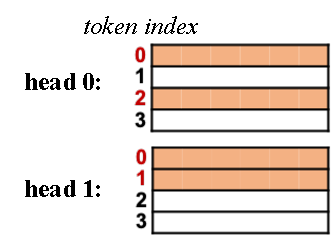
\includegraphics[width=1.5in, height=1in]{jcd-example.pdf}
		\label{fig:jcd-example}
	}
	\hspace{0.06in}
	\subfigure[Jaccard Scores Between Heads]{
		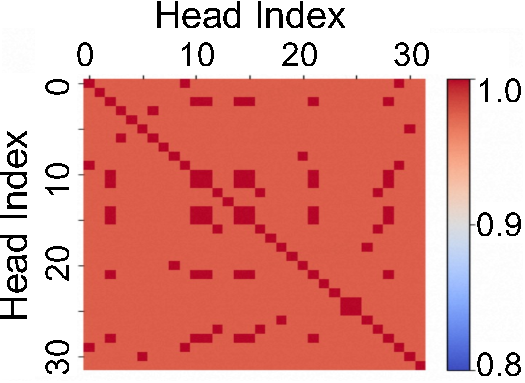
\includegraphics[width=1.5in, height=1in]{real-jcd-example.pdf}
		\label{fig:real-jcd-example}
	}
	\vspace{-0.1in}
	\caption{Examples of similarities. (a) The orange rows represent the important keys whose token indices are marked in red. (b) Darker squares indicate a higher similarity between the important token index sets of two heads.}
	\vspace{-0.1in}
\end{figure}



%We highlight two key observations regarding the characteristics of important tokens.
%Although we cannot strictly prove these observations mathematically for all LLMs and scenarios, we demonstrate the generality and practicality of these findings by showing the impact on accuracy when designs based on these observations are applied, across x datasets and x models.
%, we will demonstrate the generality and practicality of these observations through accuracy evaluations after applying the corresponding techniques on x datasets and x models.

%\vspace{-1.0ex}
%\begin{framed}
%\vspace{-1.4ex}
%\noindent
%\textbf{Observation I:}{
	%There is a high similarity in the set of important token indices 
	%across different heads within the same layer of an LLM.
	%}
%\vspace{-1.4ex}
%\end{framed}
\noindent
\textbf{Observation I:}{
	There is a high similarity in the set of important token indices 
	across different heads within the same layer of an LLM.
}

%\textbf{Observation 1.} \textit{There is a high similarity in the set of important token indices across different heads within the same layer.}

As discussed in \cref{sec:llm-basic}, each token has K and V tensors for every head. 
We observe that important token indices are highly similar across heads within the same layer, 
as \(k\) and \(v\) tensors originate from the same large K and V tensors~\cite{alluneed-nips17, opt-arxiv22}. 
Thus, a token important in one head is likely important in others. 
While this cannot be formally proven for all LLMs, its generality and practicality are validated through accuracy evaluations (\cref{exp:overall}) on four datasets across three models.


To quantify the similarity between important token index sets, we use the Jaccard index~\cite{jaccard-18}, defined as 
\( J(A, B) = \frac{|A \cap B|}{|A \cup B|} \),
where \(A\) and \(B\) denote the important token index sets of two heads. 
The value ranges from 0 (completely different) to 1 (identical). 
As shown in Figure~\ref{fig:jcd-example}, for an input with four tokens where 50\% are important, 
\( h_0 = \{0, 2\} \) and \( h_1 = \{0, 1\} \), yielding \( J(h_0, h_1) = \frac{1}{3} \). 
A real similarity heatmap from the middle layer of OPT-6.7B (Figure~\ref{fig:real-jcd-example}) 
shows high similarity among heads, with average values exceeding 0.95.


\begin{figure}
	\centering
	\subfigure[select the top 10\% most important tokens]{
		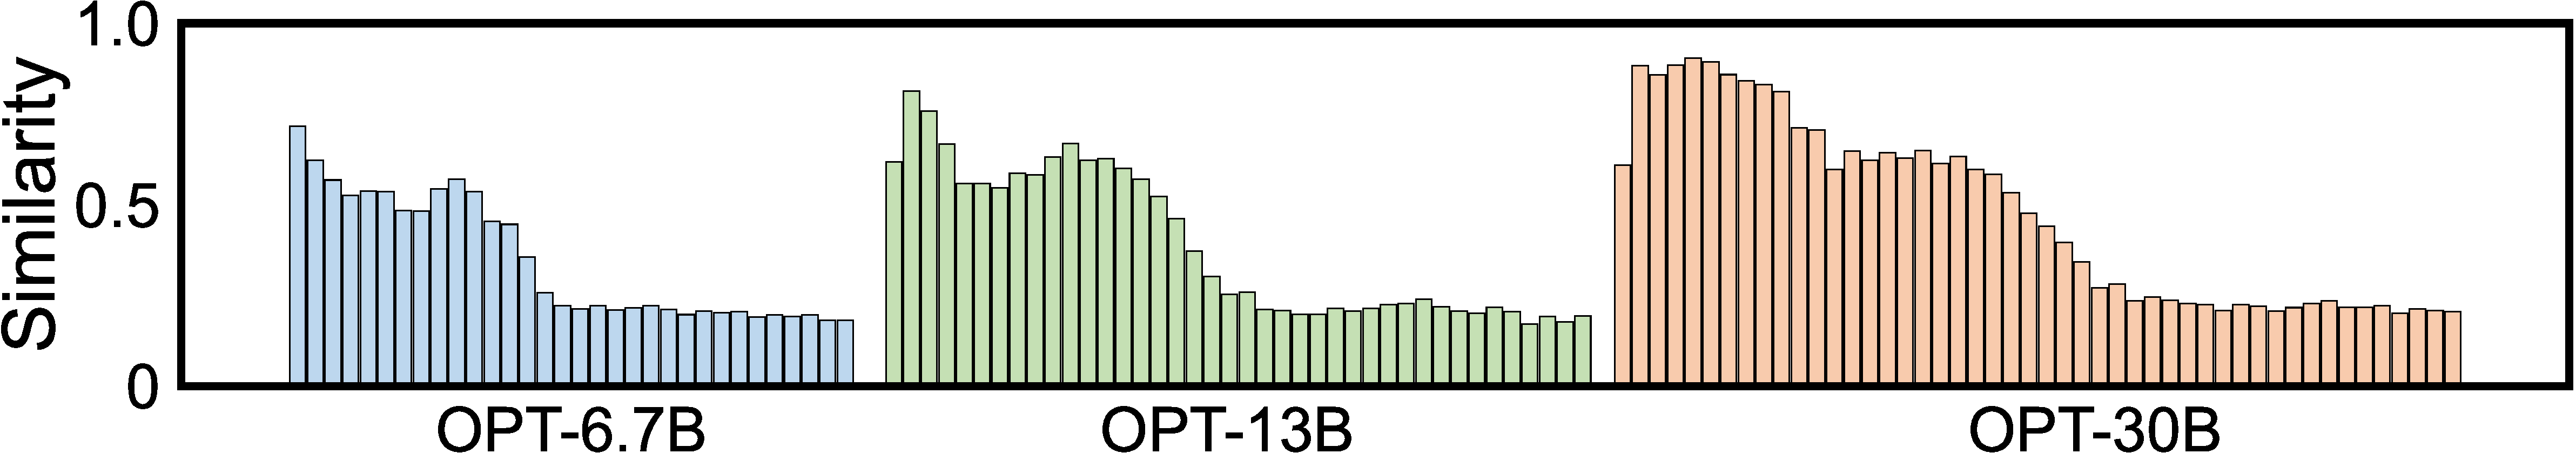
\includegraphics[width=3.2in, height=0.6in]{sim-ten.pdf}
	}
	\subfigure[select the top 40\% most important tokens]{
		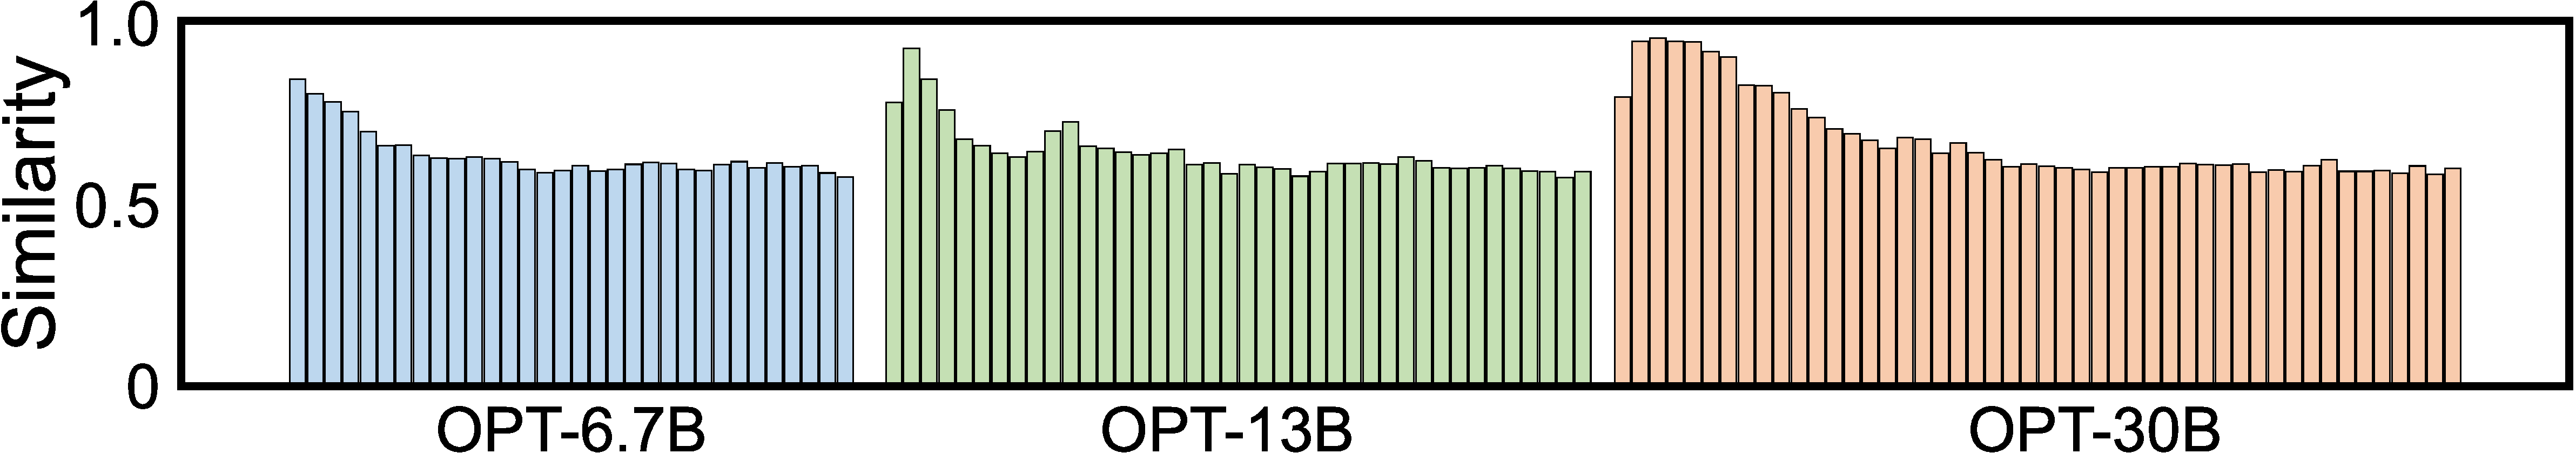
\includegraphics[width=3.2in, height=0.6in]{sim-forty.pdf}
	}
	\vspace{-0.1in}
	\caption{Similarities of important token index sets across all transformer layers.}
	\label{fig:simi-values}
	\vspace{-0.1in}
\end{figure}

%This observation holds across different sampling ratios and LLM scales.
%For example, Figure~\ref{} shows that as the proportion of important tokens selected varies from 10\% to 100\%, the average similarity across all layers of the OPT-30B model exceeds xx for a randomly selected request from the xx dataset. Figure~\ref{} shows that the average similarity across all layers of the OPT models, ranging from 1.3B to 30B, is consistently greater than x.
%when the proportion of important tokens is set to xx, 

%\vspace{-1.0ex}
%\begin{framed}
%\vspace{-1.2ex}
%\noindent
%\textbf{Observation II:}{
	%The similarity of important tokens (represented as important token index sets) exists across different sampling ratios and LLM scales.
	%}
%\end{framed}
\noindent
\textbf{Observation II:}{
	The similarity of important tokens (represented as important token index sets) exists across different sampling ratios and LLM scales.
}

To further understand this phenomenon, we analyze the average similarity of important token index sets across different heads for the OPT-6.7B, OPT-13B, and OPT-30B models when selecting the top 10\% and 40\% most important tokens (Figure~\ref{fig:simi-values}). 
Each bar denotes the average similarity for one transformer layer, with 32, 40, and 48 layers in the three models, respectively. 
We have two findings: 
(1) selecting a larger proportion of important tokens leads to higher similarity. For example, in OPT-30B, the average similarity is 0.68 when selecting 40\% tokens and 0.48 when selecting 10\%, consistent with the intuition that similarity approaches 1 when all tokens are included; 
(2) although smaller models and deeper layers generally show lower similarity, they remain substantially above the random-selection baseline in most cases.

%For example, while the last layer of OPT-6.7B has a similarity value of only 0.18 when selecting the top 10\% important tokens, the expected similarity from randomly selecting 10\% of tokens is merely \( 10\% / (2 - 10\%) \approx 0.053 \). 
%This indicates that the observation does indeed hold across different models and layers, even if it is sometimes less pronounced.
%(2) Larger models tend to exhibit higher similarity. For example, when selecting 50\% of the tokens, the average similarity across all layers of OPT-30B and OPT-6.7B is xx and yy, respectively. This could be attributed to the stronger inference capabilities of larger models, which result in more distinct differences between the vector representations of important and unimportant tokens, leading to more consistent important token index sets across different heads.
%(3) Within the same model, deeper transformer layers tend to have lower similarity compared to shallower ones. This may be because shallower transformer layers focus on extracting specific features from tokens, while deeper blocks capture more complex relationships between tokens, causing greater variation in the important tokens identified by different heads.



%\textbf{Observation 2:} \textit{.}

\textbf{Design}. Based on the above observations, we propose the \techa{} technique. The core idea is that \textit{because of the similarity we can leverage the important token index set generated from a few selected heads to approximate the important token index sets for the remaining heads}. For simplicity, we refer to these selected heads as \textit{probe heads}. Since this process involves loading only keys from a subset of the heads instead of all heads, it reduces both I/O data volume and TTFT.

As some layers exhibit less pronounced similarity between important token
sets across different heads, applying this technique to these layers may
misidentify important tokens in some heads, reducing the model's
inference accuracy. To tackle this issue, we introduce a similarity threshold
that dynamically determines whether to apply the technique
for each transformer layer.
The \techa{} is enabled only when the measured similarity value from the probe heads 
is higher than the similarity threshold.

\begin{figure}
	\centering
	\subfigure[w/o similarity-guided token selection]{
		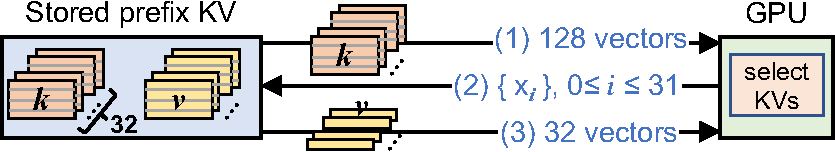
\includegraphics[width=3.2in, height=0.6in]{wo-techa.pdf}
	}
	\subfigure[w/ similarity-guided token selection]{
		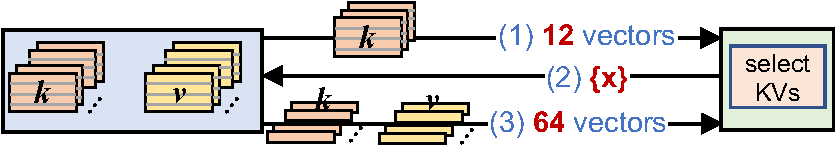
\includegraphics[width=3.2in, height=0.6in]{w-techa.pdf}
	}
	\vspace{-0.1in}
	\caption{The process of transformer layer computation with prefix kv. Each \(k\) and \(v\) tensor has four row vectors because of four tokens in the prefix.}
	\label{fig:woandw-techa}
	\vspace{-0.1in}
\end{figure}



\zrd{Figure~\ref{fig:woandw-techa} illustrates the process of completing a transformer layer with and without this technique. Assume the prefix contains 4 tokens, with only one being important. Each transformer layer has 32 heads and all the prefix KVs of each head are stored on disk. The number of probe heads is set to three. 
Without it, all 32 heads must load 128 key vectors and later 32 \(k,v\) vectors, totaling 160 vectors. 
With \techa{}, only 12 key vectors from three probe heads are first loaded. The GPU computes attention and measures probe-head similarity. 
If the similarity exceeds the threshold, only one token index deemed most important by all probe heads \(\{x\}\) is used, and 64 \(k,v\) vectors are loaded---just 76 vectors in total. 
When the threshold is unmet, the process reverts to the standard mode, though this occurs in fewer than 20\% of layers. 
Given that modern LLMs have dozens of heads and long prefixes, \techa{} effectively reduces I/O load across most layers. }
%Figure~\ref{fig:woandw-techa} illustrates the process of completing a transformer layer with and without this technique. Assume the prefix contains 4 tokens, with only one being important. Each transformer layer has 32 heads and all the prefix KVs of each head are stored on disk. The number of probe heads is set to three. 
%Without the \techa{} technique, it involves three steps: 
%(1) loading the keys of all 32 heads (total 32 $\times$ 4 = 128 vectors) from
%disk into the GPU memory; 
%(2) GPU calculates attention weights using the query and all the keys,
%identifies the most important token index in each head \( i \): $\{x_i\}, \ 0
%\leq i \leq 31$, and returns them to the CPU memory; The detailed identification
%algorithm is based on H2O~\cite{h2o-nips23}.
%(3) The CPU then loads the \(k\) and \(v\) vectors of $\{x_i\}$ from each head
%(total 32 $\times$ 1 = 32 vectors) into the GPU memory to complete the remaining
%prefill computations. The entire process loads a total of 128 + 32 = 160
%vectors.
%
%In contrast, with the \techa{} technique, the steps are as follows:
%(1) only the keys from the three probe heads (total 3 $\times$ 4 = 12 vectors)
%are loaded from disk into the GPU memory; 
%(2) GPU calculates attention weights using the query and the keys from the probe heads, 
%identifies the important token index sets of the three heads, 
%and computes the average Jaccard similarity. 
%If this similarity exceeds the similarity threshold, only one token index 
%deemed most important by all probe heads, $\{x\}$, are returned to the CPU; Then, proceed to step (3).
%If the threshold is not met, the computation mode of the current layer falls back to the version without enabling the \techa{} method.
%(3) The CPU then loads the \(k\) and \(v\) vectors of $\{x\}$ from each head
%(total 32 $\times$ 1 $\times$ 2 = 64 vectors) into the GPU  memory for the remaining
%computations. The entire process loads a total of 12 + 64 = 76 vectors.
%While the I/O data volume cannot be reduced when the probe heads' similarity does not exceed the threshold, this situation only occurs in less than 20\% transformer layers in the \pname{} system on average (see \cref{exp:indiv}). Moreover, in practical LLM models, each transformer layer typically has dozens of heads (e.g., 32-96 in various sizes of the OPT model) and the prefix contains thousands of tokens~\cite{chunkattention-arxiv24, cachegen-sigcomm24}, making this technique effective in reducing I/O data volume across the entire model.
%

\begin{figure}
	\centering
	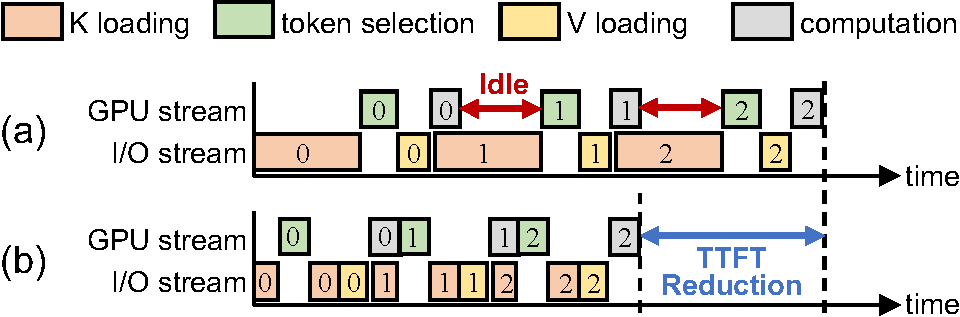
\includegraphics[width=3.4in, height=1.2in]{simiload-ttft.pdf}
	\caption{The TTFTs with and without \techa{}. Assume the LLM model consists of three transformer layers. The numbers inside the rectangles represent the layer index.}
	\label{fig:simiload-ttft}
\end{figure}


Figure~\ref{fig:simiload-ttft} compares the timeline for completing three transformer layers with and without this technique. 
Without \techa{}, in Figure~\ref{fig:simiload-ttft}(a), the loading of a large number of keys leads to GPU idle time, prolonging inference process. In contrast, when the technique is enabled in Figure~\ref{fig:simiload-ttft}(b), and the probe heads’ similarity exceeds the threshold, the time required to load only the keys from the probe heads (in red color) is significantly shorter, thereby reducing GPU wait time. Additionally, loading only a subset of keys for attention weight calculations reduces the time spent generating important token index sets (in green color), leading to a shorter overall TTFT.

\noindent \textbf{Hyperparameter decisions.}
%To make this algorithm practical, we need to determine the number of probe heads and the similarity threshold.
%Selecting only one probe head to determine the most important token index may introduce bias, affecting model accuracy. Using two probe heads might fail to identify the most important index through voting when disagreements arise. Therefore, we choose to use three probe heads. Increasing the number of probe heads offers minimal improvements in accuracy but increases the keys loading time, thereby extending the TTFT.
%Additionally, we found that the choice of which three heads to use has no impact on accuracy due to the similarity. 
%Therefore, we simply select the first three heads in each transformer layer as the probe heads to keep the selection process quick.
%\fv{
%We first compute the similarity of important token sets between each pair of  probe heads, and then take the average to measure the overall similarity among the three probe heads. Thus, the similarity is independent of the order of probe heads.
%}
\zrd{To make the algorithm practical, we need to determine the number of probe heads and the similarity threshold. Using a single probe head may introduce bias, while two heads can yield inconsistent voting results. We therefore adopt three probe heads, which balance accuracy and efficiency. Adding more heads provides negligible accuracy gains but increases key-loading latency and TTFT. Since the choice of heads has minimal effect due to their high similarity, we simply use the first three heads in each transformer layer for fast selection. 
}


\begin{figure}
	\centering
	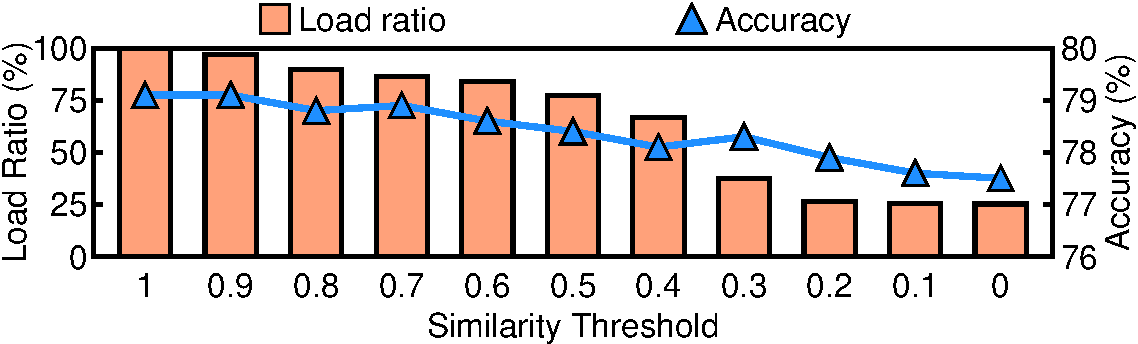
\includegraphics[width=3.3in, height=1in]{dif_sim_thred.pdf}
	\vspace{-0.1in}
	\caption{
		The proportion of keys loaded and the model inference accuracy under different similarity thresholds.}
	\label{fig:thred}
	\vspace{-0.1in}
\end{figure}


% Determining the similarity threshold is not trivial. A threshold that is too high may result in not reducing the number of keys and values in many transformer layers because the average similarity of the probe heads is consistently below the threshold. Conversely, a threshold that is too low can lead to biased results in the identified important token index set, thereby degrading model accuracy. 
% Figure~\ref{fig:thred} shows an example on the PIQA~\cite{lmeval} dataset, where we set each transformer layer to select 25\% of the most important prefix KVs. Although lowering the threshold from 1 to 0 reduces the number of keys loaded by 4$\times$, it also causes a drop in accuracy from 79.1\% to 77.5\%.
% Similar trends are observed on other datasets.

%Setting the similarity threshold is complex. A threshold set too high might fail to reduce the number of keys and values across many transformer layers, as the average similarity of the probe heads often falls short of the threshold. On the other hand, a threshold set too low can introduce bias in the identified important token index set, compromising model accuracy.
%Figure~\ref{fig:thred} illustrates this on the PIQA~\cite{lmeval} dataset, where each transformer layer selects the top 25\% of the most critical prefix KVs. Although decreasing the threshold from 1 to 0 cuts the number of keys loaded by 4$\times$, it also results in a 1.6\% decrease in accuracy, from 79.1\% to 77.5\%. Similar patterns are observed across other datasets.
%
%
%To address this issue, we first calculate the expected value based on the proportion of selected important tokens, then slightly increase this value and use it as the similarity threshold.
%Specifically, suppose we have a prefix containing \(n\) tokens and need to select \(k\) important tokens (\(k \leq n\)). If we randomly execute this selection twice, we obtain sets \(A\) and \(B\). The probability of each token appearing in both sets is \(\frac{k^2}{n^2}\). Given \(N\) tokens in total, \(E(A \cap B) = n \cdot \frac{k^2}{n^2}\ = \frac{k^2}{n}\), and \(E(A \cup B) = E(A) + E(B) - E(A \cap B) = k + k - \frac{k^2}{n} = 2k - \frac{k^2}{n}\). Therefore, \(E(\text{Jaccard}(A, B)) = \frac{E(A \cap B)}{E(A \cup B)} = \frac{k/n}{2 - (k/n)}\). Denote this expected value as \(j\). We set the threshold \(t = j^\alpha\), where we empirically choose \(\alpha = 0.6\) in our experiments to achieve a good balance between model inference accuracy and the amount of keys loaded. 
\zrd{Setting the similarity threshold requires careful balance. A threshold that is too high prevents key–value reduction across layers, while one that is too low biases the important-token selection and harms accuracy. As shown in Figure \ref{fig:thred} on the PIQA \cite{lmeval} dataset, lowering the threshold from 1 to 0 reduces key loading by 4× but decreases accuracy by 1.6 points (79.1% → 77.5%), with similar trends across other datasets.
To mitigate this, we estimate the expected Jaccard similarity between two random selections of $k$ important tokens from $n$ candidates as $E(\text{Jaccard}) = \frac{k/n}{2 - (k/n)}$, denoted by $j$, and set the threshold to $t = j^{\alpha}$. Empirically, choosing $\alpha = 0.6$ provides a good trade-off between inference accuracy and the number of loaded keys.
\zrd{Setting the similarity threshold is crucial. 
	A high threshold may fail to reduce key-value loading, as probe head similarity often falls below it; 
	a low threshold, however, can bias the selected important tokens and degrade accuracy. 
	As shown in Figure~\ref{fig:thred} on the PIQA~\cite{lmeval} dataset, each transformer layer selects the top 25\% most critical prefix KVs. 
	Lowering the threshold from 1 to 0 reduces the number of loaded keys by 4$\times$, but also decreases accuracy from 79.1\% to 77.5\%. 
	Similar trends hold across other datasets.
}


To address this issue, we first calculate the expected value based on the proportion of selected important tokens, then slightly increase this value and use it as the similarity threshold.
Specifically, suppose we have a prefix containing \(n\) tokens and need to select \(k\) important tokens (\(k \leq n\)). If we randomly execute this selection twice, we obtain sets \(A\) and \(B\). The probability of each token appearing in both sets is \(\frac{k^2}{n^2}\). Given \(N\) tokens in total, \(E(A \cap B) = n \cdot \frac{k^2}{n^2}\ = \frac{k^2}{n}\), and \(E(A \cup B) = E(A) + E(B) - E(A \cap B) = k + k - \frac{k^2}{n} = 2k - \frac{k^2}{n}\). Therefore, \(E(\text{Jaccard}(A, B)) = \frac{E(A \cap B)}{E(A \cup B)} = \frac{k/n}{2 - (k/n)}\). Denote this expected value as \(j\). We set the threshold \(t = j^\alpha\), where we empirically choose \(\alpha = 0.6\) in our experiments to achieve a good balance between model inference accuracy and the amount of keys loaded. 
%\zrd{Setting the similarity threshold requires careful balance. A threshold that is too high prevents key–value reduction across layers, while one that is too low biases the important-token selection and harms accuracy. As shown in Figure \ref{fig\:thred} on the PIQA \cite{lmeval} dataset, lowering the threshold from 1 to 0 reduces key loading by 4× but decreases accuracy by 1.6 points (79.1% → 77.5%), with similar trends across other datasets.
%	To mitigate this, we estimate the expected Jaccard similarity between two random selections of $k$ important tokens from $n$ candidates as $E(\text{Jaccard}) = \frac{k/n}{2 - (k/n)}$, denoted by $j$, and set the threshold to $t = j^{\alpha}$. Empirically, choosing $\alpha = 0.6$ provides a good trade-off between inference accuracy and the number of loaded keys.
%}




%\textbf{\techAa{}}

\subsection{\techNew{}}
\label{sec:techc}
% \subsection{Data Locality in Micrographs}
\label{sec:technew}

%基于
\noindent
\zrdnew{
	\textbf{Observation III: }
	{Important token indices exhibit strong consistency across adjacent layers of an LLM.} To further analyze the distribution of important token indices, we examine the similarity of the top 25\% important token sets across adjacent layers for different models. As shown in Figure~\ref{fig:ob3}(a), there are two key observations: (1) the important tokens exhibit strong consistency across layers, and (2) tokens with higher importance in one layer are more likely to remain important in the subsequent layer.
	Specifically, xxxx.}
% 把图中的一些趋势或者例子挑出来说一下。

%
\begin{figure}
	\centering
	\subfigure[select the top 25\% most important tokens]{
		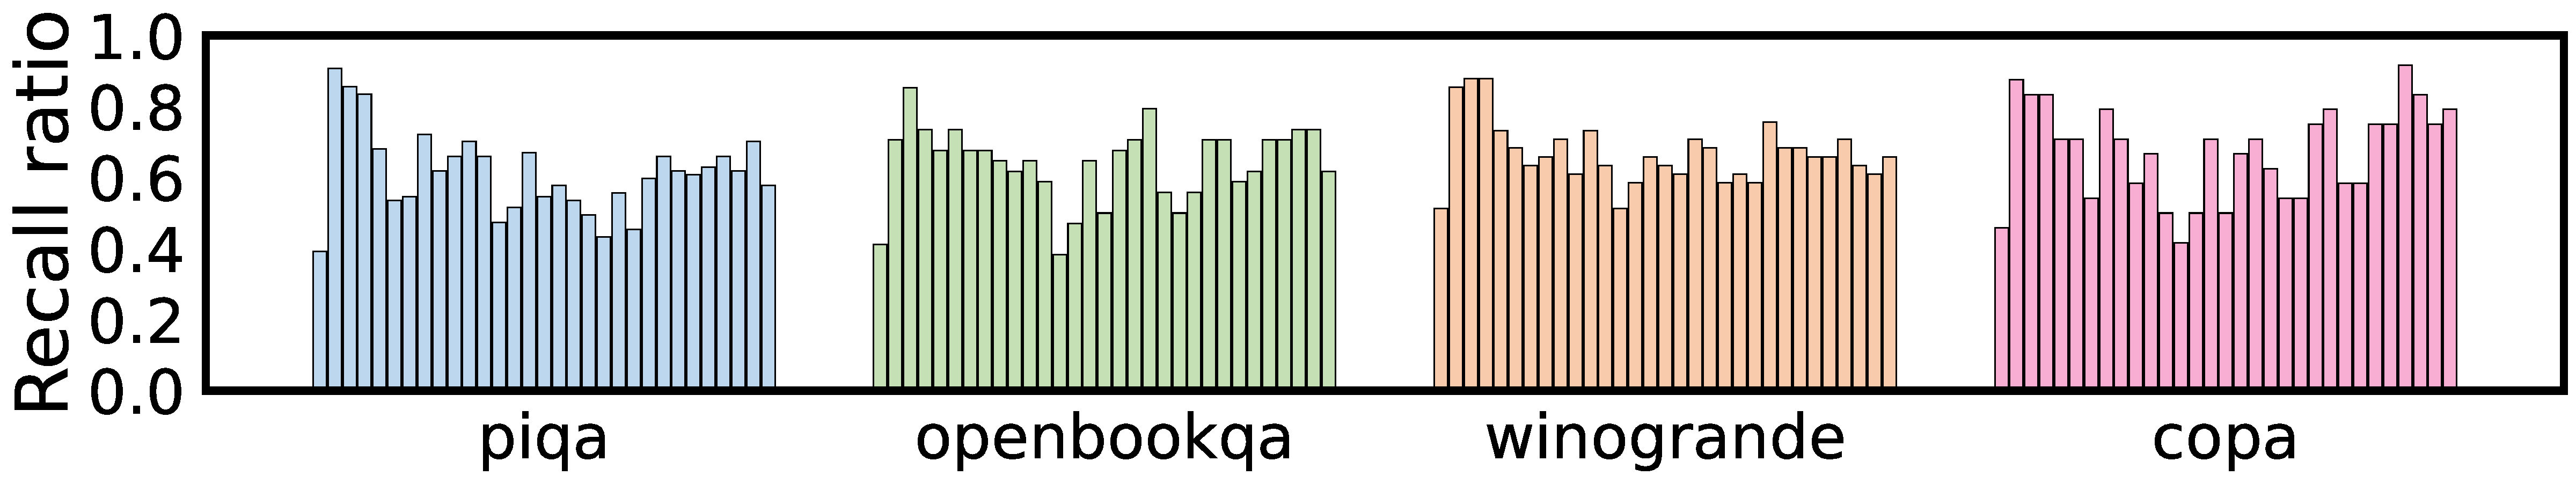
\includegraphics[width=1.5in, height=1in]{sim-25-cross-layers.pdf}
	}
	\subfigure[select different percentage most important tokens]{
		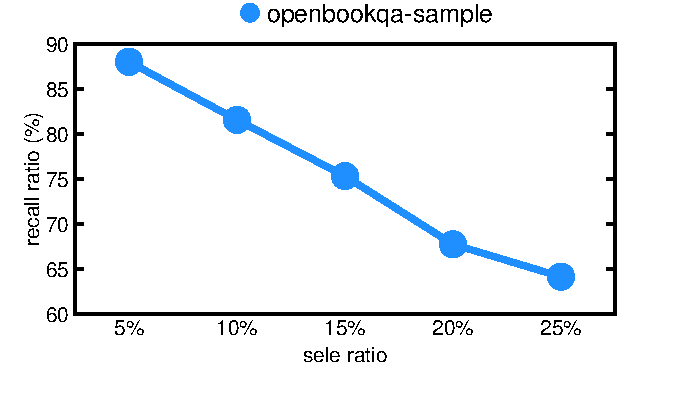
\includegraphics[width=1.5in, height=1in]{recall-sele.pdf}
	}
	\vspace{-0.1in}
	\caption{Similarities of important token index sets of adjacent layers.}
	\label{fig:ob3}
	\vspace{-0.1in}
\end{figure}
%如图xx所示,在模型的一层内,识别重要token index set和加载重要token的kv是有数据依赖的,在没有识别得到重要token index set的情况下,我们无法准确预取下一层所需的重要kv,因此在此层计算时,宝贵的I/O带宽没有被利用,在一个本就I/O瓶颈的场景下。一个naive的方法是,随机的预取一些下一层可能用到的token的kvs到GPU memory中,在下一层的重要token选择完成后,再把不在gpu mem的重要kv load到gpu mem中,然而这样的方法受制于完全不知道下一层重要token index的分布,准确率差,浪费了I/O带宽。一些工作提出了attention sink的概念,即一些特定位置的token在推理过程中总是重要的,如prompt的开头和结尾的几个token,然而,仅预取sink位置的token准确率仍不一定高(一些引用),且存在带宽利用不充分的可能。因此我们提出一种准确率高,灵活的指导预取的方法,高效的预取下一层的重要kv,并将预取与计算overlap起来。我们study了\cref{sec:techa}中提到的识别重要token的方法所识别出的重要token,发现在模型的相邻层重要token的分布是相似的,且重要性排名分位越靠前的index集合,相似度越高。相似度仍用jaccard index量化。
%图片xx描述了基于相似性的重要token识别方法识别出的,图片xx

%\zrdnew{For the important tokens identified as shown in Figure xx, within a given layer of the model, there exists a data dependency between identifying the important token index set and loading the corresponding prefix KVs. Without first identifying the important token index set, we are unable to accurately prefetch the necessary KVs for the next layer. As a result, valuable I/O bandwidth remains underutilized during computation in a scenario that is already constrained by I/O bottlenecks. A naive approach would be to randomly prefetch some potential KVs for the next layer into GPU memory. After the important token selection for the next layer is completed, any important KVs not already in GPU memory can then be loaded into it. However, this approach suffers from the challenge of not knowing the distribution of the important token index set for the next layer, resulting in low accuracy and wasted I/O bandwidth. Some works have proposed the concept of attention sinks, where certain tokens at specific positions, such as the beginning and end of a prompt, are always important during inference. However, prefetching only these sink tokens may still result in low accuracy (some references), and there is a risk of inefficient bandwidth utilization.}
%
%\zrdnew{To address these issues, we propose a more accurate and flexible guidance-based prefetching method that efficiently prefetches important KVs for the next layer while overlapping prefetching with computation. We studied the important tokens identified by the method mentioned in \cref{sec:techa} and found that the distribution of important tokens in adjacent layers is highly similar. Moreover, the index sets with higher importance rankings exhibit higher similarity. This similarity is quantified using the Jaccard index.}

\cp{
Loading important KVs during inference lies on the critical path and thus introduces non-negligible latency, as shown in Figure~\ref{}. 
To alleviate this overhead, we explore using prefetching to hide the I/O cost by overlapping data loading with computation. 
However, this presents a key challenge: the important tokens for the next transformer layer are unknown until the current layer’s computation completes, making it difficult to determine which KVs to prefetch in advance. 
To solve this challenge, based on \textit{Observation~III}, we propose the \technew{} mechanism, which exploits the strong similarity of important token index sets across adjacent layers. 
During the computation of the current layer, \technew{} asynchronously prefetches the important KVs of the next layer into GPU memory by approximating the next layer’s important tokens with those identified in the current layer. 
This layer-aware prefetching effectively reduces I/O latency and achieves higher accuracy than random prefetching.}


Existing LLM serving systems often face high inference latency due to inefficient KV management across GPU, CPU, and disk. 
Only KVs stored in GPU memory can be accessed with low latency, while fetching KVs from CPU or disk introduces substantial delay. 
These data transfers frequently occur on the critical path, causing I/O stalls, bandwidth underutilization, and longer time-to-first-token (TTFT). 


To address these issues, we propose an \textbf{importance-informed key–value (KV) prefetching system} with a \textbf{Dual Budget Strategy (DBS)} that jointly optimizes computation and I/O efficiency across heterogeneous storage tiers. 
Instead of merely overlapping data transfer with computation, our approach dynamically determines \emph{which} KVs to load and \emph{how much} I/O time to allocate to each storage tier within a fixed computation window $T_{\text{comp}}$. 
During each iteration, DBS prioritizes the KVs that yield the greatest accuracy improvement per unit of I/O cost and allocates separate time budgets for disk reads and PCIe transfers, ensuring that prefetching proceeds efficiently without exceeding the computational critical path.

Our system comprises two key components: (1) \textbf{importance-aware token prioritization} and (2) \textbf{dual-stage time budgeting}.  
First, each token is assigned an importance score $v(t)$ derived from its attention weight, while the cost of loading it from storage is estimated as $c(t) = c_{\text{disk}}(t) + c_{\text{pcie}}(t)$.  
We compute the ratio $\text{Density}(t) = v(t)/c(t)$ to evaluate how much benefit each unit of I/O time provides and greedily load tokens with the highest densities.  

Second, DBS partitions the computation time $T_{\text{comp}}$ into a disk I/O budget $T_{\text{disk}} = \rho_{\text{disk}}T_{\text{comp}}$ and a PCIe transfer budget $T_{\text{pcie}} = \rho_{\text{pcie}}T_{\text{comp}}$.  
Data are prefetched in a pipeline from disk to CPU and then to GPU, with dynamic budget adjustment to balance both stages and avoid idle time.  
Cached tokens incur negligible cost, while each disk access amortizes latency across multiple tokens, promoting sequential reads and improving throughput.  

Overall, this design minimizes redundant transfers, maximizes bandwidth utilization, and aligns prefetching time with computation, effectively reducing time-to-first-token (TTFT) without sacrificing inference accuracy.



	
%	Based on observation III, we propose the \technew{} mechanism.
%During the computation of the current layer, we  asynchronously prefetch important KVs of the next layer into GPU memory. This prefetching leverages the similarity of important token index sets across layers to improve prefetching accuracy. By approximating the important token index set of the next layer with the set from the current layer, we increase the accuracy of prefetching, leading to better performance compared to random prefetching. Once the important token index set for the next layer is identified, any important tokens' KVs that were not prefetched are then loaded into GPU memory for inference.


\zrdnew{To minimize inference latency in large language models (LLMs), we propose an importance-informed KV prefetching system that integrates a Dual Budget Strategy (DBS) to balance computation and I/O costs across heterogeneous storage tiers. During inference, key-value (KV) pairs are distributed among GPU, CPU, and disk, and the challenge lies in efficiently transferring the most important KVs to the GPU within a fixed computation time $T_{\text{comp}}$. Our design introduces two synergistic components: (1) **importance-aware token prioritization** and (2) **dual-stage time budgeting**. First, we quantify the importance of each token using the attention-based scores from the current layer and derive its expected value $v(t)$. The cost of loading a token $t$ from its storage location is estimated as $c(t) = c_{\text{disk}}(t) + c_{\text{pcie}}(t)$, where $c_{\text{disk}}(t) = \text{size(chunk)}/B_{\text{disk}}$ and $c_{\text{pcie}}(t) = \text{bytes}(t)/B_{\text{pcie}}$ represent the disk-read and PCIe-transfer times respectively. We then compute the **marginal density** $\text{Density}(t) = v(t)/c(t)$ and greedily select tokens with the highest density, ensuring that each unit of I/O time yields maximal contribution to model accuracy. Second, to achieve precise overlap between I/O and computation, we split the total time budget $T_{\text{comp}}$ into a **disk I/O budget** $T_{\text{disk}} = \rho_{\text{disk}}T_{\text{comp}}$ and a **PCIe transfer budget** $T_{\text{pcie}} = \rho_{\text{pcie}}T_{\text{comp}}$, where $\rho_{\text{disk}}$ and $\rho_{\text{pcie}}$ control the relative proportions of disk and PCIe utilization. Within each iteration, data are prefetched from disk to CPU and from CPU to GPU in a pipelined fashion, and dynamic adjustment of both budgets ensures that neither channel becomes idle or exceeds the computational critical path. Tokens already cached in GPU or CPU memory incur zero or partial cost, while the first access to a disk chunk amortizes the full read latency over multiple tokens, naturally encouraging dense, contiguous I/O. This design reduces redundant transfers, maximizes effective bandwidth, and guarantees that the prefetch time closely matches the computation time. The algorithm runs in $O(N\log N)$ time due to sorting by marginal density, with $O(N)$ space complexity. Ablation experiments compare the proposed DBS with static and random prefetching baselines under varying disk and PCIe bandwidths. Each experiment measures the time-to-first-token (TTFT), inference accuracy, and I/O efficiency. Specifically, we vary $\rho_{\text{disk}}$ and $\rho_{\text{pcie}}$ between 0.2 and 0.8 and evaluate scenarios where disk I/O or PCIe becomes the primary bottleneck. Experimental results demonstrate that DBS achieves up to 2.8× reduction in TTFT with negligible accuracy degradation (<0.2\%), confirming that balanced dual-stage budgeting and marginal density–based selection jointly maximize inference throughput under strict time constraints.}

\subsection{Importance-Informed KV Placement}
\label{sec:techb}

\subsubsection{\techBa{}}
\label{sec:techba}
% We propose the \techba{} technique to address the issue where unimportant KVs within the same chunk are also loaded and cached when retrieving important KVs. The core idea is to increase the density of important KVs within a chunk by reordering and repacking them into new chunks, thereby reducing bandwidth waste during reads. 
% This reordering and repacking process is performed periodically \wj{(e.g., 10 minutes in our settings)}, based on the average importance of each token throughout the cycle.
% The entire process is executed asynchronously, so the time spent does not impact the main I/O path.

% We introduce the \techba{} method to tackle the problem of loading and caching unimportant KVs alongside important ones within the same chunk. The essence is to enhance the concentration of important KVs in a chunk by periodically reordering and consolidating them into new chunks, which minimizes bandwidth wastage during read operations.
% This reorganization and repacking is scheduled at regular intervals (e.g., every 10 minutes in our configuration), aligned with the average importance of each token over the cycle. The entire operation is conducted asynchronously, ensuring that the time invested does not interfere with the primary I/O operations.

We present the \techba{} method to address the unnecessary loading of unimportant KVs during important KV retrieval. By periodically reorganizing and repacking important KVs into denser chunks, this approach optimizes read efficiency and reduces bandwidth waste.
Scheduled at regular intervals (e.g., every 10 minutes), this process is based on the average token importance and operates asynchronously to avoid disrupting the main I/O flow.


\begin{figure}
	\centering
	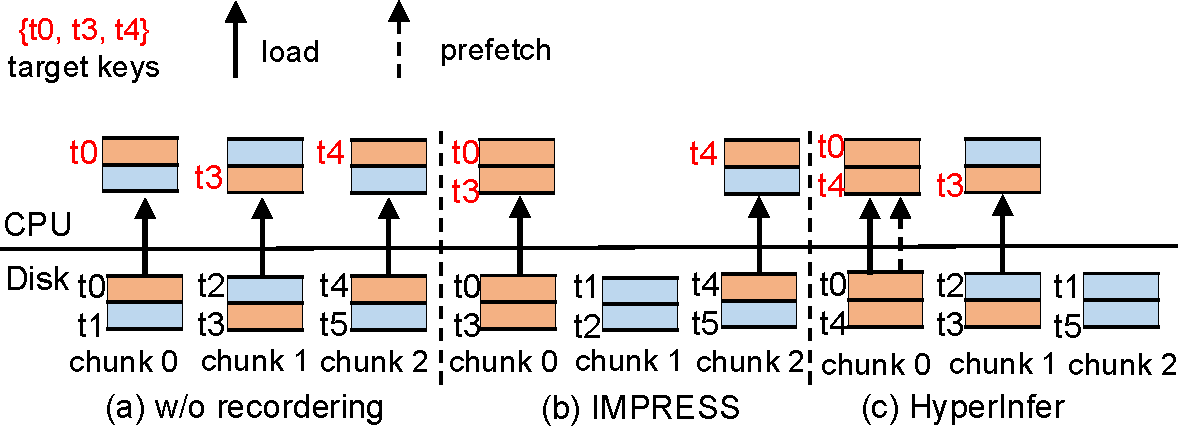
\includegraphics[width=3.4in, height=1.3in]{reorder.pdf}
%	\vspace{-0.1in}
	\caption{Comparison of the number of chunks read before and after the token sequence is reordered. The orange (blue) rectangles represent important (unimportant) keys.}
	\label{fig:reordering}
	\vspace{-0.1in}
\end{figure}

%To illustrate this process, consider an example where a prefix consists of four tokens [t0, t1, t2, t3], and the existing system stores keys for two adjacent tokens in a single chunk. Suppose each chunk contains one important key and one unimportant key.
%Figure~\ref{fig:reordering}(a) demonstrates that, without the \techba{} technique, both chunks must be loaded from disk into CPU memory to retrieve the two important keys \{t0, t3\}. This leads to unimportant keys consuming valuable read bandwidth and cache space. In contrast, with \techba{} enabled (as shown in Figure~\ref{fig:reordering}(b)), the four tokens are first reordered in a descending order of importance, and then the keys of two adjacent reordered tokens (i.e., [t0, t3] and [t1, t2]) are packed into a single chunk. This allows only one chunk to be loaded to access all two important keys, thereby reducing the amount of data read from the disk.
\fvc{
To illustrate, consider a prefix [t0, t1, t2, t3] where the existing system stores keys for two adjacent tokens in one chunk, each containing one important and one unimportant key. Without \techba{} (Figure~\ref{fig:reordering}(a)), both chunks must be loaded to retrieve the important keys \{t0, t3\}, wasting read bandwidth and cache space on unimportant keys. With \techba{} (Figure~\ref{fig:reordering}(b)), tokens are reordered by importance, and keys of adjacent reordered tokens ([t0, t3] and [t1, t2]) are packed into one chunk. This enables loading just one chunk to access all important keys, reducing disk read data.
}

%\noindent \textbf{Metadata adjustment.}
%%In LLM inference, a token's KV can only be reused when that token and all preceding tokens are identical across requests. 
%In LLMs, prefix KVs can only be reused if two prefixes share a common subsequence starting from the first token 
%(i.e., the token order must be the same).
%Therefore, existing systems typically use a radix tree~\cite{sglang-arxiv23, chunkattention-arxiv24} or its variants~\cite{ragcache-arxiv24} to record stored prefix tokens, enabling quick search for reusable stored prefix KVs when a new request arrives. 
%%However, the \techba{} could disrupt the original metadata organization, affecting the ability to check and reuse shared prefix KVs for new requests.
%However, \techba{} may destroy the radix tree structure by altering the token order, 
%causing new requests to fail in locating the correct shared prefix KVs.
%To overcome this, we limit the scope of KV reordering to the tokens within each node of the radix tree. Additionally, we introduce a mapping list within each node to assist the checking operations of new requests.
%We use an example to explain the details.
%
%\begin{figure}
%	\centering
%	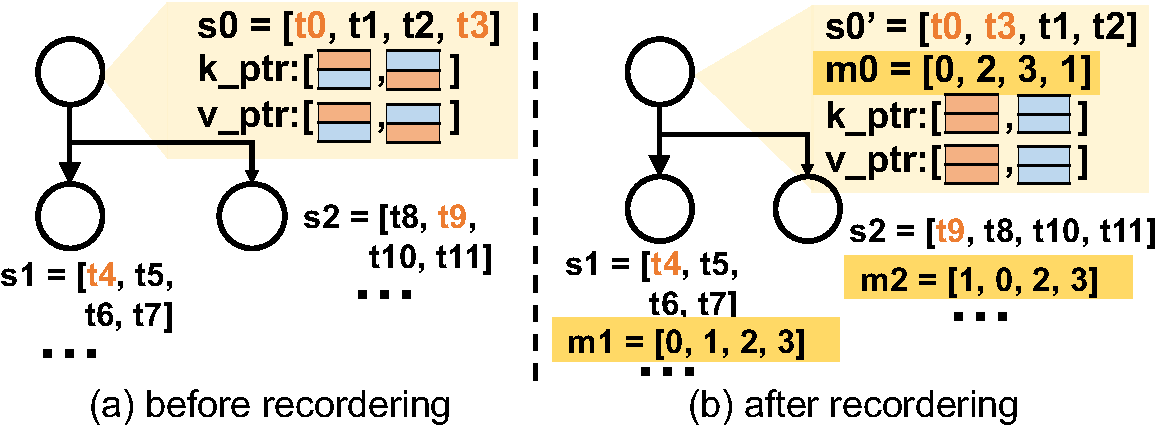
\includegraphics[width=3.3in, height=1.2in]{metaupdate.pdf}
%%	\vspace{-0.1in}
%	\caption{Comparison of meta structure before and after KV reordering. The orange (blue) rectangles represent important (unimportant) keys.}
%	\label{fig:metaupdate}
%	\vspace{-0.1in}
%\end{figure}
%
%Consider two requests that retrieve related document segments as prefixes
%through RAG. Each prefix contains eight tokens: p0=[t0, t1, t2, t3, t4, t5, t6,
%t7] for one request and p1=[t0, t1, t2, t3, t8, t9, t10, t11] for the other. t0,
%t3, t4, and t9 are important data, while the remaining tokens are unimportant.
%Before applying the \techba{} technique, the radix tree is organized as shown in
%Figure~\ref{fig:metaupdate}(a), where the common prefix subsequence s0=[t0, t1,
%t2, t3] is grouped within the same node, enabling the reuse of as many prefix
%KVs as possible. Assume the chunk size is set to 2, with each chunk containing the keys or values of two consecutive tokens.
% Each node contains a list of pointers k\_ptr (v\_ptr) to
%these key (value) chunks.
%
%After enabling \techba{}, as shown in Figure~\ref{fig:metaupdate}(b), the token sequence within each node is reordered in a descending order of importance, and the keys and values are repacked. In Node 0, for example, the token sequence becomes s0' = [t0, t3, t1, t2], with t0 and t3 now grouped within the same chunk. 
%Consequently, reordering disrupts the token sequence in the radix tree.
%We add a new mapping list to Node 0 to address this issue.
%It is denoted as m0 = [0, 2, 3, 1], allowing the original s0 sequence to be recovered using the torch index operation s0'[m0] when search reusable shared prefixes for new requests. This vectorized indexing operation is highly efficient, consuming less than 2\% of the TTFT in our experiments. 
%
%We explicitly avoid cross-node reordering, such as placing t4 and t9 into s0', for two key reasons. First, it would destroy the radix tree structure since t4 and t9 are not common tokens shared by both prefixes (i.e., p0 and p1), potentially leading to errors in retrieving reusable prefix segments for new requests. Second, it would result in unnecessary read bandwidth consumption by loading t9 when reusing the KVs of p0. The constraint against cross-node reordering prevents packing unshared tokens' KVs from different prefixes together, thereby reducing bandwidth wastage.


\subsubsection{\techBb{}}
\label{sec:techbb}
To cut down on PCIe transfers, after loading a chunk from disk into CPU
memory, only the important key and value vectors from that chunk are sent to the
GPU memory via PCIe. However, as depicted in Figure~\ref{fig:imp_token_num}, the
presence of important key or value vectors in a chunk does not align with the
chunk's access frequency. Consequently, existing systems that base their caching
decisions for GPU or CPU memory solely on recency or frequency of chunk access
may lower the GPU cache hit ratio for important key-value pairs, thus increasing
PCIe traffic.

\noindent \textbf{Score-based cache admission.}
To enhance cache efficiency, we introduce the importance-aware cache admission policy.
% \techbb{} policy.
This policy assigns a score to each chunk based on its access frequency and the
proportion of important keys or values it holds. Chunks with higher scores are
preferentially cached in GPU memory, whereas those with lower scores are stored
in CPU memory. This approach boosts the GPU cache hit ratio and minimizes data
transfers between CPU and GPU. The importance ratio is dynamically calculated as
a moving average, updating online after each chunk access.


%\begin{comment}


% For example, assume that key chunk 1 and key chunk 2 come from prefixes requested by application A and application B, respectively, and only one chunk can be stored in the GPU. Since the number of past requests from application A is 1.5 times that of application B, chunk 1 is accessed more frequently than chunk 2. However, only one key (i.e., 50\%) in chunk 1 is important, while both keys (i.e., 100\%) in chunk 2 are important. 
% As shown in Figure~\ref{fig:score_cache}(a), the existing system would place chunk 1 in the GPU and chunk 2 in the CPU because chunk 1 has a higher access frequency. When 15 new requests from application A and 10 new requests from application B arrive, this placement would result in the need to transfer 10 $\times$ 2 = 20 important keys from CPU to GPU. 
% However, considering the importance ratio, chunk 1's score would be 1.5 $\times$ 50\% = 0.75, and chunk 2's score would be 1 $\times$ 100\% = 1. Thus, chunk 2 would be placed in the GPU, as shown in Figure~\ref{fig:score_cache}(b), which would reduce the data transfer during the servicing of the 25 new requests to only 15 $\times$ 1 = 15 important keys.
%\end{comment}

For instance, suppose key chunk 1 from application A and key chunk 2 from
application B are contenders for the limited GPU memory, with application A's
request frequency being 1.5 times that of B, making chunk 1 more frequently
accessed. However, chunk 1 contains only one important key (50\%), while chunk 2
contains two important keys (100\%).
As depicted in Figure~\ref{fig:score_cache}(a), traditional systems would cache
chunk 1 in the GPU memory due to its higher access frequency, relegating chunk 2 to
the CPU. With 15 new requests from A and 10 from B, this approach would
necessitate transferring 20 important keys from CPU to GPU.
By contrast, factoring in the importance ratio, chunk 1 scores 0.75 (1.5 $\times$
50\%), and chunk 2 scores 1 (1 $\times$ 100\%). Thus, our method caches chunk 2 in
the GPU memory, as shown in Figure~\ref{fig:score_cache}(b), cutting the transfer of
important keys to just 15.

\begin{figure}
	\centering
	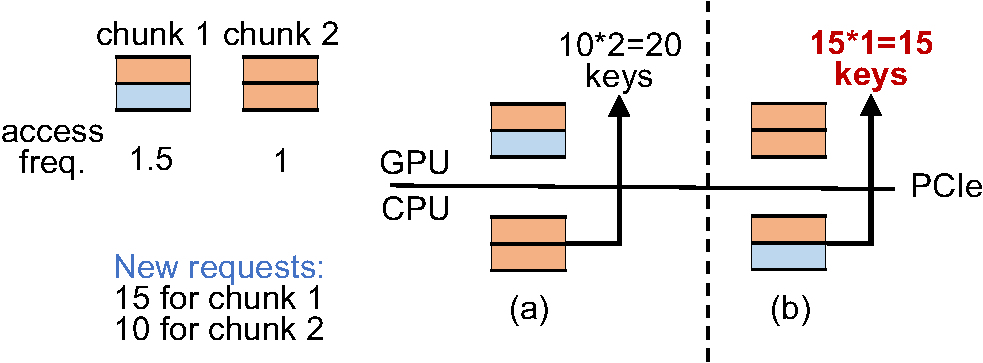
\includegraphics[width=3.3in, height=1.2in]{score_cache.pdf}
	% \vspace{-0.1in}
	\caption{Comparison of two cache replacement policies.(a) is the
	frequency-based cache replacement policy and (b) is the \techbb{} policy. The orange (blue) rectangles
	represent important (unimportant) keys. Only important keys are needed for
	new requests.}
	\label{fig:score_cache}
	\vspace{-0.1in}
\end{figure}


\begin{figure*}
	\subfigure[PIQA]{
		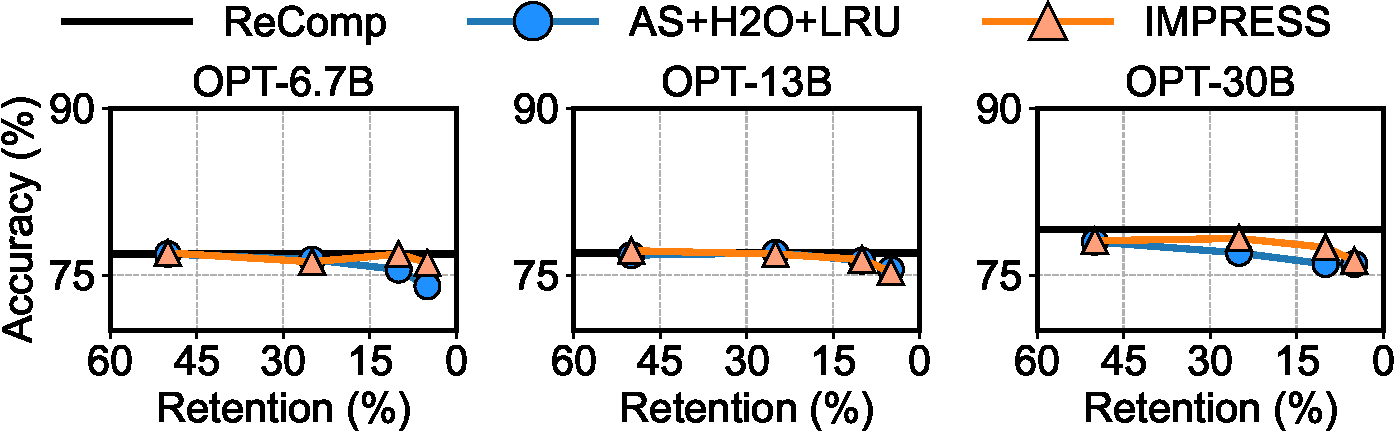
\includegraphics[width=3.3in, height=1.1in]{overall_acc1_piqa.pdf}
	}
	\hspace{0.1in}
	\subfigure[RTE]{
		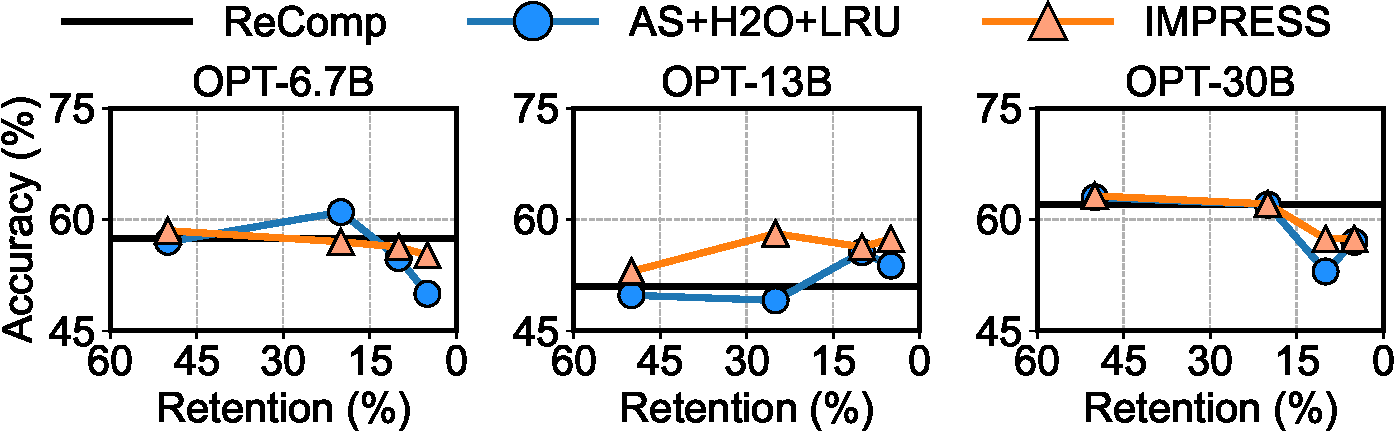
\includegraphics[width=3.3in, height=1.1in]{overall_acc1_rte.pdf}
	}
	\subfigure[COPA]{
		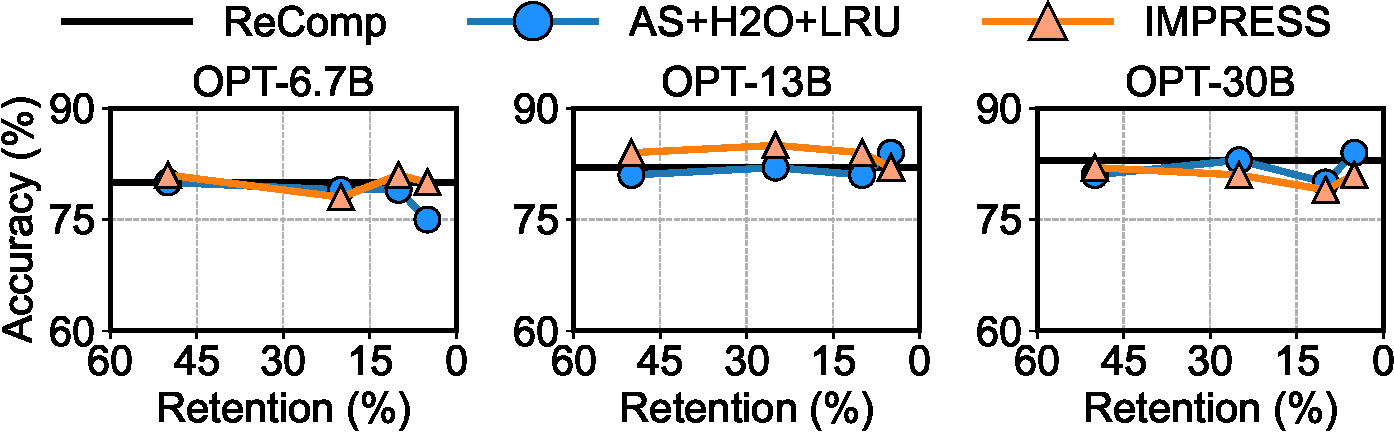
\includegraphics[width=3.3in, height=1.1in]{overall_acc1_copa.pdf}
	}
	\hspace{0.2in}
	\subfigure[OpenBookQA]{
		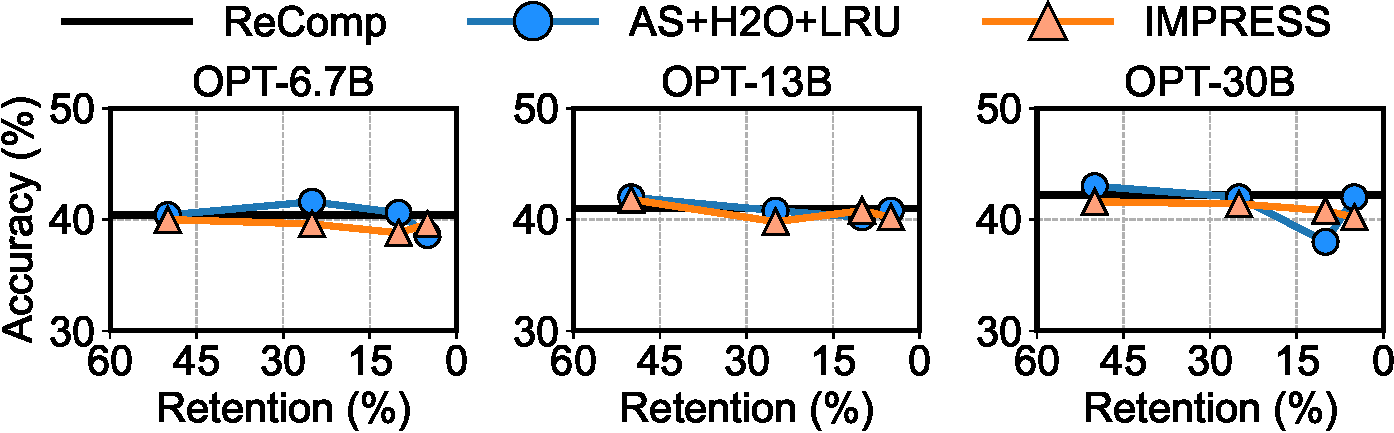
\includegraphics[width=3.3in, height=1.1in]{overall_acc1_openbookqa.pdf}
	}
	
	\vspace{-0.1in}
	\caption{
		Model generation quality of various systems across four datasets and three models.}
	\label{fig:overall_acc}
	\vspace{-0.1in}
\end{figure*}

%\noindent \textbf{Dual-cache replacement algorithm.} 
%The \pname{} system includes both GPU and CPU caches, each managed by different cache eviction strategies due to the varying granularity of data transfers from disk and CPU. Specifically, to optimize disk I/O efficiency, data is transferred from disk to CPU cache in chunks, regardless of the ratio of important KVs within each chunk. Consequently, the CPU cache eviction is only based on chunk access frequency to minimize the number of chunks loaded from the disk. 
%In contrast, when transferring data from the CPU cache to the GPU cache, only important KVs are transmitted to reduce  \ysl{the pressure on the PCIe bus}~\cite{flexgen-icml23}. Therefore, the \techbb{} method is employed in GPU cache eviction to minimize the transmission of important KVs.
%
%To achieve this, 
%we maintain two separate min-heaps in the GPU and CPU caches to assist with cache eviction. The top elements in the GPU heap are chunks with the lowest scores, while in the CPU heap, they are chunks with the lowest access frequency.
%When a new request arrives, the system first checks the radix tree-based meta data to identify reusable stored prefix KV chunks and locate whether they are located in the GPU cache, CPU cache, or disk.
%If the target chunk is in the GPU cache, after the chunk is accessed and its score is updated, it remains in the GPU cache.
%If the target chunk is in the CPU cache, its score is updated and compared with the smallest score in the GPU cache. If the target chunk's score is higher, it is swapped with the lowest-score chunk in the GPU cache; otherwise, it stays in the CPU cache.
%If the target chunk is on the disk, its access frequency is updated and compared with the lowest access frequency in the CPU cache. If the target chunk has a higher access frequency, it replaces the least-accessed chunk in the CPU; otherwise, it stays in the disk.

\noindent \textbf{Dual-cache replacement algorithm.}
% We use \techbb{} to manage both GPU and CPU caches. To achieve this, we maintain two min-heaps in CPU memory for the chunks in GPU and CPU memory to assist with cache eviction. 
% The top elements in two heaps point to the chunks with the lowest scores in the GPU and CPU caches respectively. 
% %We ensure that chunks in the GPU and CPU caches are non-redundant to maximize the amount of cached data. Additionally, 
% We ensure that all chunks' replicas are kept on disk to avoid I/O latency when evicting chunks from the CPU to disk.
We employ score-based cache replacement policy to oversee GPU and CPU caches, utilizing two min-heaps in CPU memory to manage chunks in both caches and facilitate eviction. The heaps' tops indicate the lowest-scored chunks in the GPU and CPU caches, respectively. To optimize data caching, we ensure non-redundancy between the GPU and CPU caches. Additionally, we maintain all chunk replicas on disk, thus eliminating I/O latency when chunks are evicted from CPU to disk.

Upon receiving a new request, \pname{} first identifies reusable important tokens and locates their associated chunks. If the chunk is already in the GPU cache, \pname{} utilizes the key or value vectors for inference and updates the chunk's score, retaining it in the GPU cache. If the chunk is in the CPU cache, after transferring the vectors to the GPU, \pname{} updates and compares the chunk's score with the GPU cache's lowest. If superior, it replaces the lowest-scored chunk in the GPU cache; otherwise, it stays in the CPU cache.
Should the chunk reside on disk, \pname{} loads it into CPU cache, transfers the necessary vectors to the GPU, and updates the chunk's score. This new score is then assessed against the lowest scores in both caches to decide whether the chunk should be promoted to the GPU cache, remain in the CPU cache, or stay on disk.



%\subsubsection{\techBb{}}
%当要读取的重要token的key or value vector在disk上时,\pname{} 首先会从disk加载其所在的chunk到CPU中,然后读取仅传送重要的key or value vectors 到GPU中从而减小PCIe传输量,最后决定该chunk是否被GPU或CPU缓存以备后续使用。
%However, we observed that the number of important key or value vectors in a chunk does not correlate with the chunk’s access frequency, as shown in Figure~\ref{fig:imp_token_num}. Therefore, existing systems that determine whether to cache a chunk in GPU memory or CPU memory based solely on access recency or frequency may reduce the hit ratio of important key-value pairs in the GPU cache, leading to an increase in data transferred via PCIe.
%
%To address this, we propose an importance-informed \techbb{} that further improves the GPU cache hit ratio and reduce the data transfer volume from CPU to GPU.
%The core idea is to assign a score to each chunk and use the score to determine whether it should be cached. 
%This score is defined as the cumulative number of important vectors accessed within each chunk.
%as its access frequency multiplied by the ratio of important keys or values it contains. 
%The chunks with higher scores are prioritized for caching in GPU memory, while those with lower scores are placed in CPU memory. 
%The score is updated after each chunk access.
% The ratio of important keys or values is computed as the moving average between two consecutive accesses and updated online after each chunk access.
%
%假设有三个chunk的访问频率分别是8, 10, 7;其中重要的token的数量分别是3, 1, 2。假设GPU和CPU都只能存储1个chunk,新的一些请求分别要访问8、10、7次三个chunk以获取其中重要的token用于推理。
%传统方法使用LFU缓存时会根据chunk访问频率从高到底放置如图x。那么传统方法一共需要经过PCIe传输8*3 + 7*2 = 38个vector。
%使用\techbb{}后,由于chunk1的score大于chunk2的score,因此放置如图x;那么一共需要经过PCIe传输10*1 + 7*2 = 24个vector。



\section{Implementation}
\label{impl}
%We implemented \pname{} based on the modern offloading-based LLM inference framework, FlexGen~\cite{flexgen-icml23}.
%(为什么选择这个框架?重用它的 xxx 模块)
%我们识别出探测头中重要KVusing mha 函数产生的 attention weights矩阵基于 H2O 方法 。然后基于 4.3 的方法决定加载剩下头中预测的重要 KV 还是全部KV。
%For KV reordering,  我们实现 xxx;To implement dual score-based cache management, 我们实现 xxx
\fv{
%We implemented \pname{} on top of FlexGen~\cite{flexgen-icml23}, a modern offloading-based LLM inference framework.
%We chose it because it provides a white-box implementation of models, which facilitates the integration of our I/O-efficient KV identification method. 
%Specifically, we modified the \textit{mha} function to support prefix reuse and accumulated the values in each column of the \textit{attn\_weight} matrices to evaluate the importance of each KV pair.
%We implement \pname{} on top of FlexGen~\cite{flexgen-icml23}, chosen for its white-box model implementation that aids integrating our I/O-efficient KV identification method.
We chose to implement \pname{} on top of FlexGen~\cite{flexgen-icml23} because its white-box model implementation facilitates the development of our I/O-efficient KV identification method.
 Specifically, we modified the \textit{mha} function for prefix reuse and used values in \textit{attn\_weight} to assess KV importance.
For KV reordering, we implemented the \textit{PrefixKVLayer} class to store reordered KVs and mapping lists per layer. 
For cache management, we developed the \textit{TokenCache} class with our score-based policy.
}
\section{Evaluation}
\label{eval}

\subsection{Experimental Setup}
\label{exp:setup}

\textbf{Models and system configuration.}
We conduct tests using three open-source OPT models of different scales (i.e., OPT-6.7B, OPT-13B, and OPT-30B). Our experiments are performed on a server with 2 $\times$ AMD EPYC 7763 CPUs (64 cores), 128 GB DRAM, one NVIDIA A100 GPU with 80GB HBM, and one 2TB Intel SSD whose measured read throughput is around 5GB/s. The GPU and CPU are connected via PCIe 4.0 $\times$ 16.

\noindent \textbf{Datasets and metrics.}
%We use four representative datasets covering three typical tasks involving shared prefixes: 
%(1) Few-shot tasks. We use two datasets from the lm-evaluation-harness benchmark~\cite{lmeval}: PIQA and OpenBookQA. Each request starts with two to ten examples as the few-shot prefix.
%(2) RAG-based question answering tasks. We use a reading comprehension dataset, SQuAD~\cite{squad-arxiv18}, where multiple queries are involved for the same passage prefix.
%(3) System-prompt-based tasks. Forty-five system prompts that explicitly define the functionalities of the GPT store plugins~\cite{gptsysprompt} are used as prefixes. Similar to~\cite{cacheblend-arxiv24}, we use the GPT-4 API to generate three more similar queries for each system prompt.
We select four representative datasets from the standard LM-Evaluation-Harness benchmark~\cite{lmeval}: PIQA, RTE, COPA, and OpenBookQA. 
\fv{
These datasets are designed for few-shot tasks and structured as multiple-choice questions to evaluate the capabilities of large models in commonsense reasoning, logical inference, causal reasoning, and science question answering, respectively. 
%In total, there are approximately 400 user requests for PIQA and around 1,000 requests for each of the other three datasets.
}
Due to the lack of open-source, real-world datasets for prefix reuse, we adopt a similar approach to previous work~\cite{infinigen-osdi24} by prepending two to ten few-shot examples as system prompts before each query. These system prompts are shared across different queries, with reuse frequency following a normal distribution.

%We measure model generation quality using accuracy, following the same metric employed in prior works~\cite{infinigen-osdi24, h2o-nips23}.
%We vary the user-defined prefix KV retention ratios from 50\% to 5\% to observe changes in model accuracy.
\fvc{
We measure model generation quality using accuracy, as in prior works~\cite{infinigen-osdi24, h2o-nips23}, and vary the prefix KV retention ratios from 50\% to 5\% to observe accuracy changes.
}
Additionally, to test TTFT with long prefixes as in~\cite{cachegen-sigcomm24} and to prevent runtime out-of-memory errors, we extend the prefixes to a maximum length of 4K for OPT-30B and 10K for the other OPT models.
\fv{
The average number of tokens in the request prefixes across the four datasets ranges from 4.8k to 5.7k.
}

\noindent \textbf{Baseline systems.}
We compare \pname{} with four baselines.
(1) \textit{ReComp}~\cite{alluneed-nips17}: It recomputes all prefix KVs for each request without storing or reusing them.
(2) \textit{AS-like}~\cite{attentionstore-atc24}: AttentionStore (AS)
asynchronously stores and loads all shared prefix KVs. Since it is not
open-source, we reimplement it to the best of our ability based on the paper. To
ensure a fair comparison, we additionally add the GPU cache with LRU for prefix KV
storage. Besides, we disable its scheduler-aware optimizations to make it more
suitable for general scenarios, such as preemptive scheduling environments.
(3) \textit{AS+H2O+LRU}: We combine AS-like with one of the state-of-the-art important KV selection systems, H2O~\cite{h2o-nips23}. Different from the AS-like, it asynchronously loads only important values rather than the full values of shared prefixes.
(4) \textit{AS+H2O+LFU}: It is similar to (3), but it uses LFU to manage the cache.
%We believe both (3) and (4) represent state-of-the-art systems for accelerating prefix KV loading from storage, combining existing optimization techniques.
In contrast, \pname{} selectively loads partial keys and values, 
%enables KV reordering, and employs a score-based cache management strategy.
\fvc{
reorders KVs, and uses a score-based cache management strategy.
}

% \he{By default, we allocate 10GB of GPU cache and 32GB of CPU cache to avoid runtime out-of-memory errors for all the systems.}
% The average prefix KV storage requirements for PIQA, RTE, COPA, and OpenBookQA across three models are 55 GB, 57 GB, 64 GB, and 65 GB, respectively.
% Each chunk contains 64 tokens' keys or values in all systems~\cite{chunkattention-arxiv24}.
% We clarify that in our scenario, the entire query is always retained, unlike
% existing KV pruning systems~\cite{h2o-nips23, infinigen-osdi24}.

To prevent runtime out-of-memory errors and ensure only a portion of the prefix
KVs are cached (the other KVs reside on SSD), we allocate 10GB of GPU cache and 32GB of CPU cache for prefix
KVs, leaving the remaining GPU and CPU memory for storing model weights, the KV cache
used during the decoding phase, and the input data.
%\he{By default, we assign 10GB to GPU cache and 32GB to CPU cache across all systems to prevent memory overflow.} 
On average, PIQA, RTE, COPA, and OpenBookQA require 55GB, 57GB, 64GB, and 65GB of storage for prefix KVs across three models, respectively. Uniformly, each chunk holds keys or values from 64 tokens~\cite{chunkattention-arxiv24}. 
%Note that, unlike conventional KV pruning systems~\cite{h2o-nips23, infinigen-osdi24}, we retain the full query in our scenario.

\begin{figure*}
	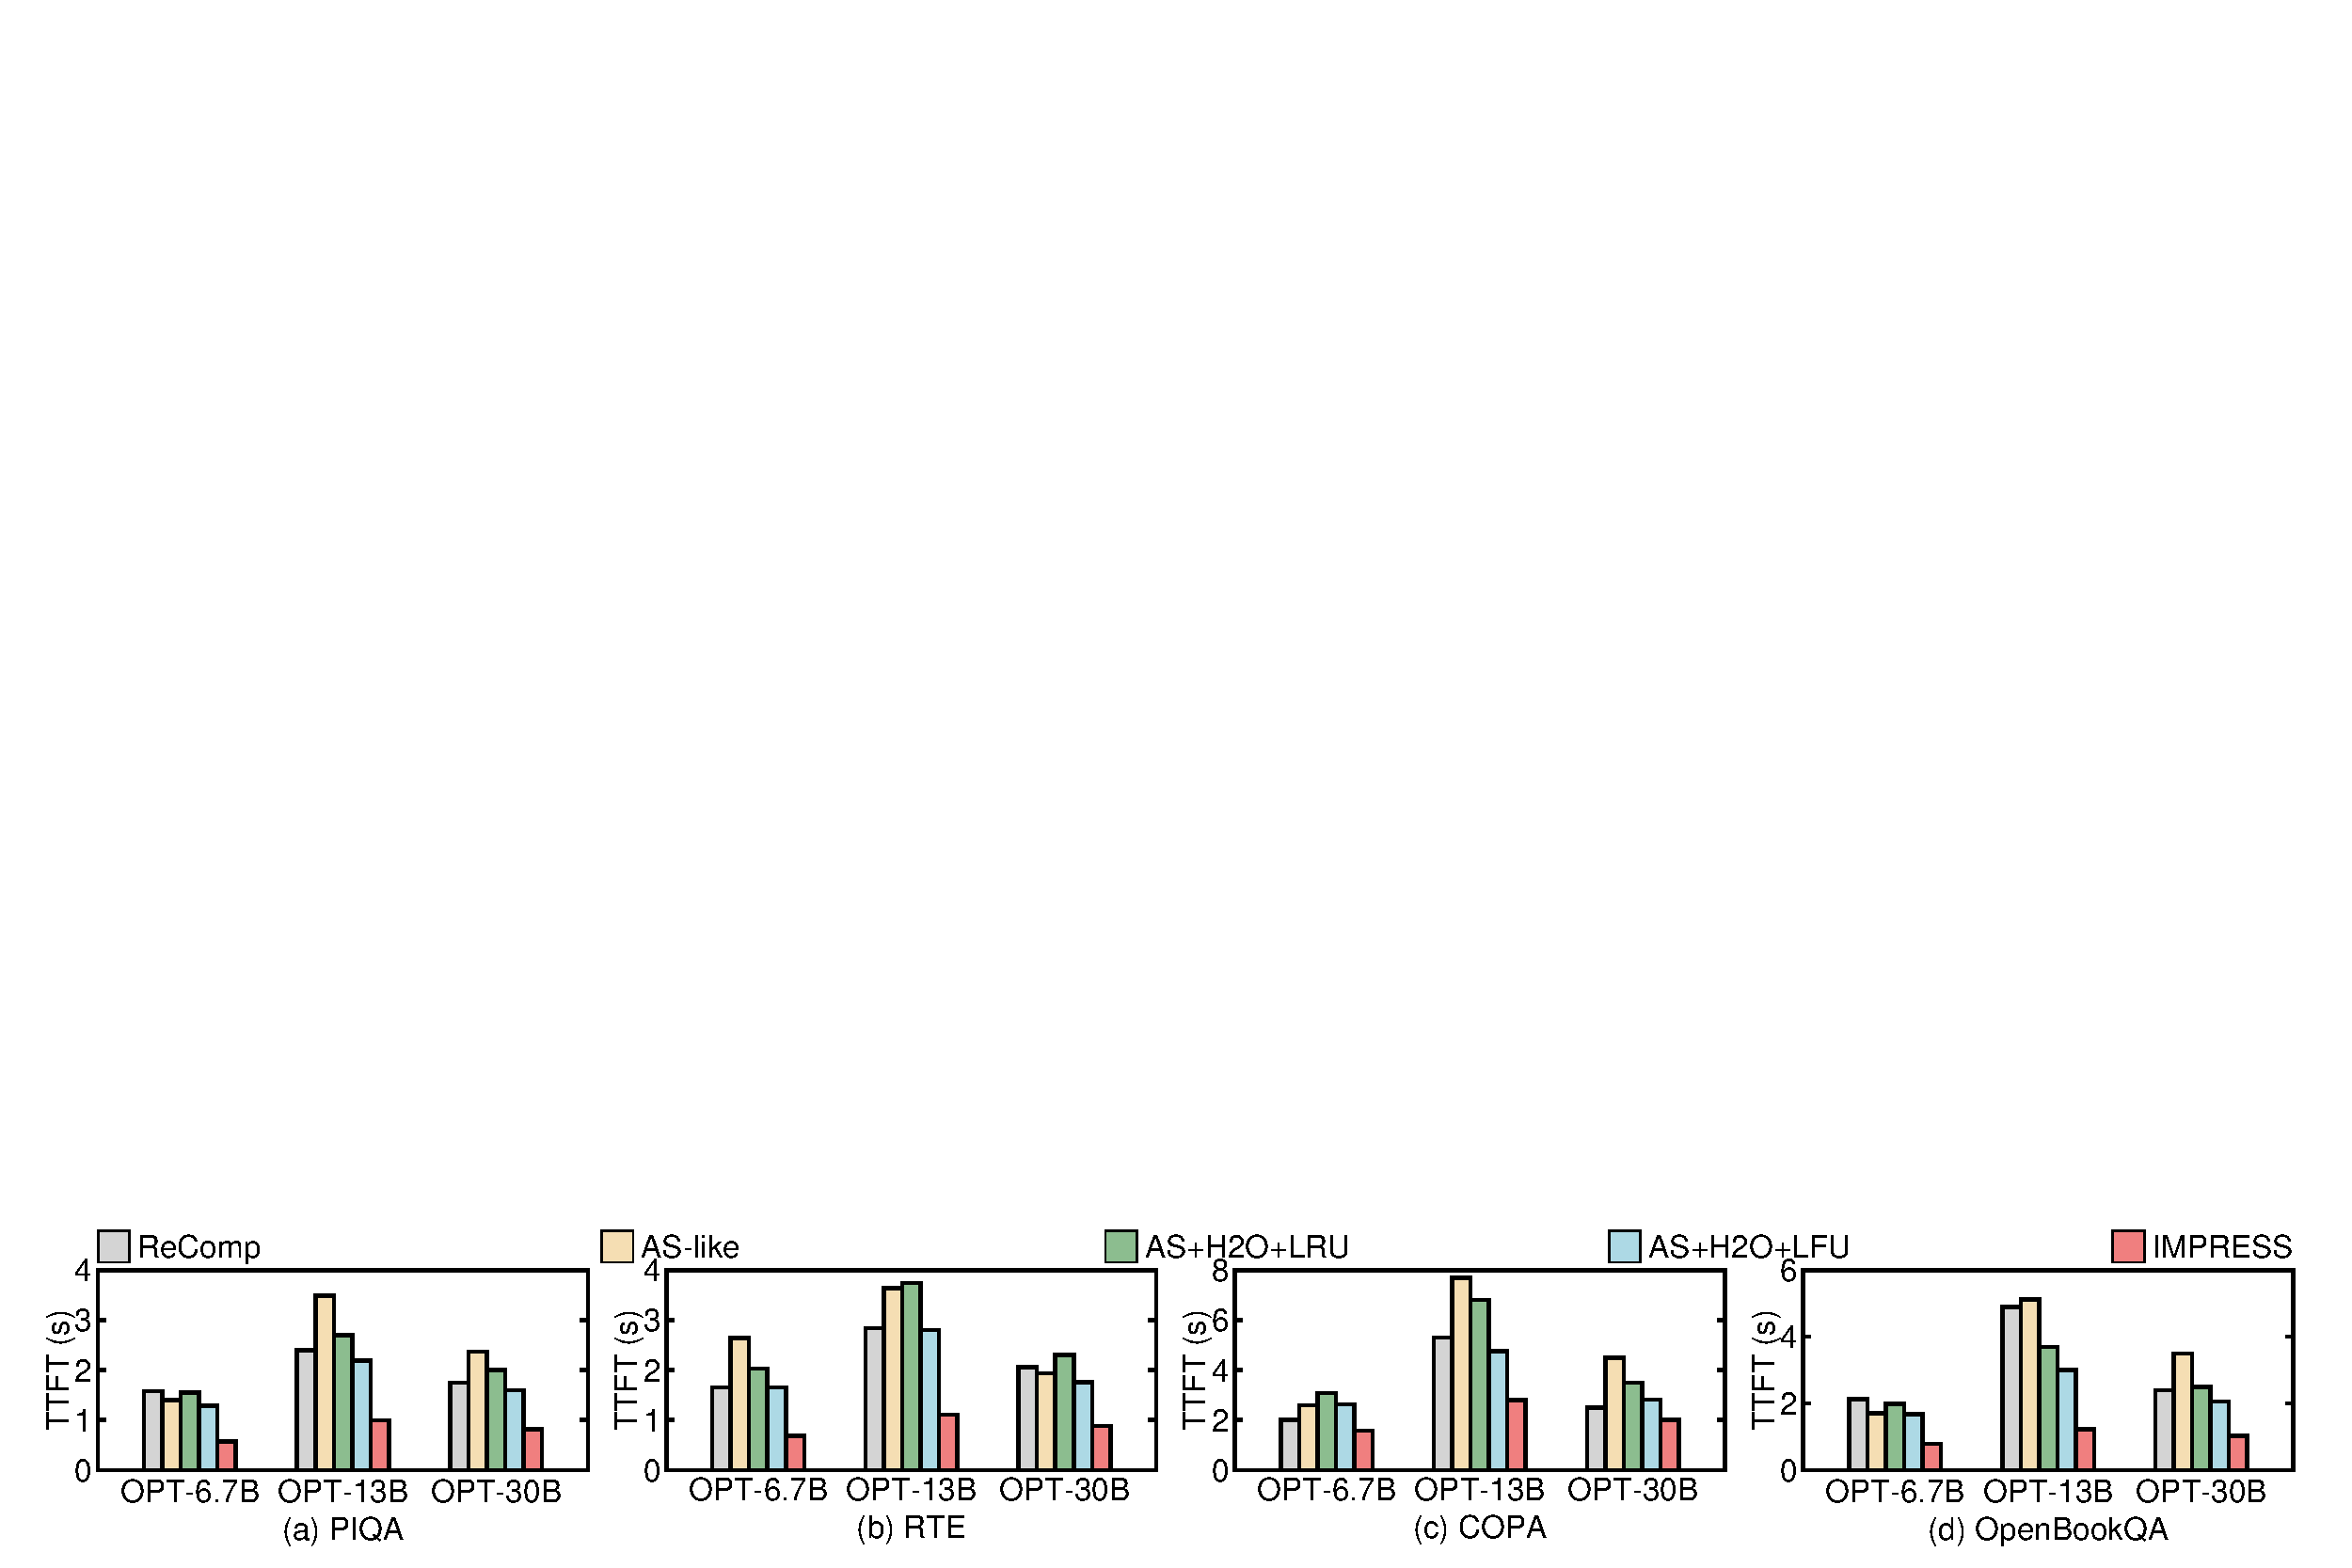
\includegraphics[width=7in, height=1in]{ttft_ds1_ds2_ds3_ds4.pdf}
	\vspace{-0.2in}
	\caption{
		The average TTFT with various systems across four dataset and three models.}
	\label{fig:overall_ttft}
	\vspace{-0.1in}
\end{figure*}

%\begin{figure*}
%	\subfigure[ds1]{
%		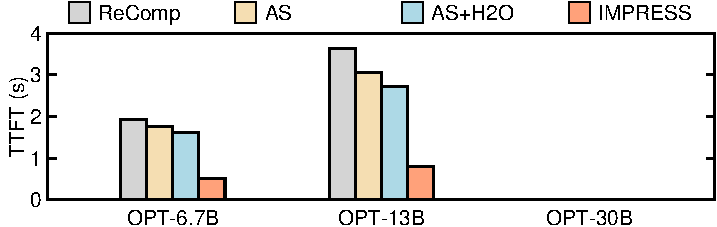
\includegraphics[width=3.3in, height=1in]{ttft_ds1.pdf}
%	}
%	\hspace{0.1in}
%	\subfigure[ds2]{
%		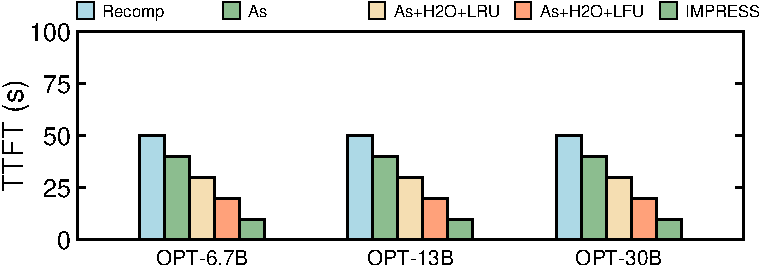
\includegraphics[width=3.3in, height=1in]{ttft_ds2.pdf}
%	}
%	\subfigure[ds3]{
%		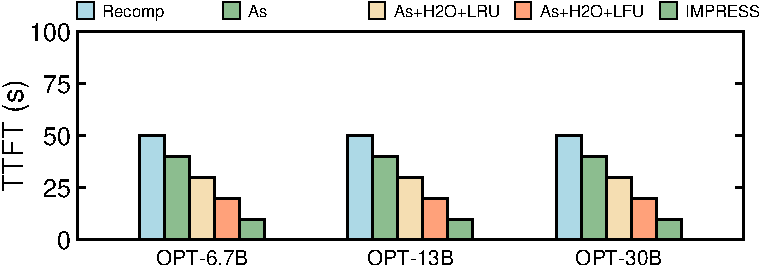
\includegraphics[width=3.3in, height=1in]{ttft_ds3.pdf}
%	}
%	\hspace{0.1in}
%	\subfigure[ds4]{
%		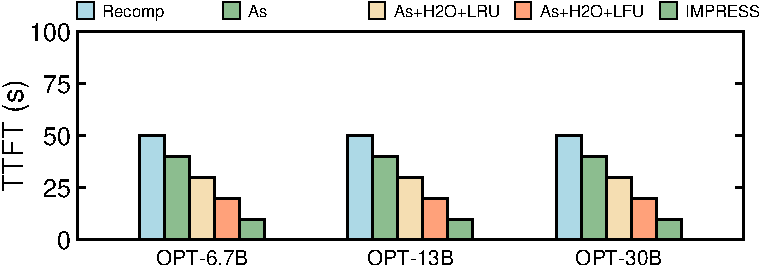
\includegraphics[width=3.3in, height=1in]{ttft_ds4.pdf}
%	}
%	\vspace{-0.1in}
%	\caption{
%		The average TTFT of various systems across four dataset and three models.}
%	\label{fig:overall_ttft}
%\end{figure*}

%\begin{figure*}
%	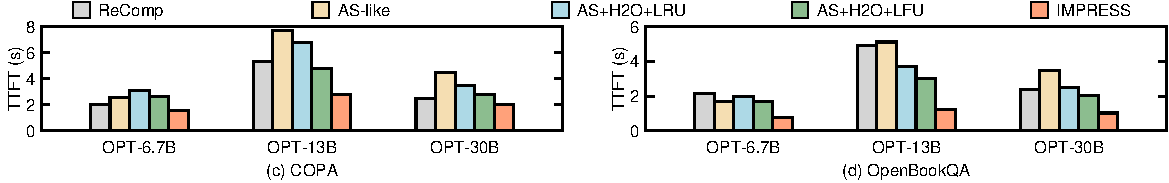
\includegraphics[width=3.4in, height=1.2in]{ttft_ds3_ds4.pdf}
%%	\vskip 1em
%	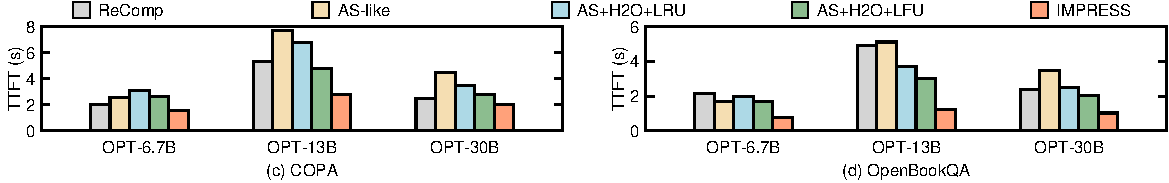
\includegraphics[width=3.4in, height=1.2in]{ttft_ds3_ds4.pdf}
%	\vspace{-0.1in}
%	\caption{
%		The average TTFT of various systems across four dataset and three models.}
%	\label{fig:overall_ttft}
%\end{figure*}


%\begin{figure*}
%	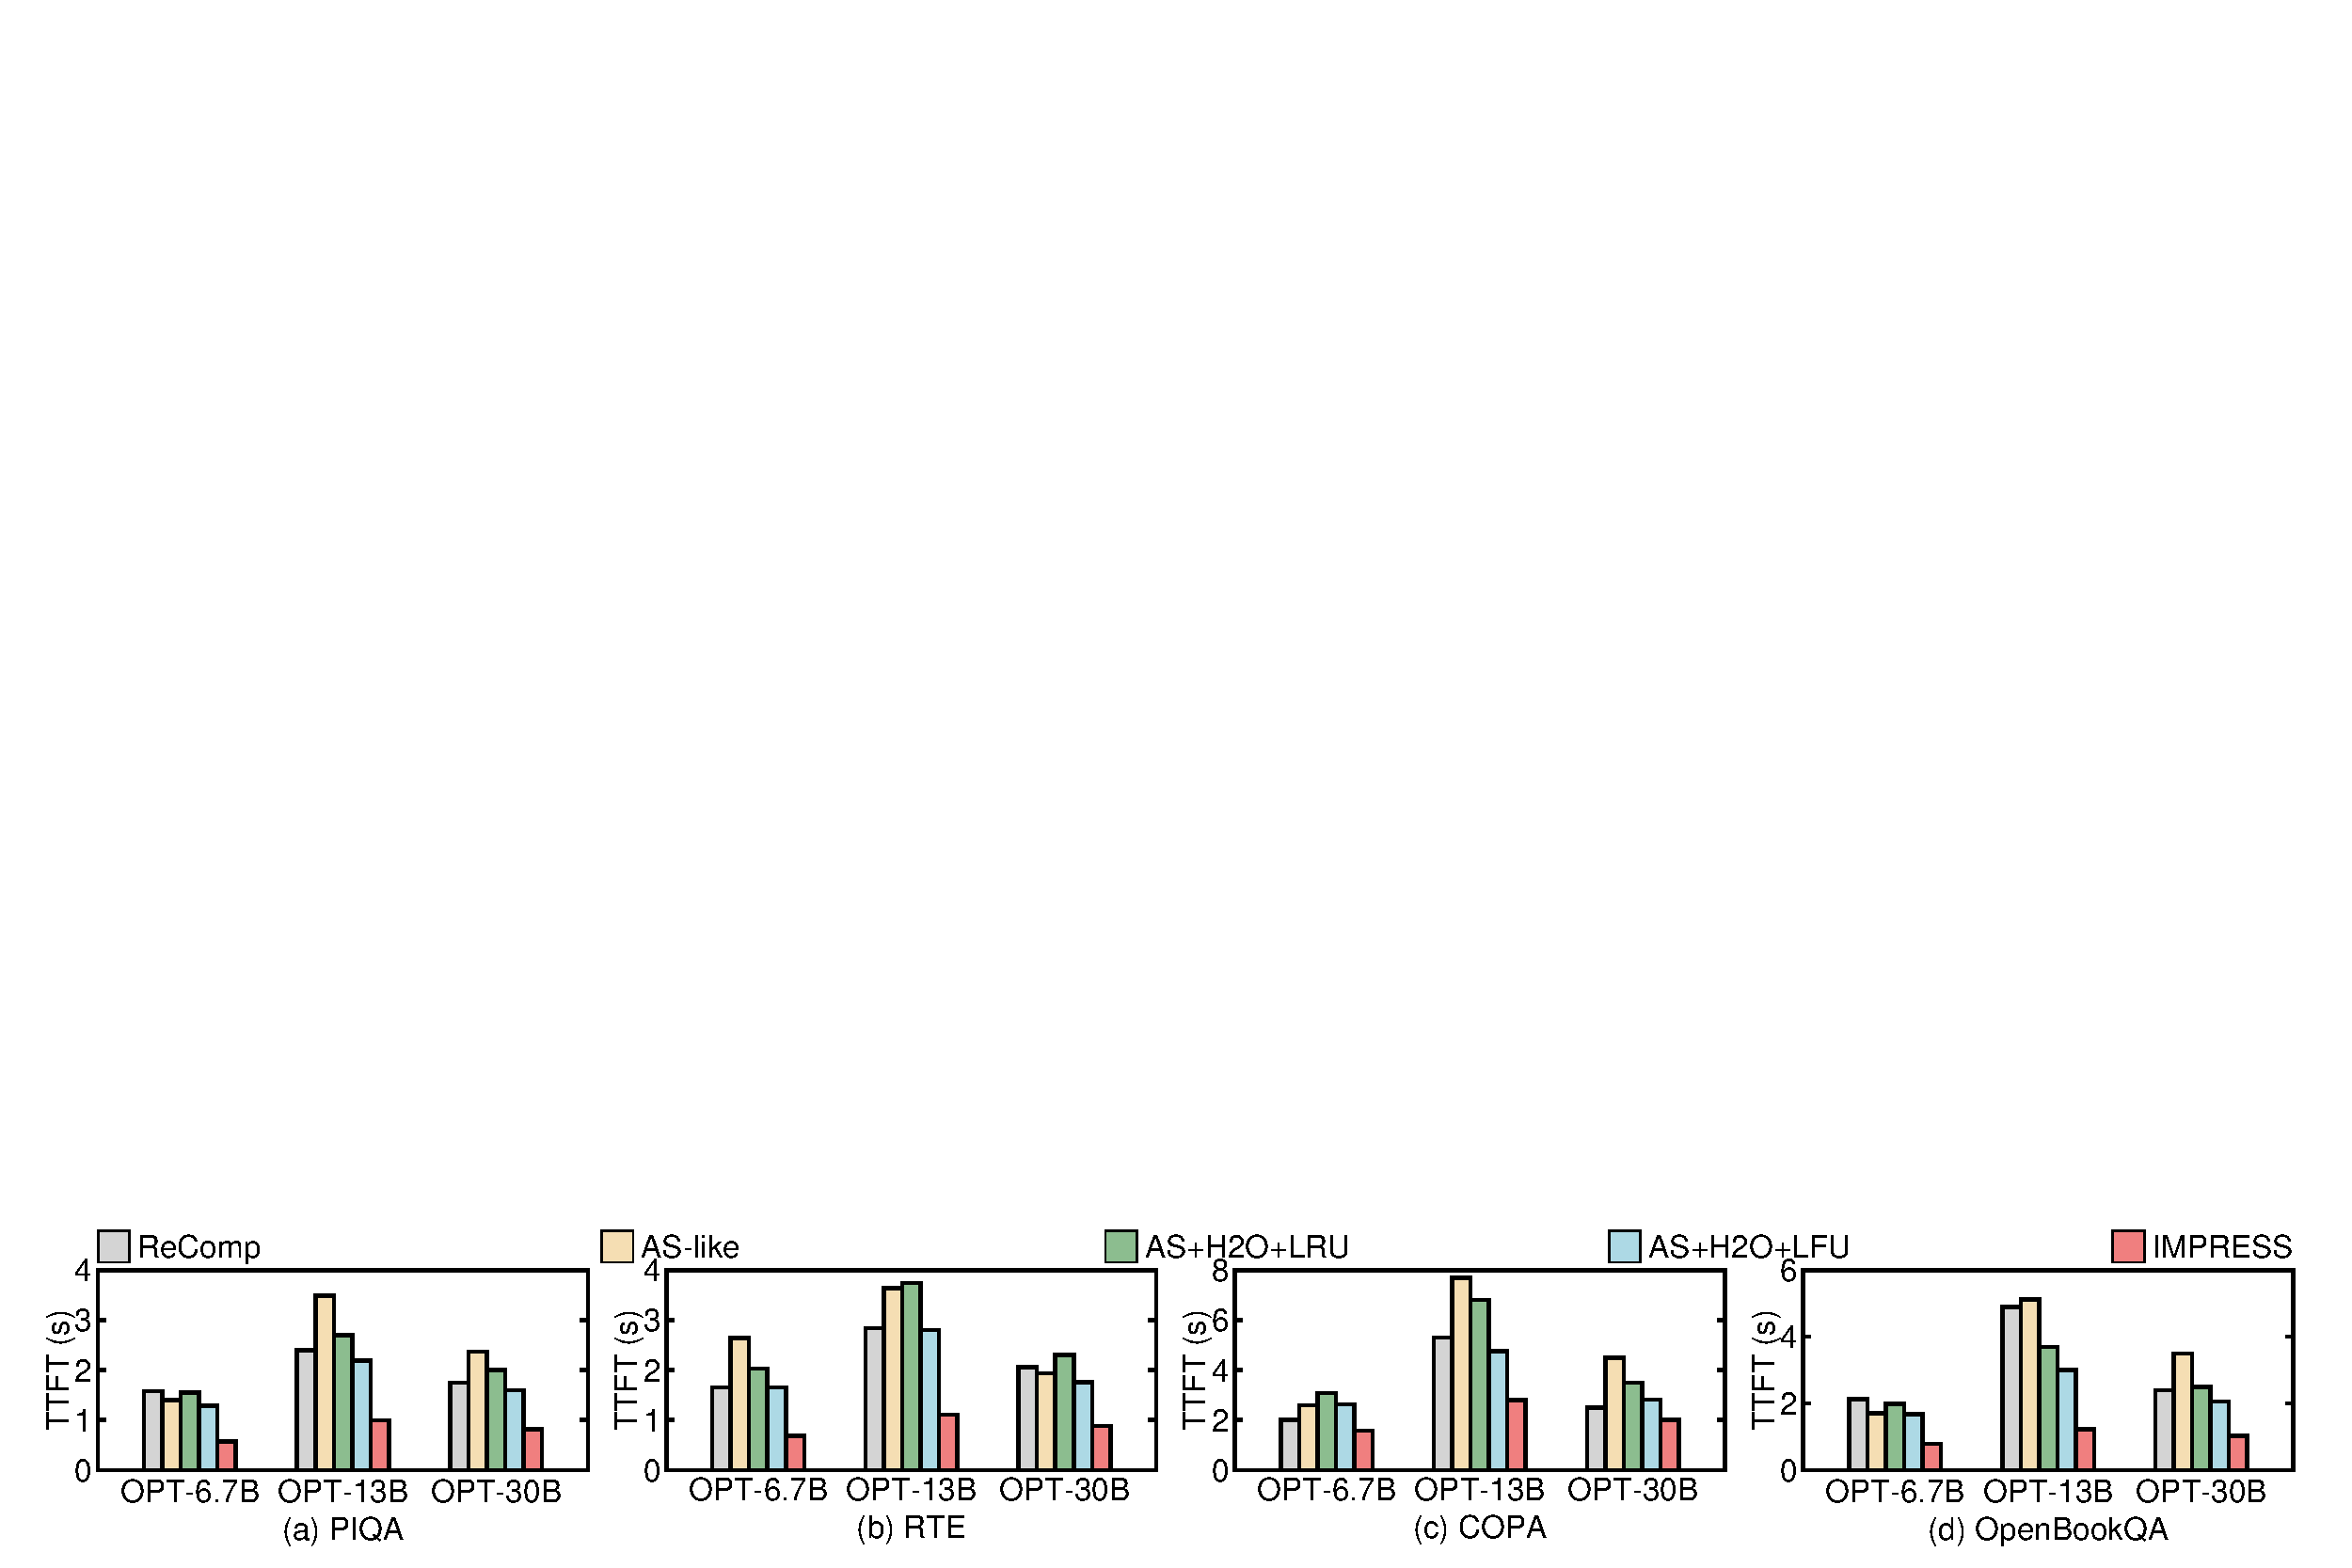
\includegraphics[width=7in, height=1.2in]{ttft_ds1_ds2_ds3_ds4.pdf}
%	\vspace{-0.1in}
%	\caption{
%		The average TTFT of various systems across four dataset and three models.}
%	\label{fig:overall_ttft}
%\end{figure*}

\begin{figure}
	\centering
	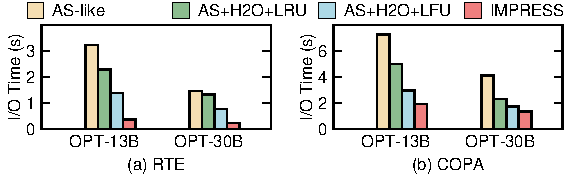
\includegraphics[width=3.3in, height=1in]{iotime.pdf}
	 \vspace{-0.1in}
	\caption{Prefix KV loading time on the RTE dataset.}
	\label{fig:iotime}
	\vspace{-0.1in}
\end{figure}



\subsection{Overall Performance}
\label{exp:overall}

\noindent \textbf{Model generation quality.}
Figure~\ref{fig:overall_acc} illustrates the impact of different systems on model generation quality at various prefix KV retention ratios. 
As ReComp and AS-like share the same accuracy, and AS+H2O+LRU and AS+H2O+LFU also show identical accuracy, we present only the accuracy of ReComp, AS+H2O+LRU, and \pname{} for simplicity.
It shows that \pname{} has a negligible impact on accuracy across these datasets
and models, achieving accuracy drop less than 1\% compared to ReComp or AS+H2O+LRU. In
some cases, \pname{} even slightly improves accuracy over ReComp, suggesting
that focusing on more important tokens can sometimes enhance generation quality.



\noindent \textbf{The average TTFT.}
%We warm up both CPU and GPU caches for all systems, \he{except ReComp}, before evaluating TTFT.
We pre-warm both CPU and GPU caches for all systems, except ReComp (which doesn’t require prefix KV reuse), before evaluating TTFT.
We set the KV retention ratio to 50\% for COPA and 25\% for the other three
datasets across all systems. With this setup, \pname{} shows an average accuracy
reduction of 0.2\% compared to ReComp.
%Figure~\ref{fig:overall_ttft} presents the average TTFT per request with different systems. 
%We have two observations.
%First, \pname{} significantly outperforms alternative systems, with a performance improvement of 1.2$\times$ to 2.8$\times$ over the leading solutions. This advantage stems from \pname{}'s ability to cut the I/O time for loading prefix KVs into GPU memory by 1.5$\times$ to 3.8$\times$, as illustrated in Figure~\ref{fig:iotime}. Conversely, other systems suffer from longer I/O times, occasionally leading to a TTFT that surpasses even ReComp's.
%Second, the performance gains of \pname{} fluctuate across different datasets and models. This variation is attributed to the distinct sizes of prefix KV data and the computational demands of each dataset and model. It's important to note that OPT-30B achieves a shorter TTFT than OPT-13B, as it handles shorter prefixes to prevent GPU memory overflow, which can cause out-of-memory errors.
\fvc{
Figure~\ref{fig:overall_ttft} shows the average TTFT per request for different systems. \pname{} outperforms alternatives, with a 1.2$\times$ to 2.8$\times$ improvement over leading solutions, due to a 1.5$\times$ to 3.8$\times$ reduction in I/O time for loading prefix KVs into GPU memory (Figure~\ref{fig:iotime}). Other systems have longer I/O times, sometimes exceeding ReComp's TTFT. Besides, \pname{}'s performance gains vary across datasets and models due to different prefix KV sizes and computational demands. Notably, OPT-30B has a shorter TTFT than OPT-13B, as it uses shorter prefixes to avoid GPU memory overflow.
}


\noindent 
\fv{
\textbf{The tail latency.} \pname{} achieves the shortest p99 tail TTFT. For example, on the RTE dataset with OPT-30B model, the p99 latencies for ReComp, AS-like, AS+H2O+LRU, AS+H2O+LFU, and \pname{} are 3.9s, 9.3s, 6.6s, 5.9s, and 2.95s, respectively. This shows \pname{} effectively reduces the tail I/O latency when KVs are loaded from SSD.
}

\begin{figure}
	\centering
	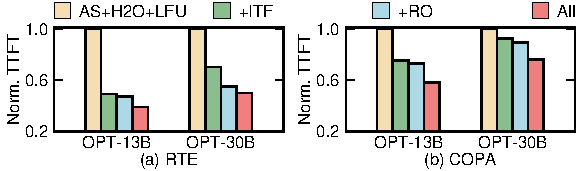
\includegraphics[width=3.3in, height=1in]{indiv_ds1_ds2.pdf}
	\vspace{-0.1in}
	\caption{The performance impact of each optimization.}
	\label{fig:indiv}
	\vspace{-0.1in}
\end{figure}

\subsection{Impact of Individual Techniques}
\label{exp:indiv}

%\begin{figure}
%	\centering
%	\subfigure[RTE]{
%		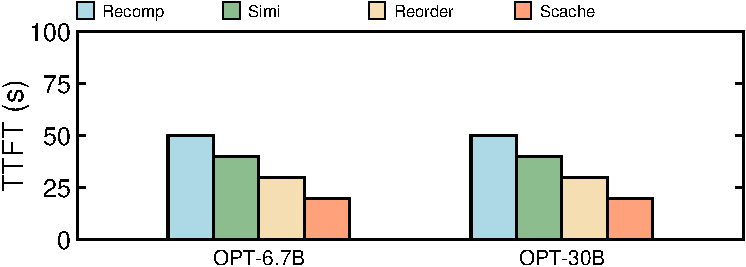
\includegraphics[width=1.5in, height=1in]{indiv_ds1.pdf}
%		\label{fig:indiv_ds1}
%	}
%	\hspace{0.06in}
%	\subfigure[COPA]{
%		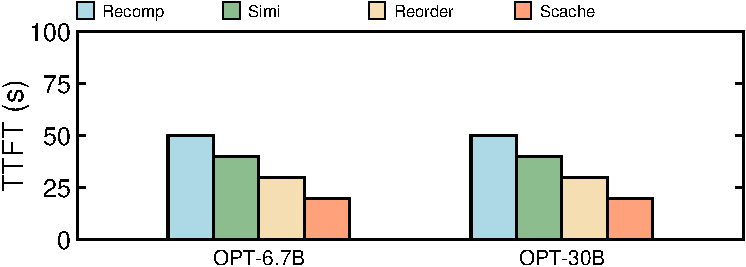
\includegraphics[width=1.5in, height=1in]{indiv_ds2.pdf}
%		\label{fig:indiv_ds2}
%	}
%	\vspace{-0.2in}
%	\caption{
%		The performance impact of each optimizatio.}
%	\label{fig:indiv}
%\end{figure}

%Figure~\ref{fig:indiv} illustrates the impact of each optimization in \pname{}.
%We use the current SOTA system \textit{AS+H2O+LFU} as the baseline and normalize
%its TTFT to one. \textit{+ITF} represents the version which enhances baseline
%with \techa{}, which only loads important KVs; \textit{+RO} builds upon
%\textit{+ITF} by enabling the \techba{} technique; \textit{All} refers to the
%version that further incorporates the \techbb{} strategy on top of
%\textit{+RO}. 
\fvc{
Figure~\ref{fig:indiv} shows the impact of each optimization. Using the current SOTA system \textit{AS+H2O+LFU} as the baseline (TTFT normalized to one), \textit{+ITF} adds \techa{} for loading important KVs, \textit{+RO} enables \techba{} on \textit{+ITF}, and \textit{All} incorporates \techbb{} on \textit{+RO}.
}
%Due to space limitations, we only present the results of
%two models and two datasets.
%From the figure, we have two findings. First, we observe that each optimization further reduces TTFT, with \textit{All}
%achieving the shortest TTFT. This demonstrates the effectiveness of each
%individual technique in \pname{}. 
%Second, the contributions of different techniques vary across models and datasets. For instance, in OPT-30B on the RTE dataset, the respective contributions of the three techniques are 60\%, 30\%, and 10\%. In contrast, on the COPA dataset with OPT-13B, the contributions are 36\%, 8\%, and 56\%, respectively.
\fvc{
We observe that each optimization reduces TTFT, with \textit{All} achieving the shortest TTFT, showing the effectiveness of \pname{}'s individual techniques. Besides, technique contributions vary across models and datasets. For example, in OPT-30B on RTE, the contributions of the three techniques are 60\%, 30\%, and 10\%, while on COPA with OPT-13B, they are 36\%, 8\%, and 56\%.
}


% To understand the impact of each optimization on OPT-30B,
% Figure~\ref{fig:indiv_a} shows the average ratio of KVs loaded at each layer for
% OPT-30B on
% PIQA dataset in \textit{+ITF} sytem. 
% \textit{+ITF} can dynamically decide whether to load partial or full KVs for different layers, striking a balance between model accuracy and TTFT.
% Figure~\ref{fig:indiv_b} shows that, after enabling \techba{}, the number of
% loaded chunks decreases by an average of 1.2$\times$. This is because important
% keys and values are placed in the same chunk, reducing the number of chunks that
% need to be loaded for reusing important token KVs. 
% This result indicates the effectiveness of \techba{}.
% Figure~\ref{fig:indiv_c}shows the change in GPU hit ratio after enabling the
% \techbb{} technique. It reveals that the average GPU hit ratio increases from
% 68\% to 80\% across the four datasets. This reduces PCIe data transfer, which
% explains why \textit{All} achieves the lowest TTFT.

Figure~\ref{fig:indiv_a} shows the average KV loading ratio per layer for OPT-30B on the PIQA dataset using the \textit{+ITF} system, which dynamically adjusts KV loading to optimize the trade-off between accuracy and TTFT.
Figure~\ref{fig:indiv_b} indicates that enabling \techba{} results in an average 1.2$\times$ reduction in loaded chunks, as it consolidates important keys and values into fewer chunks.
%, streamlining the loading process for important token KVs.
Figure~\ref{fig:indiv_c} shows that \techbb{} boosts the average GPU hit ratio from 68\% to 80\% across four datasets, thereby reducing PCIe data transfers.
%and contributing to the lowest TTFT in the \textit{All} configuration.


\begin{figure}
	\centering
	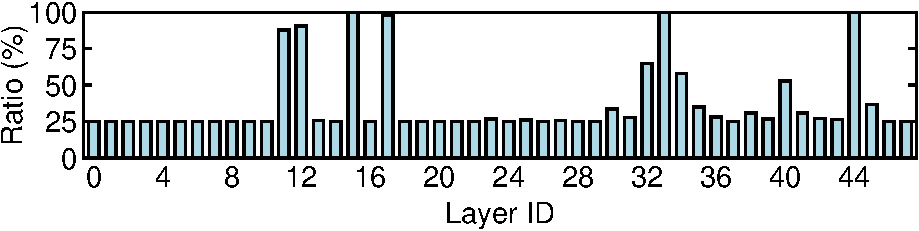
\includegraphics[width=3.3in, height=0.8in]{indiv_a_ds1.pdf}
	\vspace{-0.1in}
	\caption{The retention of KVs per model layer using \techa{}.}
	\label{fig:indiv_a}
	 \vspace{-0.1in}
\end{figure}


\begin{figure}
	\centering
	\begin{minipage}{1.6in}
		% \centering
		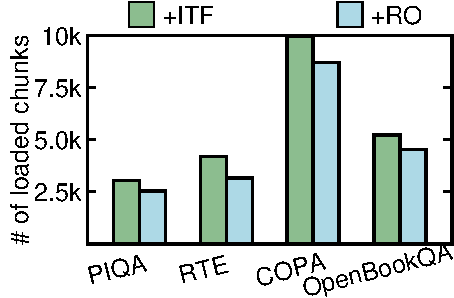
\includegraphics[width=1.6in,height=1in]{indiv_b_cknum.pdf}
		\vspace{-0.2in}
		\caption{
			The impact of \techba{} on the number of loaded chunks.
		}
		\label{fig:indiv_b}
	\end{minipage}
	\hspace{0.05in}
	\begin{minipage}{1.6in}
		\centering
		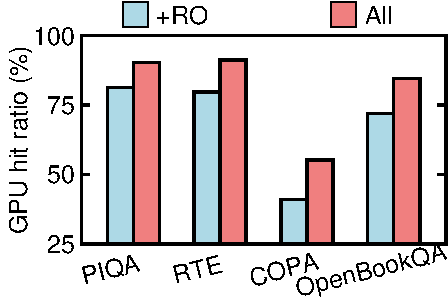
\includegraphics[width=1.6in, height=1in]{indiv_c_13b.pdf}
		\vspace{-0.2in}
		\caption{
			The impact of scored-based cache management on GPU hit ratios.
		}
		\label{fig:indiv_c}
	\end{minipage} 
	\vspace{-0.2in}
\end{figure}




%\begin{figure}
%	\centering
%	\subfigure[Number of loaded chunks]{
%		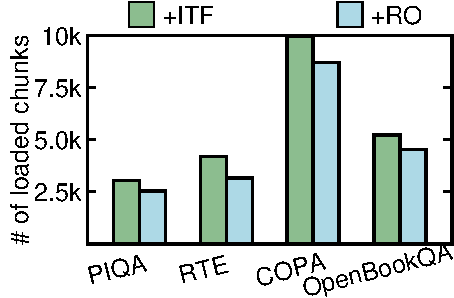
\includegraphics[width=1.5in, height=1in]{indiv_b_cknum.pdf}
%	}
%	\hspace{0.06in}
%	\subfigure[Important KV ratio]{
%		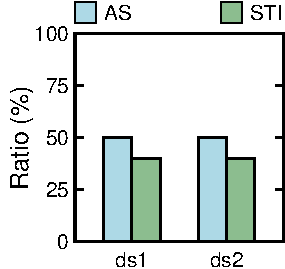
\includegraphics[width=1.5in, height=1in]{indiv_b_ckratio.pdf}
%		\label{fig:indiv_b_ratio}
%	}
%	\vspace{-0.1in}
%	\caption{
%		Comparison of the total number of loaded chunks and the average important KV ratio in each chunk before and after using \techba{}.}
%	\label{fig:indiv_b}
%\end{figure}


%\begin{figure}
%	\centering
%	\subfigure[ds1]{
%		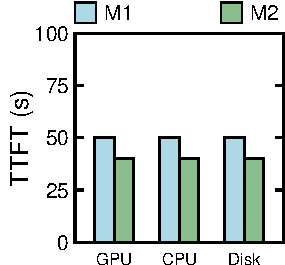
\includegraphics[width=1.5in, height=1in]{indiv_c_ds1.pdf}
%	}
%	\hspace{0.06in}
%	\subfigure[ds2]{
%		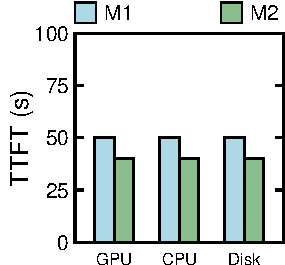
\includegraphics[width=1.5in, height=1in]{indiv_c_ds2.pdf}
%	}
%	\vspace{-0.1in}
%	\caption{
%		Comparison of the cache hit ratios.}
%	\label{fig:indiv_c}
%\end{figure}

% \input{tex/exp-reduction}
% \input{tex/exp-largedataset}
\subsection{Sensitivity Analysis}
\label{exp:sensi}


%\begin{figure}
%	
%	\centering
%	\subfigure[The impact of alpha value]{
%		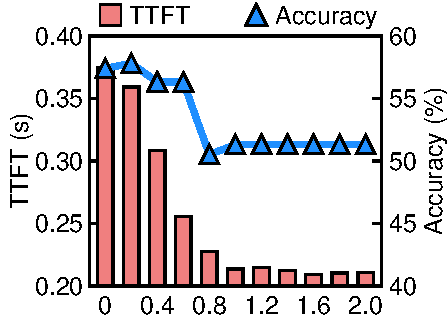
\includegraphics[width=1.5in, height=1.0in]{sensitivity.pdf}}
%	\hspace{0.06in}	
%	\subfigure[The impact of chunck size]{
%		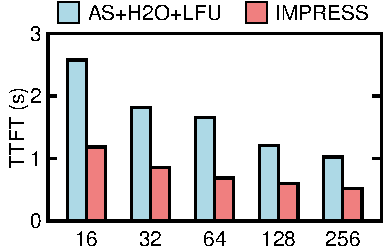
\includegraphics[width=1.5in, height=1in]{indiv_c_rte.pdf}
%	}
%	\vspace{-0.1in}
%	\caption{xxx}
%	\label{fig:sensitivity_alpha}
%\end{figure}

\noindent \textbf{Alpha value of similarity threshold.} 
% Figure~\ref{fig:sensitivity_alpha} shows the results for model inference accuracy and TTFT as the alpha value is adjusted from 0 to 2. 
% It shows that as the alpha value increases, TTFT decreases, but the model inference accuracy also drops. This is because a larger alpha value lowers the similarity threshold, making it easier for the similarity of the important token index sets in the probe heads to exceed the threshold, resulting in fewer KVs being loaded. (as discussed in \cref{sec:techa}). 
% Similar trends are observed across other datasets. 
% Therefore, we set alpha to 0.6 to achieve lower TTFT while maintaining high inference accuracy.
Figure~\ref{fig:sensitivity_alpha} depicts the impact of varying the alpha value on inference accuracy and TTFT, ranging from 0 to 2. The findings indicate that while an increased alpha reduces TTFT, it marginally affects inference accuracy due to a lowered similarity threshold, leading to less KV loading. This trend is consistent across datasets. Thus, we optimize alpha at 0.6 for a balance between low TTFT and high inference precision.

\noindent \textbf{Chunk size.} 
% Figure~\ref{fig:sens_ck} shows the TTFT results of the current state-of-the-art system and \pname{} as the chunk size is adjusted from 16 to 256. Since chunk size does not affect accuracy, we omit it from the figure. 
% We observe that across different chunk sizes, \pname{} consistently outperforms
% AS+H2O+LFU system by 2.2$\times$ to 2.4$\times$. This demonstrates the
% superiority of the \pname{} system under various chunk sizes.
Figure~\ref{fig:sens_ck} compares the TTFT of the leading system and \pname{} with chunk sizes ranging from 16 to 256. Notably, \pname{} achieves 2.2$\times$ to 2.4$\times$ improvement over the AS+H2O+LFU system across all sizes, underscoring \pname{}'s robustness regardless of chunk dimensions. Accuracy, being unaffected by chunk size, is not depicted.







\noindent 
\fv{
\textbf{Dataset size.}
%We varied the number of prefixes (i.e., few-shot examples) to create variants of the OpenBookQA with different dataset sizes from 65GB to 400GB. Figure~\ref{fig:sens_datasetsize} shows that \pname{} consistently outperforms the leading comparison systems with 
%the speedup of \pname{} varies from 1.2$\times$ to 2.0$\times$.
% increases from x$\times$ to y$\times$ as the 
% dataset grows from 65GB to 400GB compared to the leading baseline. This is because larger datasets exacerbate I/O bottlenecks, allowing \pname{} to achieve greater performance improvements.
We vary the number of prefixes (i.e., few-shot examples) to create different variants of OpenBookQA, with dataset sizes ranging from 65GB to 400GB. Figure~\ref{fig:sens_datasetsize} shows that \pname{} consistently outperforms the leading comparison system, AS+H2O+LFU, achieving speedups ranging from 1.2$\times$ to 2.0$\times$.
}

\noindent 
\fv{
\textbf{Model type.} 
Figure~\ref{fig:sens_modeltype} shows the average TTFT for Llama2-7B and Llama2-13B models on PIQA and COPA. It demonstrates that \pname{} achieves a 1.7$\times$-2.7$\times$ speedup on Llama models, attributed to similar reasons in~\cref{exp:overall}.
}


\subsection{Overhead Analysis}
\label{exp:overhead}

\begin{figure}
	\centering
	\begin{minipage}{1.6in}
		% \centering
		\includegraphics[width=1.6in,height=1in]{sensitivity.pdf}
		\caption{
			Results of various alpha values.
		}
		\label{fig:sensitivity_alpha}
	\end{minipage}
	\hspace{0.04in}
	\begin{minipage}{1.6in}
		\centering
		\includegraphics[width=1.6in, height=1in]{indiv_c_rte.pdf}
		\caption{
			Results of various chunk sizes.
		}
		\label{fig:sens_ck}
	\end{minipage} 
	\vspace{-0.15in}
\end{figure}

\noindent \textbf{Time overhead.} 
% The \techa{} technique in \pname{} loads the keys from the probe heads and calculates the important token index set. Although this process introduces some additional I/O and computation time, it accounts for 17\% on average in our system. 
% %This is because there are only three probe heads, so the required loading and computation are minimal.
% Additionally, the \techba{} technique sorts tokens by importance and repacks them to disk. The total execution time in our experiments is under one minute. Note that this process is asynchronous and does not affect TTFT, as it is not part of the critical path.
The \techa{} technique in \pname{} loads keys from the probe heads to determine the important token index set. While this adds some I/O and computation overhead, it averages only 6\% of our system's overhead due to the limited number of probe heads, resulting in minimal loading and computation.
Furthermore, \techba{} asynchronously sorts tokens by importance and repacks them onto disk, with a total experimental execution time of less than one minute. This process is non-intrusive to TTFT as it operates outside the critical path.

\noindent \textbf{Space overhead.} 
%\techba{} requires adding a mapping list to the metadata of each chunk to store the mapping between token positions before and after reordering. Furthermore, \techbb{} adds an extra score to each chunk. When the chunk size is 64, the total size of the mapping list and score accounts for less than 0.5\% of the chunk’s memory footprint.
%, which is acceptable. 
\fvc{
\techba{} adds a mapping list to each chunk's metadata for token position mappings post-reordering. Score-based cache management adds a score per chunk. With a 64-token chunk size, these additions account for less than 0.5\% of the chunk's memory. 
}
Additionally, to avoid loading data from other heads when loading keys from the probe heads, we redundantly store the keys from the probe heads separately. 
This accounts for 1.2\% of the total storage of all prefix KVs, which is a minimal cost considering high-capacity disks.
%Additionally, to shorten the keys from probe heads loading time, \pname{} redundantly stores them on disk, avoiding wasted disk I/O bandwidth from other heads in the same chunk. The disk space consumed by these redundant probe head stores is 1.2\% of the total prefix KV storage, which is a minimal cost considering the availability of cheap, high-capacity disks.




\section{Related Work}
\label{related}

\noindent \textbf{KV cache reuse.}
%Some works~\cite{alluneed-nips17, scaling-mlsys23, vllm-sosp23, flexgen-icml23} focus on reusing previously stored KV caches across different iterations within a request to reduce computation, and optimized memory allocation to support larger KV cache at runtime. These efforts target reducing decoding phase and are orthogonal to \pname{} which targets  prefill phase. Combining them with \pname{} can further accelerate the whole inference process.
%Recent studies~\cite{attentionstore-atc24, chunkattention-arxiv24, hydragen-arxiv24, ragcache-arxiv24, sglang-arxiv23, cachegen-sigcomm24} reuse shared prefix KV caches across different requests to reduce prefill latency (i.e., TTFT). However, these works load the entire prefix KVs, leading to high I/O latency when the KVs are stored on disk. In contrast, \pname{} prefetches only important prefix KVs, reducing I/O latency. 
%Other efforts~\cite{promptcache-mlsys24, cacheblend-arxiv24} explore finer-grained reuse of prefix KVs at the text segment level, which is orthogonal to \pname{} and can be combined to enable more KV reuse.
\fvc{
Some works~\cite{alluneed-nips17, scaling-mlsys23, vllm-sosp23, flexgen-icml23} accelerate the decoding phase by reusing KVs across iterations within a request. These are orthogonal to \pname{}, which targets the prefill phase.
Recent studies~\cite{attentionstore-atc24, chunkattention-arxiv24, hydragen-arxiv24, ragcache-arxiv24, sglang-arxiv23, cachegen-sigcomm24} reuse shared prefix KVs across requests to reduce prefill latency (i.e., TTFT), but load entire prefix KVs, causing high I/O latency when KVs are on disk. In contrast, \pname{} prefetches only important prefix KVs, reducing I/O latency. 
Other efforts~\cite{promptcache-mlsys24, cacheblend-arxiv24} explore finer-grained reuse of prefix KVs at the text segment level, which is orthogonal to \pname{} and can be combined to enable more KV reuse.
}


\begin{figure}
	\centering
	\begin{minipage}{1.6in}
		% \centering
		\includegraphics[width=1.6in,height=1in]{sens_datasetsize.pdf}
		\vspace{-0.1in}
		\caption{
			\fv{Results on various dataset sizes.}
		}
		\label{fig:sens_datasetsize}
	\end{minipage}
	\hspace{0.04in}
	\begin{minipage}{1.6in}
		\centering
		\includegraphics[width=1.6in, height=1in]{sens_llama.pdf}
		\vspace{-0.1in}
		\caption{
			\fv{Results on Llama (LM) models.}
		}
		\label{fig:sens_modeltype}
	\end{minipage} 
	\vspace{-0.15in}
\end{figure}

\noindent \textbf{KV pruning and quantization.}
%Recent studies~\cite{scissorhands-nips23, flexgen-icml23, h2o-nips23, infinigen-osdi24} demonstrate that LLM inference can achieve comparable output quality using only a subset of important KVs, proposing various algorithms to better predict and identify these KVs. However, they require the full keys during the prefill phase, which makes them suboptimal when directly combined with prefix KV storage systems due to the high I/O load. 
%In contrast, \pname{} leverages the similarity of important token indices across heads, allowing the identification of important KVs with minimal I/O, reducing TTFT while maintaining high accuracy.
%Other works~\cite{flexgen-icml23, cachegen-sigcomm24, kivi-arxiv24, kvquant-arxiv24, wkvquant-arxiv24} focus on quantizing KVs to reduce the bit count needed for each key and value element. These quantization techniques can be applied alongside \pname{} to further decrease data load.
\fvc{
Recent studies~\cite{scissorhands-nips23, flexgen-icml23, h2o-nips23, infinigen-osdi24} show LLM inference can achieve similar output quality using only a subset of KVs, proposing various methods to identify these KVs. 
However, they require full keys during the prefill phase, leading to high I/O latency when combined with prefix KV storage systems. 
\pname{} leverages the similarity of important token indices across heads to identify important KVs with minimal I/O, reducing TTFT while maintaining high accuracy. 
}
%Others~\cite{flexgen-icml23, cachegen-sigcomm24, kivi-arxiv24, kvquant-arxiv24, wkvquant-arxiv24} focus on quantizing KVs to reduce the bit count for each key and value element. These quantization techniques can be applied alongside \pname{} to further decrease data load.
\fvc{
Others~\cite{flexgen-icml23, cachegen-sigcomm24, kivi-arxiv24, kvquant-arxiv24, wkvquant-arxiv24} focus on KV quantization to reduce bit counts per key and value element. They can complement \pname{} to further decrease data load.
}


\noindent \textbf{Other efficient LLM serving systems.}
Some works optimize other aspects of inference systems, such as request scheduling~\cite{orca-osdi22, taming-osdi24}, model parallelism strategies~\cite{alpaserve-osdi23, loongserve-arxiv24}, prefill-decoding decoupling~\cite{distserve-osdi24, splitwise-isca24, pdserve-arxiv24, tetriinf-arxiv24, dv-arxiv24}, and distributed KV cache~\cite{infinite-arxiv24, mooncake-arxiv24}. These optimizations are also orthogonal to \pname{} and can complement its improvements.

%\section{Discussion}
\label{discus}
\section{Conclusion}
\label{conclusion}
Existing prefix KV reuse systems do not always reduce TTFT, especially when disk
I/O latency is involved in large-scale LLM services. We propose \pname{}, a
multi-tier prefix KV storage system to 
minimize I/O delay by only loading important KVs. Simply applying existing important token identification
algorithms is suboptimal, as the reduction in I/O is limited. Therefore, we
first introduce the I/O-efficient \techa{} algorithm to identify important KVs
with minimal I/O. Then, we propose \techb{} to optimize storage and caching,
further reducing TTFT. Our experiments show that \pname{} reduces TTFT by up to
2.8$\times$ compared to state-of-the-art systems, while maintaining comparable
inference accuracy.

\section*{Acknowledgments}
\fv{
We sincerely thank the anonymous reviewers for their constructive suggestions. 
This work was supported in part by the National Key Research and Development Program of China (2023YFB4502100), 
the National Science Foundation of China (62172361), 
the Major Projects of Zhejiang Province (LD24F020012), 
the Open Project Program of Wuhan National Laboratory for Optoelectronics (2023WNLOKF005),  
and the Pioneer and Leading Goose R\&D Program of Zhejiang Province (2024SSYS0002).
}


%-------------------------------------------------------------------------------
% \section*{Acknowledgments}
% %-------------------------------------------------------------------------------

% The USENIX latex style is old and very tired, which is why
% there's no \textbackslash{}acks command for you to use when
% acknowledging. Sorry.

% %-------------------------------------------------------------------------------
% \section*{Availability}
% %-------------------------------------------------------------------------------

% USENIX program committees give extra points to submissions that are
% backed by artifacts that are publicly available. If you made your code
% or data available, it's worth mentioning this fact in a dedicated
% section.

%-------------------------------------------------------------------------------
\bibliographystyle{plain}
\bibliography{./bib/references}




\end{document}


